% 	This template is  MIT licensed.

% 	Basic file to demonstrate the usage of this LaTeX template.
% 	You can build your own paper/thesis on top of this file.
% 	Simply adjust the document class and all metadata and start working.
%
\documentclass[
	language=english, % set to english or german
	type=master, % set to bachelor, master or seminar
    13pt
]{isthesis}

\usepackage{lipsum}
\linespread{1.5} % Line spacing

\usepackage[utf8]{vntex}

% custom package
\usepackage{eurosym}
\usepackage{makecell}
\usepackage{hyperref}
\usepackage[utf8]{inputenc}
\usepackage{tabto} 
\usepackage{longtable}
\usepackage{algorithm} 
\usepackage{algpseudocode}
\usepackage{biblatex} %Imports biblatex package
\usepackage{svg}
% \usepackage{multirow}
% \usepackage{floatrow}

% Graphics rendering using TikZ
% See: https://en.wikibooks.org/wiki/LaTeX/PGF/TikZ
\usepackage{tikz}
\usetikzlibrary{shapes.geometric, arrows}
\usepackage{xcolor}
\definecolor{light-gray}{gray}{0.95}
\newcommand{\code}[1]{\colorbox{light-gray}{\texttt{#1}}}
% Include required TikZ libraries here, some exemplary libraries are pre-included
\usetikzlibrary{calc}
\usetikzlibrary{matrix}
\usetikzlibrary{positioning}
\usetikzlibrary{shapes.geometric}

\usepackage{amsthm}
% \usepackage{ntheorem}
\newtheoremstyle{theoremst}% name of the style to be used
  {\topsep}% measure of space to leave above the theorem. E.g.: 3pt
  {\topsep}% measure of space to leave below the theorem. E.g.: 3pt
  {\normalfont}% name of font to use in the body of the theorem
  {0pt}% measure of space to indent
  {\bfseries}% name of head font
  {:}% punctuation between head and body
  { }% space after theorem head; " " = normal interword space
  {\thmname{#1}\thmnumber{ #2}\textnormal{\thmnote{ (#3)}}}

\newtheoremstyle{examplest}% name of the style to be used
  {\topsep}% measure of space to leave above the theorem. E.g.: 3pt
  {\topsep}% measure of space to leave below the theorem. E.g.: 3pt
  {\normalfont}% name of font to use in the body of the theorem
  {0pt}% measure of space to indent
  {\bfseries}% name of head font
  {\\}% punctuation between head and body
  { }% space after theorem head; " " = normal interword space
  {\thmname{#1}\thmnumber{ #2}\textnormal{\thmnote{ (#3)}}}


% \theorembodyfont{\normalfont}
% \theoremseparator{:}
\theoremstyle{theoremst}
\newtheorem{definition}{Định nghĩa}[section]
\newtheorem{theorem}{Định lý}[section]
\newtheorem{proposition}{Khẳng định}[section]

% \theoremstyle{break}
% \theorembodyfont{\normalfont}
\theoremstyle{examplest}
\newtheorem{remark}{Nhận xét}[section]
\newtheorem{example}{Ví dụ}[section]

% \theoremstyle{remark}
% \newtheorem*{remark}{Remark}

%Add your library here
\addbibresource{refs.bib}

% Import acronyms
% \newacronym[longplural={<long plural>}, shortplural={<short plural>}]{<label>}{<short>}{<long>}
% 	label = is the unique identifier and sort key for the acronym, can be the same as <short>
%	short = is the abbreviation or acronym
%	short plural (optional) = is the plural of the abbreviation or acronym
%	long = is the long form of the acronym, this will appear in the list of abbreviations
%	long plural (optional) = is the long plural form of the abbreviation or acronym

\newacronym[shortplural={KMUen}, longplural={Kleine und Mittlere Unternehmen}]{kmu}{KMU}{Kleines und Mittleres Unternehmen}
\newacronym{CD}{CD}{Corporate Design}
\newacronym{SQL}{SQL}{Structured Query Language}
\newacronym{FAU}{FAU}{Khoa Toán cơ tin}
\newacronym{BPM}{BPM}{Business Process Management}
\newacronym{npm}{NPM}{Node Package Manager}
\newacronym{diss}{DISS}{Digital Industrial Service System}

% Import symbols
% Syntax: <Symbol> <Label> <Name>
% The symbols are sorted by their labels
\addsymboltolist{$\Pi$}{Pi}{Projection}
\addsymboltolist{$\Join$}{Join}{Natural Join}
\addsymboltolist{$\sigma$}{Selection}{Selection}


% Import custom commands
% If you want to define custom commands, please do so here

% Import custom code block
% define listing code
\definecolor{codegreen}{rgb}{0,0.6,0}
\definecolor{codegray}{rgb}{0.5,0.5,0.5}
\definecolor{codepurple}{rgb}{0.58,0,0.82}
\definecolor{backcolour}{rgb}{0.95,0.95,0.92}

\lstdefinestyle{code}{
    backgroundcolor=\color{backcolour},   
    commentstyle=\color{codegreen},
    keywordstyle=\color{magenta},
    numberstyle=\tiny\color{codegray},
    stringstyle=\color{codepurple},
    basicstyle=\ttfamily\footnotesize,
    breakatwhitespace=false,         
    breaklines=true,                 
    captionpos=b,                    
    keepspaces=true,                 
    numbers=left,
    firstnumber=1,
    stepnumber=1,                    
    numbersep=5pt,                  
    showspaces=false,                
    showstringspaces=false,
    showtabs=false,                  
    tabsize=2,
    framesep=10pt,
    xleftmargin=10pt,
    xrightmargin=10pt,
    framexleftmargin=16pt,
    framextopmargin=2pt,
    framexbottommargin=2pt, 
    frame=tb, framerule=0pt,
}

\lstdefinestyle{algo}{
    backgroundcolor=\color{backcolour},   
    commentstyle=\color{codegreen},
    keywordstyle=\color{magenta},
    numberstyle=\tiny\color{codegray},
    stringstyle=\color{codepurple},
    basicstyle=\ttfamily\footnotesize\small\linespread{0.8},
    breakatwhitespace=false,         
    breaklines=true,                 
    captionpos=b,                    
    keepspaces=true,                 
    numbers=none,
    firstnumber=1,
    stepnumber=1,                    
    numbersep=5pt,                  
    showspaces=false,                
    showstringspaces=false,
    showtabs=false,                  
    tabsize=2,
    framesep=10pt,
    xleftmargin=10pt,
    xrightmargin=10pt,
    framexleftmargin=16pt,
    framextopmargin=2pt,
    framexbottommargin=2pt, 
    frame=tb, framerule=0pt,
    mathescape=true
}

\lstset{style=code}

% Document meta information
\isthesis{
    title={LUẬN VĂN THẠC SĨ},
    sub-title={PHƯƠNG PHÁP TÌM KIẾM LÂN CẬN RỘNG THÍCH ỨNG \\ CHO MỘT SỐ LỚP BÀI TOÁN ĐỊNH TUYẾN PHƯƠNG TIỆN},
    author-name={Nguyễn Mạnh Linh}, 
    % Separate multiple authors with commas
    % author-email={linhnguyen.code@gmail.com},
    % author-matriculation={MATRICULATION NUMBER},
    % author-phone={+49 XXXXXXXXX}, % Use international numbers format
    % author-address={STREET},
    % author-zip={ZIP},
    % author-city={CITY},
    principal-supervisor={TS. Hoàng Nam Dũng}, % This must be a professor
    % associate-supervisor={SUPERVISOR}, % This is your main supervisor, i.e., a post doc or doctoral student
    tutor-supervisor={}, % If required, define an additional supervisor resp. tutor here
    group-institute={Trường Đại học Khoa học Tự nhiên},
    % group={Image Data Exploration and Analysis (IDEA) Lab},
    % studies={M.Sc. International Information Systems}, %your field of studies, i.e. Wirtschaftsinformatik or International Information Systems
    %
    %associate-group={}, % When the thesis is done in cooperation with another chair, add it here
    %associate-group-institute={}, % add cooperating institute or university here
    seminar={SEMINAR}, % The title of your seminar
    submission-date={2023-11-01}, % The date you handed in your document: Format yyyy-mm-dd
    primary-logo={assets/hus.png}, % Uses the FAU logo by default
    %primary-logo-height={}, % Uses 16mm as default height
    %secondary-logo={}, % Logo of the secondary institution (cooperating chair/university), USES Faculty logo by default
    %secondary-logo-height={} % Uses 16mm as default height
}


\begin{document}
    % Title page
    \newcounter{savepage}
    \maketitle

	% Quote
    % You can put an optional quote page in front of your content
    %   \quotepage[author={Arthur C. Clarke}]{
    %   	        Any sufficiently advanced technology is indistinguishable from magic.
    %   }
    
    % Table of contents
    \tableofcontents

    % \begin{abstract}
   Trong luận văn này, tác giả nghiên cứu mô hình toán học cho lớp các bài toán định tuyến xe (\textit{Vehicle Routing Problem} - VRP). Các thuật toán liên quan được giới thiệu và phân loại xuyên suốt lịch sử hơn $60$ năm phát triển của VRP. Thuật toán \textit{Tìm kiếm lân cận rộng thích ứng} (\textit{Adaptive Large Neighborhood Search}) được sử dụng để giải bài toán \textit{Định tuyến xe với ràng buộc khung thời gian} (\textit{Vehicle Routing Problem with Time Window - VRPTW}). Hai thuật toán hủy mới được tác giả phát triển giúp giảm nhanh số xe sử dụng và tăng hiệu năng khi xóa yêu cầu. Thêm vào đó, tác giả đề xuất một hiệu chỉnh cho ALNS được gọi là B-ALNS (\textit{Boosted - Adaptive Large Neighborhood Search}). Các thuật toán được đánh giá trên các tập dữ liệu với số lượng yêu cầu từ nhỏ ($100$ yêu cầu) tới rất lớn ($1000$ yêu cầu). B-ALNS được chỉ ra có hiệu năng vượt trội so với ALNS (lên tới hơn $30\%$) và tiết kiệm tới $75\%$ tài nguyên tính toán cho một số cấu hình trong khoảng thời gian nhất định. Ngoài ra, tác giả đưa ra gợi ý áp dụng ALNS, B-ALNS cho các tình huống thực tế với mục đích khác nhau.
\end{abstract} 

    

    % \begin{abstract}
	%     % Add your abstract here:
        
	% 	% \lipsum[1]
	% \end{abstract}

    % List of figures (if you have figures)
    \listoffigures

    % List of tables (if you have tables)
    \listoftables
    
    % List of listings (if you have listings)
	% \lstlistoflistings

    % List of abbreviations (if you use acronyms)
    %\listofabbreviations

    % List of symbols (if you use symbols)
    % \listofsymbols
	
	% Abstract
	%
	% Comment out this part, if you don't require an abstract

	
	% storing the last pagenumber
    \setcounter{savepage}{\value{page}}
    
    
    % Content
    \begin{content}
        % Add your content files:
        \chapter{Mở đầu}
Từ xưa tới nay, giao vận luôn là một trong những ngành đóng vai trò quan trọng trong nền kinh tế. Nó đóng vai trò là một cầu nối giữa các đơn vị sản xuất và người tiêu dùng. Nó cũng là một trong những ngành có ảnh hưởng lớn đến sự phát triển của một quốc gia. 

Từ những thập niên 90 của thế kỉ trước, thời kì bùng nổ của internet đã thúc đẩy một hình thức bán hàng hoàn toàn mới, đó là bán hàng trực tuyến. Hàng loạt các sàn thương mại điện tử lớn ra đời, có thể kể đến như Amazon (Mỹ - 1994), Alibaba (Trung Quốc - 1999), Rakuten (Nhật Bản - 1997). Ngày nay các sàn thương mại điện tử này trở thành những công ty hàng đầu thế giới không chỉ ở lĩnh vực bán hàng mà là cả công nghệ. Việc phát triển vũ bão của các sàn thương mại điện tử dẫn đến số lượng hàng hóa được tiêu thụ trên toàn cầu tăng lên một cách đáng kinh ngạc so với bán hàng truyền thống. Logistic và quản lý chuỗi cung ứng là một trong những xương sống của thương mại điện tử cùng với \textit{nền tảng công nghệ}, \textit{nền tảng thanh toán} hay \textit{chăm sóc khách hàng}... Để quản lý, giao vận số lượng đơn hàng lớn như vậy tới tay khách hàng, cách thức làm việc trong ngành logistic cũng phải thay đổi rất nhiều, áp dụng những công nghệ hiện đại hơn cách làm truyền thống.

        \chapter{Định nghĩa và một số kí hiệu}
\label{chap:model}

Trong chương này, chúng ta sẽ đưa ra định nghĩa chính tắc cho lớp các bài toán định tuyến xe. Các định nghĩa này được xây dựng theo ngôn ngữ của lý thuyết đồ thị được đưa ra bởi Toth (2002) \cite{toth2002vehicle}. 

Các bài toán được mô tả thuộc lớp VRP (\textit{vehicle routing problem}) bao gồm \textit{định tuyến xe với ràng buộc tải trọng} - CVRP (\textit{capacitated VRP}), \textit{định tuyến xe với ràng buộc khung thời gian} - VRPTW (\textit{VRP with time windows}), \textit{định tuyến xe với lấy và giao hàng} - VRPPD (\textit{VRP with pickup and delivery}).

\begin{figure}[H] % places figure environment here   
  \centering % Centers Graphic
  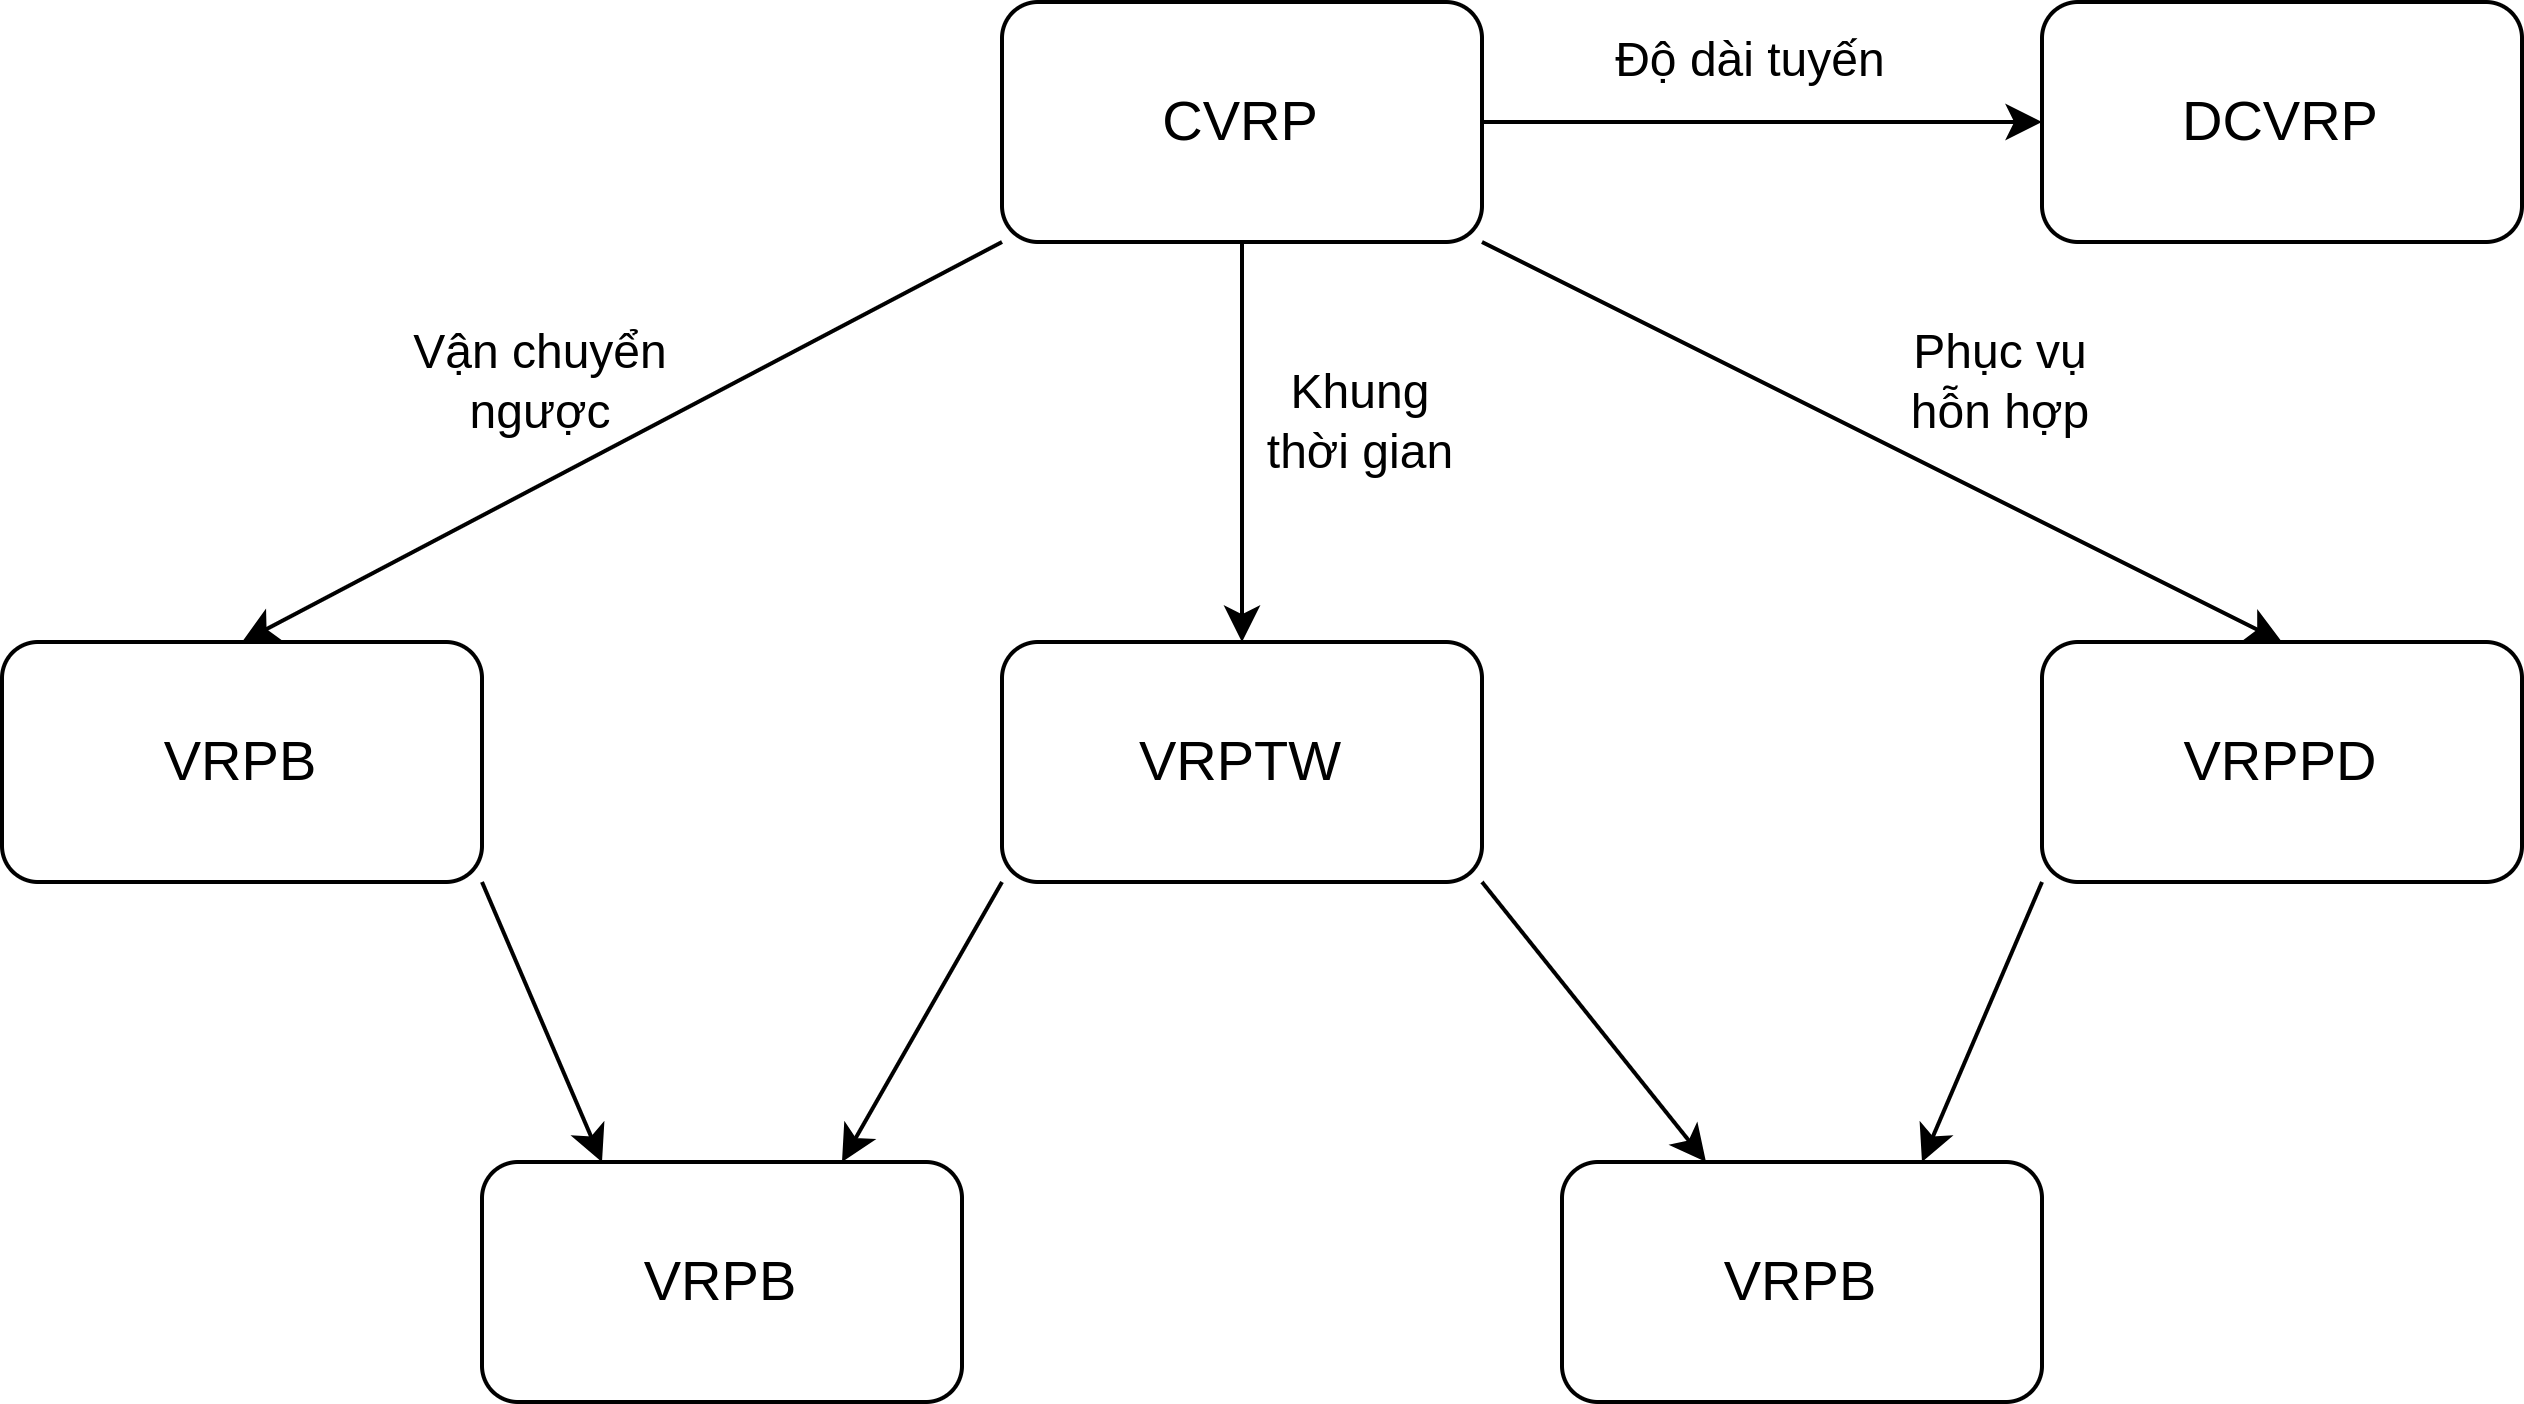
\includegraphics[width=0.8\textwidth]{figures/vrp.png} 
  \caption{Các bài toán, biến thể của VRP} % Creates caption underneath graph
  \label{fig:fg_01}
\end{figure}

\section{Định nghĩa bài toán}
\label{sec:def}

\subsection{CVRP}

Trước hết ta xem xét mô hình cho bài toán \textit{nguyên bản}: \textit{bài toán định tuyến xe với ràng buộc tải trọng}. Bài toán nguyên bản là CVRP mà không phải là VRP (không ràng buộc). Ta thấy rằng nếu không có bất kì ràng buộc nào thì một xe có thể phục vụ tất cả các yêu cầu và bài toán VRP sẽ trở thành TSP (\textit{travelling salesman problem}). Ít nhất ràng buộc về tải trọng là thực tế và giữ cho mỗi xe chỉ phục vụ được một số yêu cầu nhất định (trong trường hợp số yêu cầu không quá nhỏ cũng như tải trọng của xe là quá lớn).


Gọi $G=(V,A)$ là một độ thị đầy đủ với $V=\{ 0, ..., n \}$ là tập nút và $A$ là tập các cung. Các nút $i=1,...,n$ đại diện cho các yêu cầu hay khách hàng cần phục vụ, nút $0$ là kho hàng. Đôi khi, kho hàng cũng được biểu diễn bằng nút $n+1$.

Một số không âm được gọi là chi phí $c_{ij}$ đại diện cho mỗi cung $(i,j) \in A$. Nói cách khác, $c_{ij}$ là chi phí cần bỏ ra để di chuyển từ nút $i$ tới nút $j$. Trong bài toán này và hầu hết các bài toán định tuyến, ta không định nghĩa cạnh $(i,i)$ nên có thể gán $c_{ii} = \infty$ với $i \in V$.

Nếu đồ thị là có hướng thì ma trận chi phí $c$ là bất đối xứng, khi đó ta có bài toán CVRP bất đối xứng ACVRP (\textit{asymetric CVRP}). Ngược lại, nếu $c_{ij} = c_{ji}$ với mọi $(i,j) \in A$ ta có bài toán CVRP đối xứng SCVRP (\textit{symetric CVRP}) và các cung của $A$ được thay thế bằng tập cách cạnh vô hướng $E$. Với một cạnh $e \in E$, ta gọi $\alpha(e)$ và $\beta(e)$ là nút bắt đầu và kết thúc của cạnh.

Đồ thị $G$ phải là đồ thị liên thông và nhìn chung ta giả thiết đồ thị $G$ là đầy đủ. Với một nút $i$, gọi $\Delta^+(i)$ là tập ra của $i$ (\textit{forward star}), được định nghĩa là tập các nút $j$ mà cung $(i,j) \in A$, nói cách khác, đây là tập các nút có thể tiếp cận trực tiếp từ nút $i$. Tương tự như vậy, $\Delta^-{i}$ là tập vào của $i$ (\textit{backward star}), được định nghĩa là tập các nút $j$ mà cung $(j,i) \in A$ hay là tập các nút tiếp cận trực tiếp tới nút $i$. Với một tập nút con $S \subseteq V$, gọi $\delta(S)$ là tập các cạnh $e \in E$ chỉ có một hoặc cả hai đầu mút thuộc $S$. Để thuận tiện, khi xét một nút $i \in V$, ta viết $\delta(i)$ thay cho $\delta(\{i\})$.

Trong hầu hết các bài toán thực tế, ma trận chi phí thỏa mãn bất đẳng thức tam giác
\begin{equation}
	c_{ij} + c_{jk} \geq c_{ik}, \quad \forall i,j,k \in V.
\end{equation}
Nói cách khác, việc đi trực tiếp từ nút $i$ tới nút $j$ luôn tốn ít chi phí hơn là đi gián tiếp. Với nhiều thuật toán, bất đẳng thức tam giác là điều kiện cần, điều này có thể được đảm bảo bằng cách thêm một đại lượng dương lớn (hợp lý) vào chi phí của mỗi cung. Ta chú ý thêm rằng, nếu chi phí của mỗi cung thuộc đồ thị bằng với chi phí của đường đi ngắn nhất giữa hai đầu mút của cung thì mà trận chi phí thỏa mãn bất đẳng thức tam giác.

Trong nhiều trường hợp, tập các nút nằm trên một mặt phẳng, vị trí của chúng được cho bởi tọa độ và chi phí $c_{ij}$ của mỗi cung $(i,j) \in A$ là khoảng cách Euclide giữa hai điểm ứng với nút $i$ và $j$. Khi đó, ma trận chi phí là đối xứng và thỏa mãn bất đẳng thức tam giác. Bài toán này được gọi là \textit{Euclidian} SCVRP.

Mỗi khách hàng $i$ có một nhu cầu (về tải trọng) là $d_i$ và nhu cầu của kho $d_0=0$. Với một tập nút $S \subseteq V$, ta kí hiệu $d(S) = \sum_{i \in S} d_i$ là tổng nhu cầu của tập.

Một tập hợp $K$ đại diện cho các xe, mỗi xe có tải trọng $C$, các xe sẵn sàng ở kho tại thời điểm bắt đầu. Ta giả thiết $d_i \leq C$ với mỗi $i=1,...,n$. Điều kiện này này là cần thiết để  mỗi khách hàng đều được phục vụ. Mỗi xe phục vụ nhiều nhất một tuyến và ta giả thiết $K$ không nhỏ hơn $K_{min}$ với $K_{min}$ là số xe ít nhất cần để phục vụ toàn bộ khách hàng.

Với một tập $S \subseteq V \setminus \{0\}$, ta gọi $r(S)$ là số xe ít nhất để phục vụ toàn bộ khách hàng thuộc tập $S$. Chú ý rằng $r(V \setminus \{0\}) = K_{min}$.

CVRP yêu cầu tìm một tập chính xác $K$ các chu trình đơn (mỗi chu trình ứng với một tuyến đường) với tổng chi phí của tất cả các cung thuộc các chu trình này là nhỏ nhất. Lời giải phải thỏa mãn các ràng buộc sau
\begin{itemize}
	\item[] (i) mỗi chu trình đều đi qua nút ứng với kho hàng;
	\item[] (ii) mỗi nút ứng với một khách hàng được đi qua bởi đúng một chu trình;
	\item[] (iii) tổng nhu cầu của các khách hàng trong mỗi chu trình không được vượt quá tải trọng của xe.
\end{itemize}

\subsection{VRPTW}
Bài toán định tuyến xe với ràng buộc thời gian - VRPTW (\textit{VRP with time windows}) là một mở rộng của CVRP. Trong đó, ngoài ràng buộc về tải trọng cho mỗi xe, mỗi khách hàng $i$ bị ràng buộc bởi một khoảng thời gian $[a_i, b_i]$ được gọi là khung thời gian hay cửa sổ thời gian (\textit{time window}). Thời gian phục vụ khách hàng $i$ là $s_i$. Thời gian di chuyển từ nút $i$ tới nút $j$ là $t_{ij}$ với mỗi cung $(i,j) \in A$ hay $t_e$ với $e \in E$. Ngoài ra nếu xe đến nút $i$ sớm thì phải chờ đến thời gian $a_i$ mới được phục vụ. Nếu xe đến nút $i$ muộn hơn $b_i$ thì khách hàng sẽ không được phục vụ.

Thường thì ma trận chi phí và ma trận thời gian di chuyển là như nhau, hơn nữa các xe được giả thiết đều xuất phát từ kho tại thời điểm $0$. Ràng buộc thời gian dẫn tới việc mỗi tuyến đường là có hướng (có thứ tự đi đến các nút) ngay cả khi ma trận chi phí là đối xứng. Chính vì thế, VRPTW thường được mô tả như một bài toán bất đối xứng.

VRPTW yêu cầu tìm một tập chính xác $K$ chu trình đơn với tổng chi phí là nhỏ nhất, thỏa mãn các ràng buộc sau đây
\begin{itemize}
	\item[] (i) mỗi chu trình đều đi qua nút ứng với kho hàng;
	\item[] (ii) mỗi nút ứng với một khách hàng được đi qua bởi đúng một chu trình;
	\item[] (iii) tổng nhu cầu của các khách hàng trong mỗi chu trình không được vượt quá tải trọng của xe;
	\item[] (iv) với mỗi khách hàng $i$, thời gian bắt đầu phục vụ phải nằm trong khung thời gian $[a_i, b_i]$ và xe hoàn thành việc phục vụ sau khoảng thời gian $s_i$.
\end{itemize}

VRPTW là bài toán NP-khó, nó là trường hợp tổng quát của CVRP. Nếu ta đặt $a_i=0$ và $b_i=\infty$ với $i \in V \setminus \{0\}$ thì VRPTW trở thành CVRP. Ngoài ra ta cũng thu được biến thể TSP với ràng buộc thời gian (TSPTW) nếu $C \geq d(V)$ và $K=1$.

\subsection{VRPPD}
Một biến thể khác nữa của CVRP là bài toán định tuyến xe với lấy và giao hàng (\textit{VRP with pickup and delivery - VRPPD}). Trong đó, mỗi khách hàng $i$ có thêm hai đại lượng đặc trưng nữa là $d_i$ và $p_i$ lần lượt là nhu cầu lấy và giao (của khách hàng) tại vị trí của khách hàng $i$. Đôi khi, ta chỉ dùng một đại lượng $d_i = d_i - p_i$ cho mỗi khách hàng $i$ để chỉ lượng nhu cầu chênh lệch giữa việc lấy và giao hàng (có thể là số âm). Với mỗi khách hàng $i$, gọi $O_i$ là nút đại diện cho điểm giao hàng và $D_i$ là nút đại diện cho điểm lấy hàng.

Với mỗi khách hàng, ta giả thiết điểm giao được phục vụ trước điểm lấy. Do đó, tải hiện tại của một xe trướ khi tới điểm đã cho là tải ban đầu trừ đi tổng nhu cầu đã giao cộng với tổng nhu cầu đã lấy.

VRPPD yêu cầu tìm chính xác một tập $K$ các chu trình đơn với tổng chi phí là nhỏ nhất, thỏa mãn các ràng buộc sau đây

\begin{itemize}
	\item[] (i) mỗi chu trình đều đi qua nút ứng với kho hàng;
	\item[] (ii) mỗi nút ứng với một khách hàng được đi qua bởi đúng một chu trình;
	\item[] (iii) tải hiện tại của xe trong suốt quá trình phục vụ không âm và không được vượt quá tải trọng của xe;
	\item[] (iv) với mỗi khách hàng $i$, khách hàng $O_i$ khác với kho phải được phục vụ trong cùng một tuyến và trước khách hàng $i$;
	\item[] (v) với mỗi khách hàng $i$, khách hàng $D_i$ khác với kho phải được phụ vụ trong cùng một tuyến và sau khách hàng $i$.
\end{itemize}

VRPPD là trường hợp tổng quát của CVRP. Nếu ta đặt $O_i = D_i = 0$ và $p_i = 0$ cho mọi $i \in V$ thì VRPPD suy biến về CVRP. Hơn nữa nếu đặt $K=1$ thì ta thu được TSP với lấy và giao hàng (\textit{TSP with pickup and delivery - TSPPD}).

\section{Mô hình toán học}
\label{sec:math}

Phần tiếp theo, ta trình bày một số mô hình toán học cơ bản cho VRP theo P. Toth và D. Vigo \cite{toth2002vehicle}. Mô hình cụ thể cho VRPTW được trình bày ở phần \ref{sec:math_vrptw}. 

\subsection{Các mô hình cơ bản cho VRP}
\label{sec:math_common}

Trong phần này, chúng ta cùng xem xét các mô hình toán học cơ bản cho VRP và xem xét cách các mô hình này được mở rộng để kết hợp hay bổ sung ràng buộc hoặc hàm mục tiêu.

Có ba cách tiếp cận để mô hình hóa VRP. Loại mô hình đầu tiên là "công thức dòng xe" (\textit{vehicle flow formulations}) sử dụng các biến nguyên ứng với mỗi cung hay cạnh của đồ thị. Các biến này để đếm số lần mà xe đi qua cung hay cạnh đó. Loại mô hình này thường được sử dụng cho những phiên bản cơ bản của VRP. Mô hình đặc biệt phù hợp cho những trường hợp mà tổng chi phí, hay hàm mục tiêu có thể biểu diễn bằng tổng chi phí của mỗi cung hay cạnh và hầu hết các ràng buộc liên quan đến sự thay đổi giữa các yêu cầu trong cùng một tuyến. Khi đó, mô hình có thể được xây dựng một cách hiệu quả qua việc định nghĩa hợp lý tập cung và chi phí của cung. Tuy nhiên, "công thức dòng xe" không được sử dụng cho các bài toán mà tổng chi phí phụ thuộc vào chuỗi (có thứ tự) các nút hoặc phụ thuộc vào loại phương tiện.

Loại mô hình thứ hai là "công thức dòng hàng" (\textit{commodity flow formulation}). Trong loại mô hình này, các biến nguyên ứng với mỗi cung hoặc cạnh biểu diễn "dòng" của lượng hàng dọc theo các tuyến đường. "Công thức dòng hàng" thường được sử dụng làm cơ sở cho các phương pháp giải chính xác VRP.

Loại mô hình cuối cùng có số biến nhị phân tăng theo cấp số nhân với kích thước của đầu vào, mỗi biến biểu thị cho một chu trình khả thi khác nhau. Trong loại mô hình này, VRP được mô hình hóa như một bài toán phân hoạch tập hợp (\textit{Set-Partitioning Problem - SPP}). SSP xác định một tập các chu trình có chi phí nhỏ nhất phục vụ mỗi yêu càu một lần và thỏa mãn các ràng buộc. Ưu điểm chính của loại mô hình này là nó cho phép tổng quát hóa chi phí của các tuyến đường ví dụ như khi chi phí của tuyến phụ thuộc vào toàn bộ chuỗi các cung hay cạnh và phụ thuộc vào loại xe. Hơn nữa, các ràng buộc không cần tính đến tính khả thi của một tuyến đường đơn lẻ. Kết quả là ràng buộc có thể được thay thế bằng các bất đẳng thức gọn gàng hơn. Đánh đổi lại, loại mô hình này cần một số lượng biến biểu diễn rất lớn.

\subsubsection*{Mô hình dòng xe}

Trước tiên, chúng ta mô tả công thức "lập trình tuyến tính nguyên" (\textit{integer linear programming}) cho ACVRP, sau đó là SCVRP. Mô hình "công thức dòng xe hai chỉ số" (\textit{two-index vehicle flow formulation}) sử dụng $O(n^2)$ biến nhị phân $x$ để chỉ thị nếu một xe đi qua cung $(i,j)$ hay không. Nói cách khác, $x_{ij}$ nhận giá trị bằng $1$ nếu cung $(i, j) \in A$ nằm trong nghiệm tối ưu và $0$ nếu trong trường hợp còn lại. 

\begin{equation} \label{eq:vrp1}
  \text{(VRP1)} \quad \min \sum_{i \in V} \sum_{j \in V} c_{ij} x_{ij}
\end{equation}
s.t.
\begin{flalign}
	\label{ct_vrp1:1}  & \sum_{i \in V} x_{ij} = 1, \quad \forall j \in V \setminus \{0\}, \\
  \label{ct_vrp1:2}  & \sum_{j \in V} x_{ij} = 1, \quad \forall i \in V \setminus \{0\}, \\
  \label{ct_vrp1:3}  & \sum_{i \in V} x_{i0} = K, \\
  \label{ct_vrp1:4}  & \sum_{j \in V} x_{0j} = K, \\
  \label{ct_vrp1:5}  & \sum_{i \notin  S} \sum_{j \in S} x_{ij} \geq r(S), \quad \forall S \subseteq V \setminus \{0\}, S \neq \emptyset, \\
  \label{ct_vrp1:6}  & x_{ij} \in \{0,1\}, \quad \forall i,j \in V.
\end{flalign}
Ràng buộc (\ref{ct_vrp1:1}) và (\ref{ct_vrp1:2}) đảm bảo chỉ có đúng một cung vào và một cung ra cho mỗi nút ứng với mỗi yêu cầu. Ràng buộc (\ref{ct_vrp1:3}) và (\ref{ct_vrp1:4}) đảm bảo có đúng $K$ xe xuất phát từ kho và trở về kho. Ràng buộc (\ref{ct_vrp1:5}) đảm bảo số xe được sử dụng không nhỏ hơn số xe tối thiểu cần để phục vụ tất cả các yêu cầu. Trong thực tế, nhiều khi ràng buộc này được phát biểu lại là tổng số xe sử dụng không vượt quá một giới hạn trên $K_{max}$ nhất định. 

Đối với hệ đối xứng, \textit{VRP1} được viết lại như sau

\begin{equation} \label{eq:vrp2}
	\text{(VRP2)} \quad \min \sum_{i \in V \setminus \{n\}} \sum_{j > i} c_{ij} x_{ij}
\end{equation}
s.t.
\begin{flalign}
	\label{ct_vrp2:1}  & \sum_{h < i} x_{hi} + \sum_{j < i} x_{ij} = 2, \quad \forall j \in V \setminus \{0\}, \\
  \label{ct_vrp2:2}  & \sum_{j \in V \setminus \{0\}} x_{0j} = 2K, \\
  \label{ct_vrp2:3}  & \sum_{i \in S} \sum_{h < i, h \notin S} x_{hi} + \sum_{i \in S} \sum_{j < i, j \notin S} x_{ij} \geq 2r(S), \quad \forall S \subseteq V \setminus \{0\}, S \neq \emptyset, \\
  \label{ct_vrp2:4}  & x_{ij} \in \{0,1\}, \quad \forall i,j \in V \setminus \{0\}, i < j, \\
  \label{ct_vrp2:5}  & x_{0j} = \{0, 1, 2\}, \quad \forall i \in V \setminus \{0\}.
\end{flalign}
Ràng buộc (\ref{ct_vrp2:1}) và (\ref{ct_vrp2:2}) đảm bảo chỉ có đúng một cung vào và một cung ra cho mỗi nút ứng với mỗi yêu cầu, $2K$ để đảm bảo số xe xuất phát và kết thúc tại kho. Ràng buộc (\ref{ct_vrp2:3}) đảm bảo số xe được sử dụng không nhỏ hơn số xe tối thiểu cần để phục vụ tất cả các yêu cầu. 

Phiên bản mô hình 2 chỉ số cho trường hợp hệ đối xứng có thể được biểu diễn chỉ với một chỉ số $e$ biểu thị cho cạnh vô hướng $e \in E$. Nếu ta không cho phép tuyến chỉ chứa đúng một yêu cầu thì các biến sử dụng đều là nhị phân. Ngoài ra, nếu $e \notin \delta(0)$ thì $x_e \in \{0, 1\}$ và nếu $e \in \delta(0)$ thì $x_e \in \{0, 1, 2\}$. Công thức \textit{VRP2} được viết lại như sau

\begin{equation} \label{eq:vrp3}
	\text{(VRP3)} \quad \min \sum_{e \in E} c_e x_e
\end{equation}
s.t.
\begin{flalign}
	\label{ct_vrp3:1}  & \sum_{e \in \delta(i)} x_e = 2, \quad \forall i \in V \setminus \{0\}, \\
  \label{ct_vrp3:2}  & \sum_{e \in \delta(0)} x_e = 2K, \\
  \label{ct_vrp3:3}  & \sum_{e \in \delta(S)} x_e \geq 2r(S), \quad \forall S \subseteq V \setminus \{0\}, S \neq \emptyset, \\
  \label{ct_vrp3:4}  & x_e \in \{0,1\}, \quad \forall e \notin \delta(0), \\
  \label{ct_vrp3:5}  & x_e \in \{0,1,2\}, \quad \forall e \in \delta(0).
\end{flalign}

Mô hình dòng xe hai chỉ số được sử dụng khá rộng rãi trong các biến thể cơ bản của SCVRP và ACVRP chẳng hạn như VRPB. Tuy nhiên, mô hình này là không đủ mạnh cho các biến thể phức tạp hơn ví dụ như khi tổng chi phí phụ thuộc vào một chuỗi (có thứ tự) các nút hoặc phụ thuộc vào loại phương tiện. Ngoài ra, ta cũng không biết một cách tường minh xe nào được dùng cho tuyến đường. 

Một mô hình mở rộng để khắc phục các điểm yếu của mô hình dòng xe hai chỉ số là mô hình dòng xe ba chỉ số (\textit{three-index vehicle flow formulation}). Mô hình này sử dụng $O(n^2K)$ biến nhị phân $x$. Biến $x_{ijk}$ đếm số lần cung $(i, j) \in A$ được đi qua bởi xe $k$ với $k=1,...,K$ trong nghiệm tối ưu. Ngoài ra ta sử dụng thêm $O(nK)$ biến nhị phân $y$, với $y_{ik}$ ($i \in V; k=1,...,K$) nhận giá trị $1$ nếu yêu cầu $i$ được phục vụ bởi xe $k$ và $0$ trong trường hợp còn lại. Mô hình ba chỉ số cho ACVRP được mô tả như sau

\begin{equation} \label{eq:vrp4}
	\text{(VRP4)} \quad \min \sum_{i \in V} \sum_{j \in V} c_{ij} \sum_{k=1}^K x_{ijk}
\end{equation}
s.t.
\begin{flalign}
	\label{ct_vrp4:1}  & \sum_{k=1}^K y_{ik} = 1, \quad \forall i \in V \setminus \{0\}, \\
  \label{ct_vrp4:2}  & \sum_{k=1}^K y_{0k} = K, \\
  \label{ct_vrp4:3}  & \sum_{j \in V} x_{ijk} = \sum_{j \in V} x_{jik} = y_{ik}, \quad \forall i \in V \setminus \{0\}, k=1,...,K, \\
  \label{ct_vrp4:4}  & \sum_{i \in V} d_i y_{ik} \leq C, \quad \forall k=1,...,K, \\
  \label{ct_vrp4:5}  & \sum_{i \in S} \sum_{j \notin S} x_{ijk} \geq y_{hk}, \quad \forall S \subseteq V \setminus \{0\}, h \in S, k=1,...,K, \\
  \label{ct_vrp4:6}  & y_{ik} \in \{0,1\}, \quad \forall i \in V, k=1,...,K, \\
  \label{ct_vrp4:7}  & x_{ijk} \in \{0,1\}, \quad \forall i,j \in V, k=1,...,K.
\end{flalign}
Ràng buộc (\ref{ct_vrp4:1}) đảm bảo mỗi yêu cầu được phục vụ đúng một lần. Ràng buộc (\ref{ct_vrp4:2}) đảm bảo có $K$ xe xuất phát từ kho. Ràng buộc (\ref{ct_vrp4:3}) đảm bảo có cùng số xe đến và rời khỏi vị trí của mỗi yêu cầu. Ràng buộc (\ref{ct_vrp4:4}) là ràng buộc về tải trọng của xe. Ràng buộc (\ref{ct_vrp4:5}) đảm bảo tính kết nối trong tuyến đường được phục vụ bởi xe $k$.

Đối với bài toán đối xứng, ta có phiên bản hai chỉ số cho mô hình trên với biến nhị phân $x_{ek}$, $e \in E$ và $k=1,...,K$

\begin{equation} \label{eq:vrp5}
	\text{(VRP5)} \quad \min \sum_{e \in E} c_{ij} \sum_{k=1}^K x_{ek}
\end{equation}
s.t.
\begin{flalign}
	\label{ct_vrp5:1}  & \sum_{k=1}^K y_{ik} = 1, \quad \forall i \in V \setminus \{0\}, \\
  \label{ct_vrp5:2}  & \sum_{k=1}^K y_{0k} = K, \\
  \label{ct_vrp5:3}  & \sum_{e \in \delta(i)} x_{ek} = 2y_{ik}, \quad \forall i \in V, k=1,...,K, \\
  \label{ct_vrp5:4}  & \sum_{i \in V} d_i y_{ik} \leq C, \quad \forall k=1,...,K, \\
  \label{ct_vrp5:5}  & \sum_{e \in \delta(S)} x_{ijk} \geq 2y_{hk}, \quad \forall S \subseteq V \setminus \{0\}, h \in S, k=1,...,K, \\
  \label{ct_vrp5:6}  & y_{ik} \in \{0,1\}, \quad \forall i \in V, k=1,...,K, \\
  \label{ct_vrp5:7}  & x_{ek} \in \{0,1\}, \quad \forall e \notin \delta(0), k=1,...,K, \\
  \label{ct_vrp5:8}  & x_{ek} \in \{0,1,2\}, \quad \forall e \in \delta(0), k=1,...,K.
\end{flalign}

Công thức dòng xe ba chỉ số được sử dụng cho các biến thể  VRP với nhiều ràng buộc ví dụ như VRPTW. Công thức này được trình bày trong phần \ref{sec:math_vrptw}. Công thức dòng hàng và công thức phân hoạch tập hợp được trình bày trong chương \ref{chap:solution}.

\subsection{Mô hình cho biến thể VRPTW}
\label{sec:math_vrptw}

Trong phần này, ta trình bày biểu diễn toán học cho bài toán VRPTW. Trong khuôn khổ luận văn này, tác giả tập trung thực nghiệm giải quyết VRPTW, từ đó ta cũng có thể giản ước về CVRP cũng như tổng quát với VRPPD (\textit{VRP with pickup and delevery}) hoặc PDPTW (\textit{pickup and delivery with time window}). Như đã trình bày ở phần trước, VRPTW là một mở rộng của CVRP với ràng buộc khung thời gian. Trong đó, mỗi khách hàng $i$ được ràng buộc bởi một khung thời gian $[a_i,b_i]$. Xe không được đến $i$ tại thời điểm $t_i > b_i$, ngoài ra, nếu đến sớm hơn thởi điểm $a_i$ hay $t_i < a_i$ thì xe cần phải chờ tới thời điểm $a_i$ để phục vụ khách hàng. Thời gian phục vụ của khách hàng $i$ là $s_i$.

VRPTW là bài toán NP-khó, việc tìm lời giải hay nghiệm tối ưu (chính xác) gần như là bất khả thi với các bài toán có kích thước đầu vào lớn. Để dễ hình dung, xét bài toán VRP, với số lượng khách hàng $n=100$, và chỉ một xe, số lượng lời giải là $n! \approx 10^{158}$. Nếu ta có số CPU ước tính bằng toàn bộ số nguyên tử trong vũ trụ $n_{CPU} \approx 10^{80}$, thời gian nhỏ nhất là thời gian Plank $t_p \approx 5.39 \times 10^{-44}$. Để kiểm tra toàn bộ lời giải có phải nghiệm tối ưu ta cần thời gian $T \approx 10^{158} \times 5.39 \times 10^{-44} / 10^{80} \approx 5.39 \times 10^{34}$. Để so sánh, tuổi của vũ trụ được ước tính khoảng $4.33 \times 10^{17}$. Nghĩa là ta sẽ mất thời gian lớn gấp cỡ \textit{một trăm triệu tỉ} lần tuổi của cả vũ trụ! \footnote[1]{Slides của Thibaut Vidal (SOICT, Nha Trang 2017)}

Như đã trình bày ở phần \ref{sec:def}, VRPTW được định nghĩa trên đồ thị $G = (V, A)$, kho hàng được biểu diễn bởi nút $0$ và $n+1$. Một tuyến thỏa mãn là một đường đi trên đồ thị $G$ bắt đầu từ $0$ và kết thúc ở $n+1$. Nếu kho hàng được biểu diễn chỉ bởi nút $0$ thì tuyến thỏa mãn là một đơn chu trình trên đồ thị $G$ chứa nút $0$. Khung thời gian của nút $0$ và $n+1$ là $[a_0, b_0] = [a_{n+1}, b_{n+1}] = [E, L]$, trong đó $E$ và $L$ lần lượt là thời gian sớm nhất rời kho và thời gian muộn nhất trở về kho. Ngoài ra, thời gian phục vụ và nhu cầu của kho đều được đặt bằng 0, hay $s_0 = s_{n+1} = 0$ và $d_0 = d_{n+1} = 0$. Lời giải chấp nhận được chỉ tồn tại nếu $a_0 = E \leq \min_{i \in V \setminus \{0\}} \{b_i - t_{0i}\}$ và $b_{n+1} = L \geq \min_{i \in V \setminus \{0\}} \{ a_i + s_i + t_{0i} \}$. Chú ý rằng, cung $(i,j) \in A$ có thể được bỏ đi nếu không thỏa mãn ràng buộc thời gian $a_i + s_i + t_{ij} > b_j$ hoặc vi phạm ràng buộc về tải trọng $d_i + d_j > C$. Cuối cùng, nếu mục tiêu chính là giảm thiểu số lượng xe thì cung $(0,n+1)$ với $c_{0,n+1} = t_{0,n+1} = 0$ phải được thêm vào $A$.

Tiếp theo, chúng ta trình bày một mô hình toán cho VRPTW với hai biến: biến $x_{ijk}$ (\textit{flow variable}) với $(i,j) \in A, k \in K$ nhận giá trị 1 nếu xe $k$ đi trực tiếp từ nút $i$ tới nút $j$ và 0 nếu ngược lại. Biến $w_{ik}$ với $i \in V, k \in K$ là thời gian bắt đầu phục vụ khách hàng $i$ bởi xe $k$. VRPTW được mô hình một cách chính tắc như sau theo Toth (2002) \cite{toth2002vehicle}

\begin{equation} \label{eq1}
	\min \sum_{k \in K} \sum_{(i,j) \in A} c_{ij} x_{ijk}
\end{equation}
s.t.
\begin{flalign}
	\label{ct:1}  & \sum_{k \in K} \sum_{j \in \Delta^+(i)} x_{ijk} = 1, \quad \forall i \in N, \\
	\label{ct:2}  & \sum_{j \in \Delta^+(0)} x_{0jk} = 1, \quad \forall k \in K,                   \\
	\label{ct:3}  & \sum_{i \in \Delta^-(j)} x_{ijk} -  \sum_{i \in \Delta^+(j)} x_{jik} = 0, \quad \forall k \in K, j \in N, \\
	\label{ct:4}  & \sum_{i \in \Delta^-(n+1)} x_{i,n+1,k} = 1, \quad \forall k \in K, \\
	\label{ct:5}  & x_{ijk} (w_{ik} + s_i + t_{ij} - w_{jk}) \leq 0, \quad \forall k \in K, (i,j) \in A, \\
	\label{ct:6}  & a_i \sum_{j \in \Delta^+(i)} x_{ijk} \leq w_{ik} \leq b_i \sum_{j \in \Delta^+(i)} x_{ijk}, \quad \forall k \in K, i \in N, \\
	\label{ct:7}  & E \leq w_{ik} \leq L, \quad \forall k \in K, i \in \{0, n+1\}, \\
	\label{ct:8}  & \sum_{i \in N} d_i \sum_{j \in \Delta^+(i)} x_{ijk} \leq C, \quad \forall k \in K, \\
	\label{ct:9}  & x_{ijk} \geq 0, \quad \forall k \in K, (i,j) \in A, \\
	\label{ct:10} & x_{ijk} \in \{0,1\}, \quad \forall k \in K, (i,j) \in A.
\end{flalign}
Hàm mục tiêu trong phương trình (\ref{eq1}) biểu diễn tổng chi phí của tất cả các tuyến đường.
Tập $N = V \setminus \{0\}$ biểu diễn cho tập khách hàng.

\begin{itemize}
	\item Ràng buộc (\ref{ct:1}) đảm bảo rằng mỗi khách hàng chỉ được phục vụ bởi một xe.
	\item Ràng buộc (\ref{ct:2}) đảm bảo rằng mỗi xe phải xuất phát từ kho hàng.
	\item Ràng buộc (\ref{ct:3}) đảm bảo rằng trên một tuyến, nếu khách hàng $i$ được phục vụ thì trước và sau đó đều có một khách hàng khác được phục vụ hoặc trước và sau đó là kho hàng. Nói cách khác, khách hàng $i$ phải ở giữa tuyến.
	\item Ràng buộc (\ref{ct:4}) đảm bảo rằng mỗi xe phải trở về kho hàng.
	\item Ràng buộc (\ref{ct:5}) đảm bảo về khung thời gian khi xe đi từ khách hàng $i$ tới khách hàng $j$. Nếu xe $k$ đi từ khách hàng $i$ tới khách hàng $j$ thì thời gian bắt đầu phục vụ khách hàng $i$ cộng với thời gian phục vụ khách hàng $i$ cộng với thời gian di chuyển từ khách hàng $i$ tới khách hàng $j$ phải nhỏ hơn hoặc bằng thời gian bắt đầu phục vụ khách hàng $j$. Dấu bằng xảy ra khi xe đến $j$ sau thời điểm $a_j$ (khách hàng $j$ được phục vụ luôn), nếu đến sớm hơn thì xe phải chờ để phục vụ khách hàng.
	\item Ràng buộc (\ref{ct:6}) đảm bảo rằng thời gian bắt đầu phục vụ khách hàng $i$ bởi xe $k$ nằm trong khung thời gian $[a_i, b_i]$.
	\item Ràng buộc (\ref{ct:7}) đảm bảo rằng thời gian bắt đầu phục vụ khách hàng $i$ bất kì phải nằm trong khoảng thời gian từ sớm nhất xuất phát từ kho và muộn nhất về kho.
	\item Ràng buộc (\ref{ct:8}) đảm bảo rằng tổng tải của mỗi xe không được vượt quá tải trọng tối đa $C$.
	\item Ràng buộc (\ref{ct:9}) và (\ref{ct:10}) đảm bảo điều kiện nhị phân của \textit{flow variable} $x_{ijk}$.
\end{itemize}

Ta có thể nhận thấy rằng, ràng buộc (\ref{ct:6}) ép $w_{ik} = 0$ nếu như khách hàng $i$ không được phục vụ bởi xe $k$. Điều kiện nhị phân trong ràng buộc (\ref{ct:10}) cho phép ràng buộc (\ref{ct:5}) được thay thế bởi
\begin{equation}
	\label{ct:5'}
	w_{ik} + s_i + t_{ij} - w_{jk} \leq (1 - x_{ijk}) M_{ij}, \quad \forall k \in K, (i,j) \in A,
\end{equation}
với $M_{ij}$ là các hằng số rất lớn. Hơn nữa $M_{ij}$ có thể thay bằng $\max \{b_i + s_i + t_{ij} - a_j, 0\}$ với $(i,j) \in A$ và như vậy ta chỉ cần kiểm tra ràng buộc (\ref{ct:5}) và (\ref{ct:5'}) cho các cung $(i, j) \in A$ thỏa mãn $M_{ij} > 0$. Mặt khác, khi $\max \{b_i + s_i + t_{ij} - a_j, 0\} = 0$ các điều kiện này được thỏa mãn với mọi $w_{ik}$, $w_{jk}$ và $x_{ijk}$.

Chúng ta không cần đưa ra mô hình cho CVRP nữa, bởi ta có thể bỏ qua các ràng buộc về thời gian ở điều kiện từ (\ref{ct:5}) đến (\ref{ct:7}). Khi đó VRPTW sẽ trở thành CVRP như đã trình bày ở những phần trước đó. Tác giả cũng không đưa ra mô hình cho VRPPD hay PDPTW để tránh sự phức tạp. VRPTW vừa đủ để ta có một mô hình đẹp và thực tế.
        \chapter{Một số phương pháp cho VRP}
\label{chap:solution}

Trong chương này, chúng ta sẽ xem xét một số khái niệm cần thiết và phương pháp để giải (lớp) bài toán định tuyến xe. Trong suốt chặng đường hơn 60 năm của bài toán VRP, có rất nhiều phương pháp được nghiên cứu và thực nghiệm từ các thuật toán giải chính xác đến các thuật toán xấp xỉ. Ba lớp thuật toán được trình bày bao gồm \textit{thuật toán chính xác}, \textit{heuristics cổ điển} và \textit{metaheuristics}. Lớp các thuật toán được trình bày một cách khái quát theo G. Laporte \cite{laporte2009fifty}. Cuối cùng tác giả đưa ra lựa chọn và đi sâu vào thuật toán tìm kiếm lân cận rộng thích ứng - ALNS (\textit{Adaptive Large Neighborhood Search}) để giải quyết bài toán VRPTW trong luận văn này.

\section{Thuật toán chính xác}

\subsection{Nhánh và cận}

Một trong những thuật toán chính xác được nghiên cứu sớm nhất là \textit{nhánh và cận}, lần đầu xuất hiện trong bài báo \textit{"An Algorithm for the Vehicle Dispatching Problem"} của N. Christofides và S. Eilon năm 1969 \cite{christofides1969algorithm}. Với $m$ là tham số đầu vào, đầu tiên đồ thị được mở rộng với việc thêm vào $m-1$ kho ảo và đặt chi phí của chúng bằng một số vô cùng lớn. Sau đó giải bài toán m-TSP trên đồ thị này bằng thuật toán TSP được trình bày bởi Little et al. (1963) \cite{little1963algorithm}

Hiệu năng của các thuật toán nhánh-cận đầu tiên được cải thiện đáng kể hai phương pháp cận dưới là k-degree centre trees (k-DCT) và q-routes (Christofides et al. (1981) \cite{christofides1981exact}).

\subsection{Quy hoạch động}

Eilon, Watson-Gandy và Christofides (1971) \cite{christofides1969algorithm} đưa ra lời giải cho bài toán VRP bằng phương pháp quy hoạch động. Gọi $c(S)$ là chi phí tối ưu của một tuyến ứng với tập nút $S \subseteq V \setminus \{0\}$. Mục tiêu là cực tiểu hóa $\sum_{r=1}^{m} c(S_r)$ trên tất cả các quy hoạch khả dĩ $\{S_1,...,S_m\}$ của $V \setminus \{0\}$. Gọi $f_k(U)$ là chi phí nhỏ nhất có thể đạt được khi sử dụng $k$ xe cho một tập con $U$ của $V \setminus \{0\}$. Ta có
\begin{equation}
	\label{eq:dp}
	f_k(U) =
	\begin{cases}
		c(U) \quad \text{nếu } k = 1,                                                                                      \\
		\min_{U^* \subseteq U \subseteq V \setminus \{0\}} \{f_{k-1} (U \setminus U^*) + c(U^*)\} \quad \text{nếu } k > 1. \\
	\end{cases}
\end{equation}
Chi phí tối ưu là $f_m(V \setminus \{0\})$ và các tuyến là các phân hoạch của $V \setminus \{0\}$ theo phương trình (\ref{eq:dp}).

\subsection{Công thức dòng xe}
Công thức 2-chỉ số cho bài toán VRP được nghiên cứu đầu tiên bởi Laporte, Nobert (1983) \cite{laporte1983branch} và Laporte, Nobert, Desrochers (1985) \cite{laporte1985optimal} và mở rộng công thức TSP cổ điển của Dantzig, Fulkerson, Johnson (1954) \cite{dantzig1954solution}. Gọi $x_{ij}$ là biến 0-1-2 bằng số lần một xe đi qua cung $(i,j)$. Bài toán được mô hình hóa như sau
\begin{equation}
	\min \sum_{(i,j) \in E} c_{ij} x_{ij}
\end{equation}
s.t.
\begin{flalign}
	\label{ct2:1} & \sum_{j=1}^n x_{0j}=2m, & \quad \\
	\label{ct2:2} & \sum_{i<k} x_{ik} + \sum_{j>k} x_{kj} = 2 & \quad \forall k \in V \setminus \{0\}, \\
	\label{ct2:3} & \sum_{i,j \in S} x_{ij} \leq |S| - \nu(S) & \quad \forall S \subseteq V \setminus \{0\}, \\
	\label{ct3:3} & x_{0j} \in \{0,1,2\} & \quad \forall j \in V \setminus \{0\}, \\
	\label{ct2:4} & x_{ij} \in \{0,1\} & \quad \forall i,j \in V \setminus \{0\},
\end{flalign}
trong đó $\nu(S)$ là cận dưới của số lượng xe cần thiết để phục vụ tập $S$. Công thức dòng xe và các biến thể đã được trình bày kĩ từ chương \ref{chap:model}.

\subsection{Công thức dòng hàng}
Trong công thức dòng hàng, biến $y_{ij}$ (hoặc $y_{ijk}$) định nghĩa tải (lượng hàng) của xe mang theo trên cung $(i,j)$. Ví dụ được trình bày bởi Gavish, Graves (1979) \cite{gavish1978travelling}, tuy nhiên các tác giả không đưa ra kết quả tính toán. Các ví dụ gần đây hơn được nghiên cứu bởi Baldacci, Hadjiconstantinou, Mingozzi (2004) \cite{baldacci2004exact} dựa trên mô hình TSP của Finke, Claus, Gunn
(1984) \cite{finke1984two}. Công thức cho một đồ thị mở rộng $\bar{G} = (\bar{V}, \bar{E})$, với $\bar{V} = V \cup \{ (i, n+1): i \in V \}$. Một tuyến được định nghĩa là một đường đi có hướng từ $0$ đến $n+1$. Biến nhị phân $x_{ij}$ bằng $1$ khi và chỉ khi cạnh $(i,j)$ được chọn vào tuyến. Biến $y_{ij}$ định nghĩa tải của xe trên cung $(i,j)$ và $y_{ji} = Q - y_{ij}$ biểu diễn xe rỗng trên cung $(j,i)$ mỗi khi $x_{ij} = 1$. Công thức dòng hàng được mô hình hóa như sau

\begin{equation}
	\min \sum_{(i,j) \in E} c_{ij} x_{ij}
\end{equation}
s.t.
\begin{flalign}
	\label{ct3:1} & \sum_{j \in \bar{V}} (y_{ji} - y_{ij}) = 2q_i & \quad \forall i \in V \setminus \{0\}, \\
	\label{ct3:2} & \sum_{j \in V \setminus \{0\}} y_{0j} = \sum_{i \in V \setminus \{0\}} q_i, & \quad \\
	\label{ct3:3} & \sum_{j \in V \setminus \{0\}} y_{j0} = mQ - \sum_{i \in V \setminus \{0\}} q_i, & \quad \\
	\label{ct3:4} & \sum_{j \in V \setminus \{0\}} y_{n+1,j} = mQ, & \quad \\
	\label{ct3:5} & y_{ij} + y_{ji} = Qx_{ij} & \quad \forall (i,j) \in \bar{E}, \\
	\label{ct3:5} & \sum_{i<k} x_{ik} + \sum_{j>k} x_{kj} = 2 & \quad \forall k \in V \setminus \{0\}, \\
	\label{ct3:6} & y_{ij} \geq 0, y_{ji} \geq 0 & \quad \forall (i,j) \in \bar{E}, \\
	\label{ct3:7} & x_{ij} \in \{0,1\} & \quad \forall (i,j) \in \bar{E}.
\end{flalign}

Bài toán này được giải bằng \textit{branch-and-cut} với các bất đẳng thức VRP được biểu diễn theo các biến $x_{ij}$

\begin{figure}[H] % places figure environment here   
  \centering % Centers Graphic
  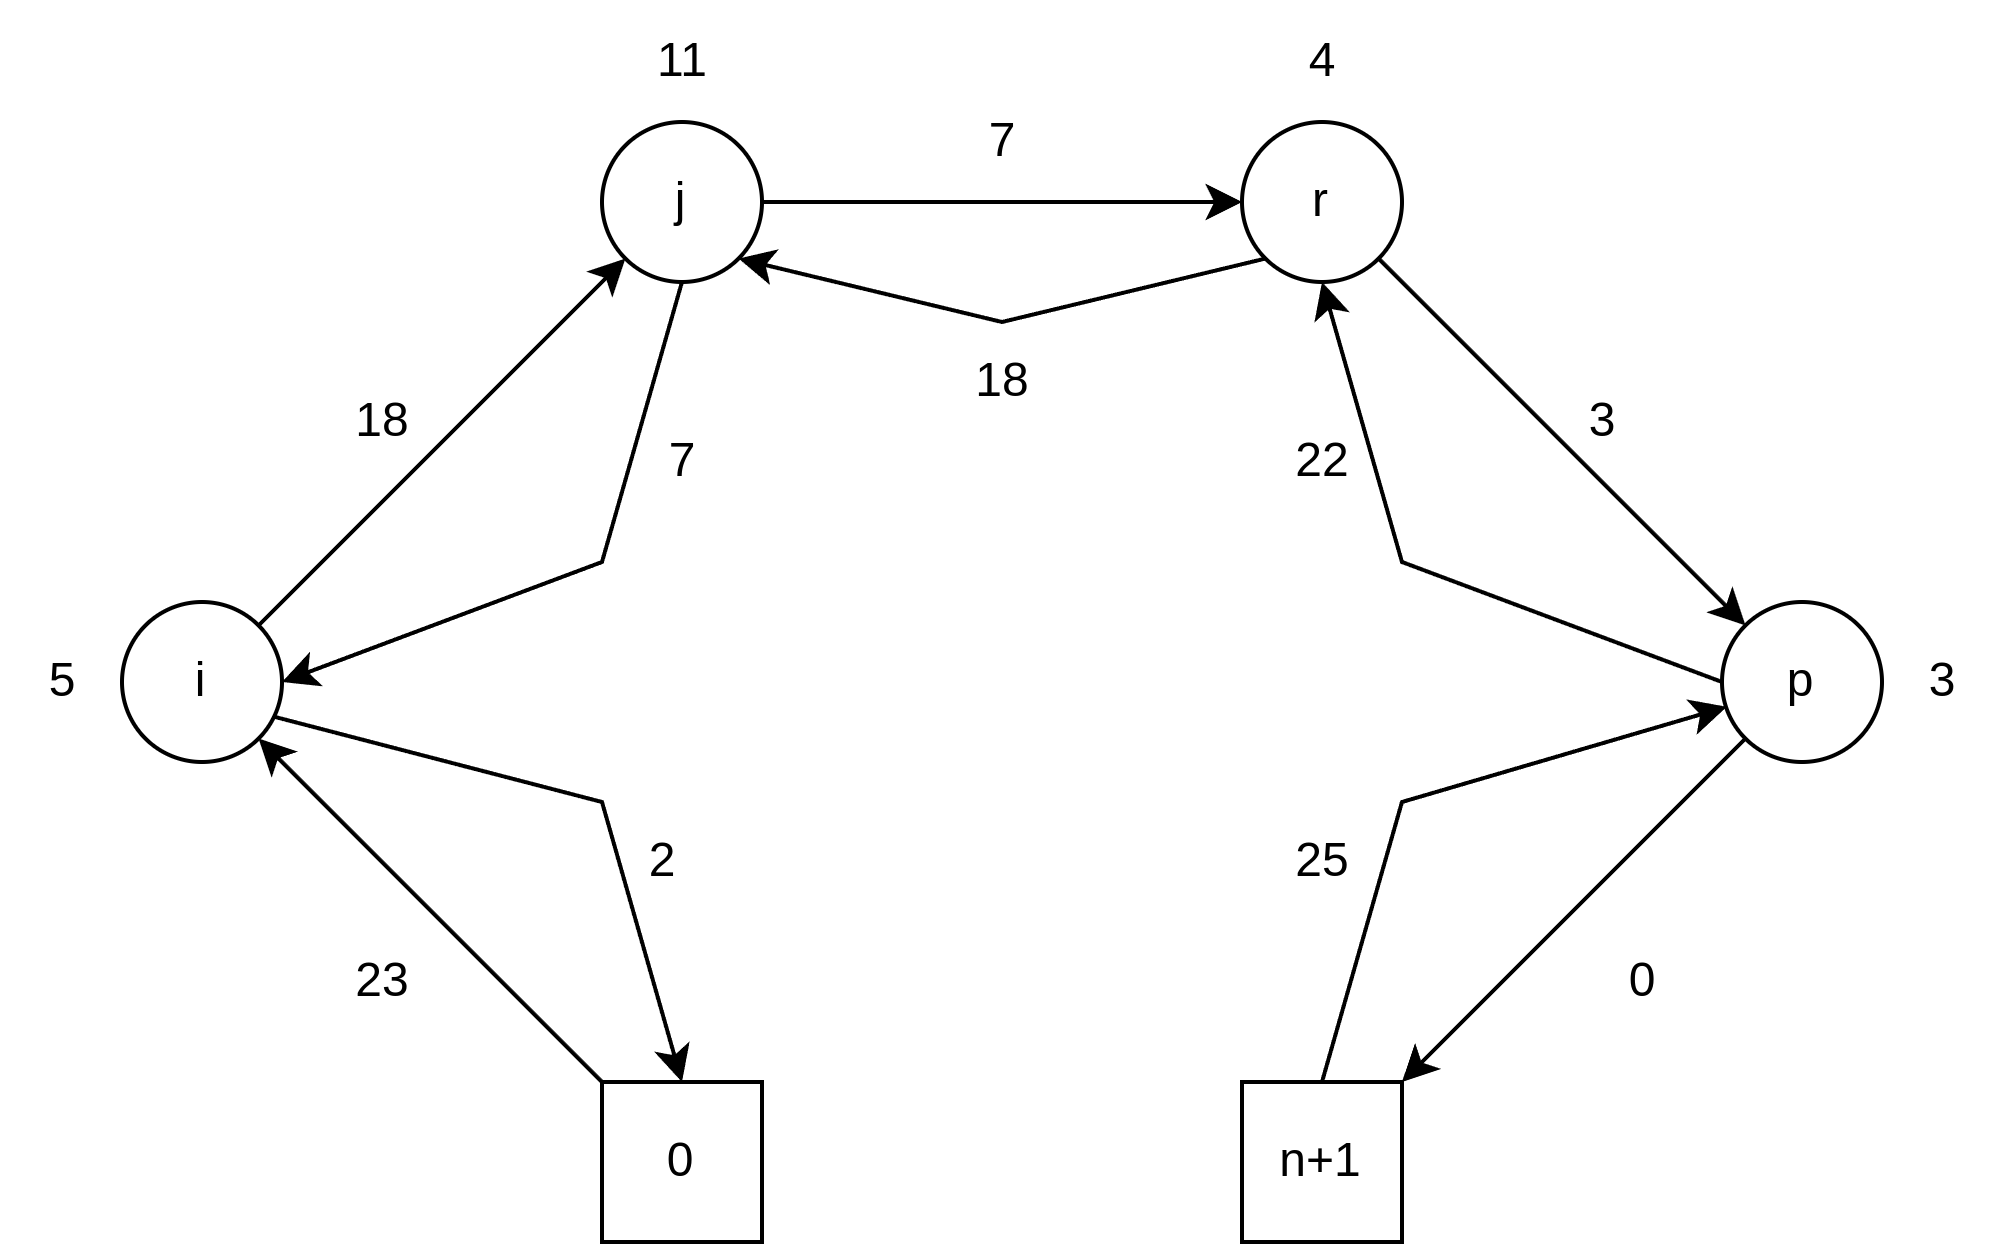
\includegraphics[width=0.8\textwidth]{figures/commondity-flow-model.png} 
  % \includesvg[scale=1]{figures/core-object}
  \caption{Minh họa dòng hàng với $Q=25$} 
  % \label{fig:fg_02}
\end{figure}

\subsection{Công thức phân hoạch tập hợp và thuật toán}
Công thức phân hoạch tập hợp đơn giản của VRP lần đầu được nghiên cứu bởi Balinski, Quandt (1964) \cite{balinski1964integer}. Gọi $r$ là một tuyến, $a_{ir}$ là hệ số nhị phân có giá trị bằng $1$ khi và chỉ khi nút $i \in V \setminus \{0\}$ thuộc tuyến $r$, gọi $c^*$ là chi phí tối ưu của tuyến $r$ và gọi $y_k$ la biến nhị phân bằng $1$ khi và chỉ khi tuyến $r$ được dùng trong lời giải tối ưu. Bài toán được mô hình hóa như sau

\begin{equation}
	\min \sum_r{c_r^* y_r}
\end{equation}
s.t.
\begin{flalign}
	\label{ct4:1} & \sum_r a_{ir} = 1 & \quad (i \in V \setminus \{0\}), \\
	\label{ct4:2} & \sum_r y_r = m,   & \quad                            \\
	\label{ct4:3} & y_r = 0, 1        & \quad (\text{mọi } r).
\end{flalign}

Nói một cách chặt chẽ thì ràng buộc (\ref{ct4:2}) không phải một phần của công thức phân hoạch tập hợp chuẩn, tuy nhiên nó được sử dụng bởi hầu hết các nhà nghiên cứu trong trường hợp VRP.

\section{Heuristics cổ điển}

Nhìn chung thì các thuật toán giải chính xác khó đảm bảo hiệu năng trong thực tế khi mà các tập dữ liệu ngày các lớn và các doanh nghiệp cần phục vụ khách hàng một cách nhanh chóng và tiết kiệm. Thực tế người ta cần tìm ra một (số) lời giải chập nhận được đủ tốt trong một khoảng thời gian "hợp lý". Từ những năm 1964 cho đến 1990, rất nhiều heuristics được nghiên cứu. Một số ít là đưa ra thuật toán hoàn toàn mới còn hầu hết là cải tiến thuật toán đã có.

\subsection{Thuật toán tiết kiệm}

Thuật toán tiết kiệm được đưa ra bởi Clark, Wright (1964) \cite{clarke1964scheduling}, mô tả và cài đặt khá đơn giản nhưng vẫn đưa ra được nghiệm tốt. Chính vì thế, thuật toán này được sử dụng rất rộng rãi. Thuật toán bắt đầu với nghiệm ban đầu với $n$ tuyến $(0, i, 0)$ với $i \in V \setminus \{0\}$. Tại mỗi vòng lặp thuật toán nối tuyến kết thúc với $i$ với một tuyến khác bắt đầu với $j$ cực đại hóa đại lượng \textit{tiết kiệm} $s_{ij}=c_{i0} + c_{0j} - c_{ij}$ và lới giải mới thỏa mãn các ràng buộc. Quá trình kết thúc khi không thể nối các tuyến vào nữa.

Một số cải tiến được đề xuất, ví dụ như nhân $c_{ij}$ với một trọng số dương $\lambda$ (Golden, Magnanti, Nguyen (1977) \cite{golden1977implementing}), tối ưu tuyến đường hợp nhất toàn cục thông qua việc sử dụng thuật toán phù hợp (Altinkemer, Gavish (1991) \cite{altinkemer1991parallel} và Wark, Holt (1994) \cite{wark1994repeated}), tăng tốc tính toán (Paessens (1988) \cite{paessens1988savings})...

\subsection{Phân cụm trước, định tuyến sau}

Heuristic phân cụm trước, định tuyến sau của Fisher, Jaikumar (1981) \cite{fisher1981generalized} trước hết đặt $m$ tâm và phân cụm sao cho tổng khoảng cách từ các nút đến tâm của nó là nhỏ nhất và thỏa mãn về ràng buộc tải trọng. Sau đó trên mỗi cụm, tuyến đường được thiết lập bằng cách giải bài toán TSP. Một vài chiến thuật để khởi tạo cũng như lựa chọn tâm cụm được trình bày trong Baker, Sheasby (1999) \cite{baker1999extensions}

\subsection{Heuristics cải tiến}

\section{Metaheuristics}

Metaheuristics có thể được phân lọai thành tìm kiếm lân cận, tìm kiếm phổ biến và cơ chế học. Hầu hết các thuật toán metaheuristics cho VRP đều dựa trên tìm kiếm lân cận và là các phương pháp cải tiến. Các thuật toán tốt nhất khá mạnh mẽ ngay cả khi nghiệm khởi tạo có chất lượng thấp. Một xu hướng chung là thay vì sử dụng chỉ một thuật toán, người ta thường kết hợp nhiều thuật toán lại với nhau. Các thuật toán như vậy được gọi là thuật toán lai.

Tiếp theo tác giả trình bày ý tưởng chính của một số lớp thuật toán metaheurictics.

\subsection{Tìm kiếm cục bộ}

Về cơ bản, tìm kiếm lân cận cố gắng "khám phá" không gian nghiệm bằng cách "di chuyển" quanh nghiệm hiện tại tới một nghiệm khác trong vùng lần cận của nó. Một số phương pháp có thể kể đến như \textit{tabu search} (Glover (1986) \cite{glover1986future}), \textit{simulated annealing} (Kirkpatrick, Gelatt, and Vecchi
(1983) \cite{kirkpatrick1983optimization}), \textit{deterministic annealing} (Dueck, Scheurer
(1990) \cite{dueck1990threshold}; Dueck (1993) \cite{dueck1993new}), \textit{variable neighbourhood search} (Mladenović, Hansen (1997) \cite{mladenovic1997variable}), \textit{large neighbourhood search}(Shaw (1998) \cite{shaw1998using}) và \textit{adaptive large neighbourhood search} (Ropke, Pisinger (2006) \cite{ropke2006adaptive}). Các thành phần chính của tìm kiếm lân cận là các quy tắc để xác định vùng lân cận của một nghiệm và cơ chế để khám phá vùng lân cận đó.

Trong \textit{tabu search} không gian nghiệm được khám phá bằng cách di chuyển từ nghiệm hiện tại đến nghiệm tốt nhất trong một tập con của lân cận của nghiệm đó. Để tránh việc lặp lại các nghiệm, các nghiệm được gán một thuộc tính gắn với nghiệm hiện tại để không được chọn trong một số lần lặp tiếp theo. Một nghiệm trở thành nghiệm tốt nhất trong số các nghiệm đã biết có thuộc tính gắn với thuộc tính hiện tại. Nguyên lý này được trình bày đầu tiên bởi Cordeau, Gendreau, Laporte (1997) \cite{cordeau1997tabu} và hiện nay được biết đến như là phương pháp tìm kiếm dựa trên thuộc tính (Derigs, Kaiser (2007) \cite{derigs2007applying}).

Trong \textit{simulated annealing} một gnhiệm $x$ được chọn ngẫu nhiên trong lân cận $N(x_t)$ của nghiệm hiện tại $x_t$ tại vòng lặp $t$. Nếu hàm mục tiêu $f$ cực tiểu, ta gán $x_{t+1}:=x$ với $f(x_{t+1}) \leq f(x_t)$. Ngược lại gán $x_{t+1}:=x$ với một xác suất $p_t$ và gán $x_{t+1}:=x_t$ với xác suất $1-p_t$. Trong đó, $p_t$ là một hàm giảm theo $t$ và $f(x) - f(x_t)$.

Trong \textit{deterministic annealing}, nghiệm $x$ cũng được chọn ngẫu nhiên trong lân cận $N(x_t)$. Trong thuật toán \textit{threshold-accepting} (Dueck, Scheurer (1990) \cite{dueck1990threshold}), $x_{t+1}:=x$ khi $f(x) < f(x_t) + \theta_1$, với $\theta_1$ là một trọng số dương; ngược lại gán $x_{t+1}:=x_t$. Trong \textit{record-to-record travel} (Dueck (1993) \cite{dueck1993new}), với nghiệm tốt nhất hiện tại $x^*$, gán $x_{t+1}:=x$ nếu $f(x) \leq \theta_2 f(x^*)$, với $\theta_2$ là một trọng số dương; ngược lại gán $x_{t+1}:=x_t$.; ngược lại gán $x_{t+1}=x_t$.

Trong \textit{Variable neighbourhood search} (Mladenović, Hansen (1997) \cite{}), tác giả xem xét một dánh sách được sắp xếp của các lân cận. Thuật toán bắt đầu với một lân cận và chuyển qua lân cận tiếp theo cho đến khi đạt tới nghiệm tối ưu cục bộ. Việc tìm kiếm được khởi tạo lại khi một nghiệm tốt hơn được tìm thấy hoặc tất cả các lân cận đã dược xét qua. \textit{Very large-scale neighbourhood search - LNS} bỏ đi và tạo lại một (vài) phần của nghiệm hiện tại để tìm kiếm nghiệm tốt hơn. Nguyên lí này giống như cơ chế hủy và tạo lại được trình bày bởi Shaw (1998) \cite{shaw1998using}. \textit{Adaptive large neighbourhood search - ALNS} (Ropke, Pisinger (2006) \cite{ropke2006adaptive}) được biết đến như là một phiên bản mạnh mẽ hơn của \textit{large neighbourhood search}, trong đó các thuật toán hủy hay tạo lại được lựa chọn một cách linh hoạt và thích ứng với trạng thái hiện tại của hệ. LNS và ALNS là cảm hứng chính cho luận văn này. Trong các phần tiếp theo tác giả sẽ trình bày chi tiết về ALNS.

\subsection{Tìm kiếm quần thể}

Tìm kiếm quần thể hoạt động với một quần thể các nghiệm. Thuật toán di truyền (Holland (1975) \cite{holland1975adaptation}) là ví dụ tốt nhất cho mô hình này. Tại mỗi vòng lặp, một vài nghiệm cha dược trích xuất từ quần thể hiện tại và kết hợp để tạo ra các nghiệm con. Nghiệm con sau đó được thay bằng những phần tệ nhất trong quần thể nếu điều này cải thiện nghiệm tốt nhất hiện tại. Về cơ bản, thuật toán áp dụng đa dạng hóa các cơ chế, gọi là đột biến cho thế hệ nghiệm con trước khi xem xét việc đưa chúng vào quần thể.


\subsection{Cơ chế học}

Cơ chế học vay mượn ý tưởng từ trí tuệ nhân tạo với mạng thần kinh (neural networks). Thuật toán học hỏi kinh nghiệm và điều chỉnh các trọng số qua các vòng lặp. Ứng dụng với VRP được trình bày bởi Ghaziri (1991) \cite{ghaziri1991solving}; Schumann, Retzko (1995) \cite{schumann1995self}. Thuật toán tối ưu đàn kiến cũng là một dạng khác của cơ chế học. Nó bắt chước hành vi của đàn kiến trong việc tìm thức ăn và để lại vết trên đường đi. Theo thời gian, vết được để lại nhiều hơn trên đường đi ngắn nhất và qua đó, kiến đi theo con đường này. Ứng dụng đầy đủ được trình bày bởi Reimann, Doerner, Hartl (2004) \cite{reimann2004d}



        \chapter{Phương pháp tìm kiếm lân cận}
\label{chap:search}

Như đã trình bày trong chương \ref{chap:solution}, hầu hết các thuật toán hiện đại đều dựa trên tìm kiếm lân cận và thuộc lớp cải tiến. Thuật toán không cố gắng để đưa ra ngay một nghiệm tối ưu ngay từ đầu (hay chỉ với một bước chạy). Thay vào đó, ta xuất phát từ một nghiệm chấp nhận được (thường được khởi tạo nhanh như thuật toán tham lam chẳng hạn), sau đó qua mỗi vòng lặp, nghiệm được cải thiện dần cho đến khi điều kiện dừng được thỏa mãn. Tại mỗi vòng lặp, thuật toán cố gắng khám phá không gian nghiệm bằng cách xét các lân cận của nghiệm hiện tại để tìm một nghiệm tối ưu địa phương. 

Chiến thuật này cần ta định nghĩa rõ ràng khái niệm "lân cận", "tối ưu địa phương", "tiêu chí chấp nhận nghiệm" và "điều kiện dừng". Lân cận được hiểu là một nghiệm chấp nhận được (theo nghĩa thỏa mãn các ràng buộc) với một thay đổi không quá lớn từ nghiệm hiện tại. Ví dụ, một vài yêu cầu từ tuyến này được trao đổi với tuyến khác hoặc được chuyển hẳn sang một tuyến khác hay là tạo một tuyến mới. Nghiệm tối ưu địa phương là nghiệm tốt nhất ta có thể tìm được trong lân cận như vậy. Tuy nhiên, nếu ta tiếp tục tìm kiếm từ nghiệm tối ưu địa phương thì đôi khi thuật toán bị "mắc" tại nghiệm đó. Cụ thể hơn, thuật toán trải qua nhiều vòng lặp mà chỉ xét các nghiệm lân cận của một tối ưu địa phương hoặc độ cải thiện là rất chậm. Chính vì vậy, có nhiều tiêu chí chấp nhận hay tiêu chí lựa chọn nghiệm để thuật toán thoát khỏi vùng này được phát triển thay vì chỉ chấp nhận nghiệm có chi phí nhỏ nhất trong lân cận. Một vài tiêu chí có thể kể đến như \textit{tìm kiếm tabu} (\textit{tabu search}), \textit{mô phỏng luyện kim} (\textit{simulated annealing}), \textit{chấp nhận với ngưỡng} (\textit{threshold-accepting}) hay \textit{duyệt qua bản ghi} (\textit{record-to-record travel}) đã được trình bày ở chương trước. Nhìn chung, thay vì tiếp tục tìm kiếm từ một tối ưu địa phương, chúng ta đưa vào hàm mục tiêu một hệ số phạt (nhỏ) nào đó để có thể tìm kiếm từ một nghiệm tệ hơn nghiệm tối ưu địa phương một chút. Điều kiện dừng thường được áp dụng là số vòng lặp tối đa hoặc thời gian tối đa mà thuật toán được phép chạy. Thời gian này thường được gọi là \textit{timeout}.

\section{Tìm kiếm lân cận rộng}
\section{Tìm kiếm lân cận rộng thích ứng}
Tìm kiếm lân cận rộng thích ứng (\textit{adaptive large neighbourhood search - ALNS}) được giới thiệu bởi S. Ropke và D. Pisinger \cite{ropke2006adaptive} là một mở rộng của LNS. Thay vì chỉ sử dụng một chiến thuật hủy và một chiến thuật thêm lại yêu cầu như LNS, ALNS cho phép lựa chọn nhiều toán tử hủy và thêm lại. Việc này cho phép thuật toán tìm kiếm không gian nghiệm một cách linh hoạt hơn và khó bị bẫy ở một nghiệm tối ưu cục bộ. Điểm thú vị của ALNS là các thuật toán hủy và thêm lại không được chọn một cách ngẫu nhiên mà lựa chọn có trọng số phụ thuộc vào trạng thái (nghiệm hiện tại) của bài toán.

\subsection{Lựa chọn phương pháp xóa và thêm lại}
Để lựa chọn phương pháp xóa và thêm lại, ta gán cho mỗi heuristic một trọng số khác nhau và sử dụng nguyên tắc "bánh xe lựa chọn". Nếu có $k$ heuristic với trọng số $w_i, i \in \{1,...,k\}$, ta chọn heuristic $j$ với xác suất
\begin{equation}
	\label{eq:select}
	p_j = \frac{w_j}{\sum_{i=1}^k w_i}.
\end{equation}
Lưu ý rằng, việc lựa chọn thuật toán xóa và thêm lại là độc lập với nhau. Các trọng số này có thể được thiết lập thủ công và không đổi trong suốt vòng đời của việc tìm kiếm hoặc nó có thể được điều chỉnh tự động để "thích ứng" với trạng thái hiện tại của hệ. Một cách điều chỉnh các tham số này tự động được trình bày ngay sau đây.

\subsection{Điều chỉnh tham số tự động}
Trọng số được điều chỉnh mỗi khi có nghiệm mới được chấp nhận. Ý tưởng chung là theo dõi một điểm số đại diện cho độ hiệu quả của thuật toán trong các vòng lặp gần đây. Điểm số càng cao thì thuật toán được chọn càng hiệu quả. Quá trình tìm kiếm được chia thành nhiều bước, mỗi bước là một số vòng lặp. Điểm của mỗi heuristic được đặt là $0$ khi bắt đầu và được tăng thêm $\sigma_1, \sigma_2, \sigma_3$ tùy thuộc vào tình huống.
\begin{table}[caption={Tham số cập nhật trọng số.}, label=tab:weight]
	\begin{tabularx}{\textwidth}{|l|X|}
		\hline
		Tham số    & Mô tả  \\ \hline
		$\sigma_1$ & Hành động xóa-chèn cuối cùng dẫn đến một nghiệm mới tốt hơn nghiệm tốt nhất toàn cục. \\ \hline
		$\sigma_2$ & Hành động xóa-chèn cuối cùng dẫn đến một nghiệm mới có chi phí tốt hơn chi phí của nghiệm hiện tại. \\ \hline
		$\sigma_3$ & Hành động xóa-chèn cuối cùng dẫn đến một nghiệm mới có chi phí tệ hơn chi phí của nghiệm hiện tại nhưng thỏa mãn điều kiện chấp nhận nghiệm. \\ \hline
	\end{tabularx}
\end{table}

Trong mỗi bước, thao tác xóa và thêm lại được cập nhật một lượng như nhau vì ta không chắc sự "cải thiện" nghiệm đến từ việc xóa hay thêm lại yêu cầu. Mỗi khi kết thúc bước, ta tính toán lại trọng số mới sử dụng các điểm số trên. Gọi $\omega_{ij}$ là trọng số của heuristic $i$ trong bước $j$. Ta đánh các trọng số như nhau tại bước đầu tiên, sau đó khi bước $j$ kết thúc, ta tính lại trọng số cho tất cả các heuristic để sử dụng cho bước $j+1$ như sau
\begin{equation}
	\label{eq:adaptive_weight}
	\omega_{i, j+1} = \omega_{ij}(1-r)+r\frac{\pi_i}{\theta_i}.
\end{equation}
Trong đó $\pi_i$ là điểm số của heuristic $i$ trong bước $j$ và $\theta_i$ là số lần ta cố gắng sử dụng heuristic $i$ trong bước $j$. Tham số $r$ là tham số điều khiển tốc độ điều chỉnh trọng số (được đặt mặc định bằng $0.1$ trong thực nghiệm). Nếu $r=0$, nghĩa là chúng ta không sử dụng điểm để điều chỉnh trọng số hay nói cách khác là các trọng số được giữ nguyên từ trong suốt quá trình tìm kiếm. Nếu $r=1$, nghĩa là ta lấy điểm thu được từ bước gần nhất để quyết định trọng số.

Việc điều chỉnh trọng số như trên làm tăng xác suất chọn thuật toán xóa (chèn) đã mang lại hiệu quả ở bước trước đó. Về cơ bản, với việc sử dụng chiến thuật điều chỉnh trọng số như trên, ta kì vọng rằng các thuật toán xóa (chèn) đã hiệu quả ở bước trước thì cũng sẽ hiệu quả ở bước tiếp theo. Trong thực nghiệm, các tham số được lựa chọn lần lượt là $\sigma_1=10$, $\sigma_2=4$ và $\sigma_3=2$.

\subsection{Thêm nhiễu khi chỉnh tham số tự động}
Như đã trình bày, với việc sử dụng chiến thuật lựa chọn tham số tự động như trên, ta kì vọng rằng thuật toán nếu đang hiệu quả thì nó sẽ tiếp tục hiệu quả. Tuy nhiên việc cộng một lượng cố định vào thuật toán đó về lâu dài (khi trải qua nhiều vòng lặp) thì trọng số của nó trở lên lớn dẫn đến xác suất lựa chọn thuật toán này cũng lớn theo. Chúng ta cũng chưa sử dụng yếu tố vòng lặp (hay thời gian chạy). Do đó, tác giả đề xuất ý tưởng đơn giản là nếu rất "lâu" rồi ta mới có một thuật toán hiệu quả thì ta cũng nên điều chỉnh trọng số của nó theo "thời gian chờ đó". Giả sử sau $m$ vòng lặp, chúng ta mới lại có một nghiệm được chấp nhận từ lần cuối cùng nghiệm được chấp nhận, trọng số của thuật toán sẽ được điều chỉnh một lượng tỉ lệ với $1 - e^{-\gamma m}$. Hàm $\text{exp}$ được sử dụng để chuẩn hóa lượng này trong khoảng $(0,1)$ khi $m$ lớn hoặc nhỏ. Cuối cùng ta có biểu thức cho trọng số của thuật toán như sau
\begin{equation}
	\label{eq:boost_adaptive_weight}
	\omega_{i, j+1} = \omega_{ij}(1-r)+r\frac{\pi_i} {\theta_i} + \alpha \beta (1 - e^{-\gamma m})
\end{equation}
với $\alpha$ (có thể âm hoặc dương) và $\gamma$ (dương) là các tham số điều khiển, $\beta$ là một số ngẫu nhiên trong khoảng $(0,1)$ \footnote[1]{Trong thực nghiệm, các tham số được đặt mặc định $\alpha = -1$, $\gamma = 1$. Ta có thể điều chỉnh các tham số này tùy thuộc vào bài toán để thu được kết quả tốt nhất.}. Trong phần thực nghiệm \ref{sec:performance}, tác giả sẽ chỉ ra sự vượt trội về hiệu năng khi thêm nhiễu vào việc điều chỉnh trọng số như trên. Chính vì vậy, thuật toán được đặt tên là B-ALNS (\textit{Boosted - Adaptive Large Neighborhood Search}).

\subsection{Số lượng yêu cầu bỏ đi và thêm lại}
\label{sec:num_rm_req}
Số lượng yêu cầu bỏ đi và thêm lại trong mỗi vòng lặp là một tham số quan trọng. Nếu số lượng yêu cầu bỏ đi và thêm lại quá ít, thuật toán sẽ không thể khám phá được không gian nghiệm một cách đủ lớn. Nếu số lượng yêu cầu bỏ đi và thêm lại quá nhiều, thuật toán sẽ tốn nhiều thời gian tính toán và không thể tìm được nghiệm tốt trong thời gian hợp lý. Việc lựa chọn một con số phù hợp với kích thước của cấu hình (đầu vào) và tài nguyên của máy tính không đơn giản. Trong thực nghiệm, tác giả đã thử nghiệm với nhiều con số khác nhau và nhận thấy rằng, việc sử dụng một lượng yêu cầu bỏ đi và thêm lại ngẫu nhiên trong một khoảng nhất định (phụ thuộc vào kích thước cấu hình) thu được chất lượng nghiệm cũng như hiệu năng tổng thể tốt hơn so với việc chỉ sử dụng một con số cố định. Số yêu cầu được bỏ đi thường không vượt quá $10\%$ kích thước cấu hình theo D. Pisinger và S. Ropke \cite{pisinger2007general}. Đối với các cấu hình kích thước lớn, số lượng yêu cầu bỏ đi nằm trong khoảng từ 30 đến 60.
        \chapter{Ứng dụng ALNS vào CVRPTW}

\begin{figure}[H] % places figure environment here   
  \centering % Centers Graphic
  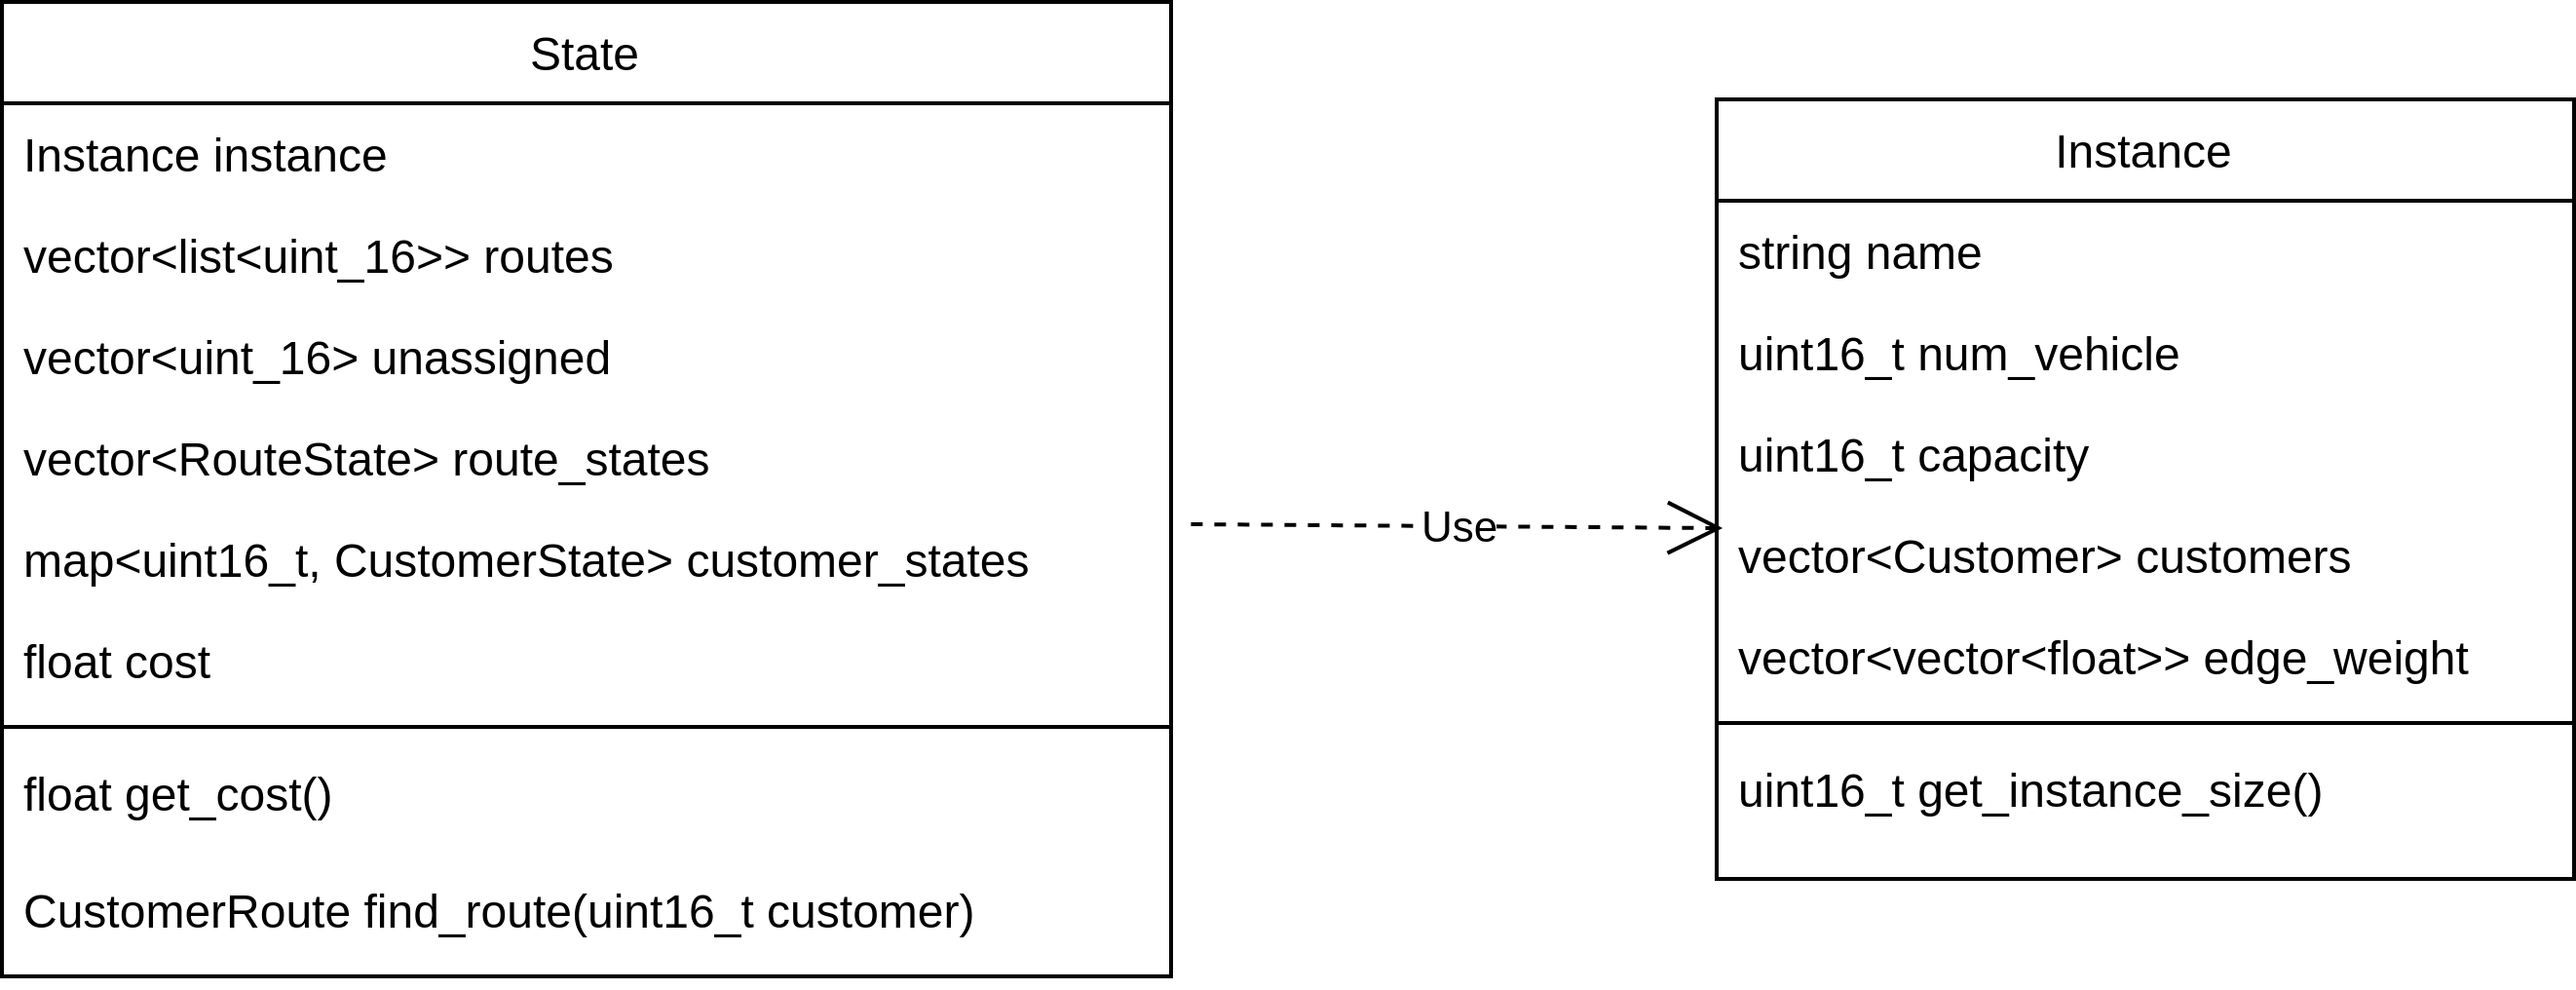
\includegraphics[width=1\textwidth]{figures/core-object.png} 
  % \includesvg[scale=1]{figures/core-object}
  \caption{Đối tượng chính của chương trình} 
  \label{fig:fg_02}
\end{figure}
        \chapter{Thực nghiệm và kết quả}

Trong phần này, chúng ta sẽ xem xét kết quả thực nghiệm thu được khi áp dụng ALNS cho VRPTW với hai tập dữ liệu của Solomon (1987) và Homberger \& Gehring (1999). Ở cả hai tập, các bộ dữ liệu được chia thành 3 loại C, R và RC. Với dữ liệu lớp C, các yêu cầu được phân thành các cụm rõ rệt, lớp R là hoàn toàn ngẫu nhiên và lớp RC là sự kết hợp của hai lớp trên. Tác giả chỉ xem xét các tập từ 100 yêu cầu trở lên (bỏ qua tập Solomon 25, 50 yêu cầu vì nhìn chung số lượng yêu cầu như vậy là quá nhỏ để nhận thấy sự khác biệt khi so sánh ALNS với các thuật toán khác).

\begin{figure}[H] % places figure environment here   
	\label{fig:perf_ct_c1}
	\begin{subfigure}{.3\textwidth}
		\centering
		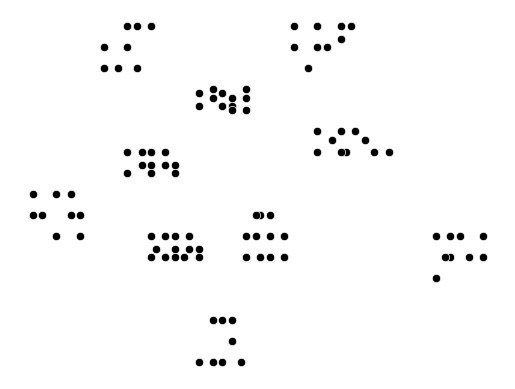
\includegraphics[width=1\linewidth]{figures/cls_c.png}
		\caption{C-class}
		\label{fig:cls_c}
	\end{subfigure}%
	\begin{subfigure}{.3\textwidth}
		\centering
		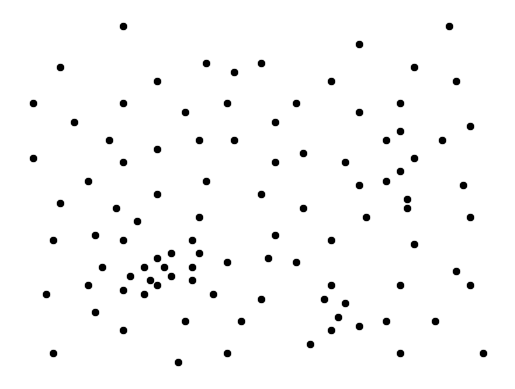
\includegraphics[width=1\linewidth]{figures/cls_r.png}
		\caption{R-class}
		\label{fig:cls_r}
	\end{subfigure}
	\begin{subfigure}{.3\textwidth}
		\centering
		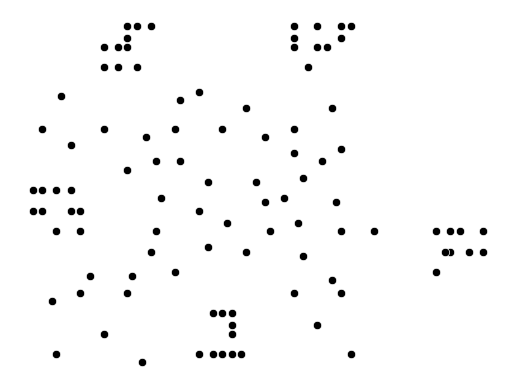
\includegraphics[width=1\linewidth]{figures/cls_rc.png}
		\caption{RC-class}
		\label{fig:cls_rc}
	\end{subfigure}
	\caption{Lớp các cấu hình}
\end{figure}

\begin{figure}[H] % places figure environment here   
	\label{fig:perf_ct_c1}
	\begin{subfigure}{.3\textwidth}
		\centering
		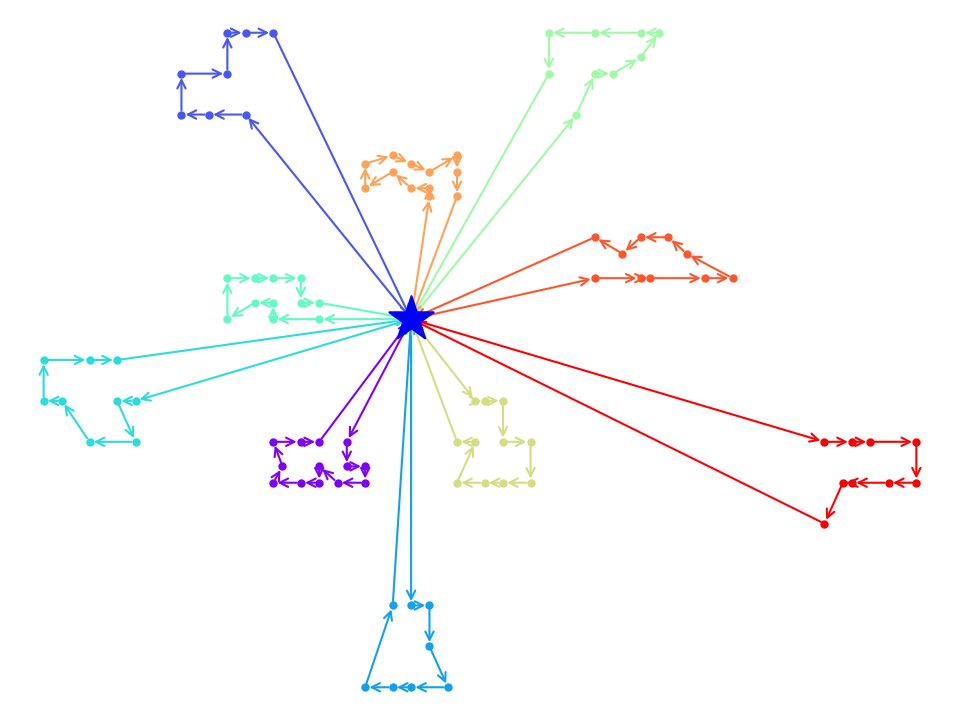
\includegraphics[width=1\linewidth]{figures/routes_c101.png}
		\caption{C-class}
		\label{fig:route_c}
	\end{subfigure}%
	\begin{subfigure}{.3\textwidth}
		\centering
		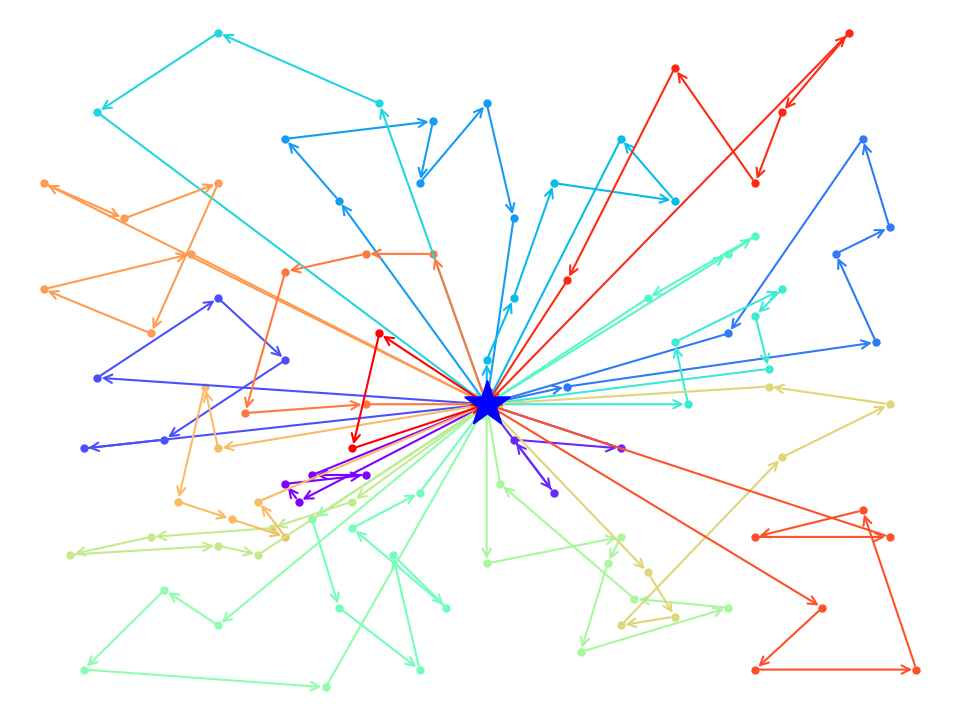
\includegraphics[width=1\linewidth]{figures/routes_r101.png}
		\caption{R-class}
		\label{fig:route_r}
	\end{subfigure}
	\begin{subfigure}{.3\textwidth}
		\centering
		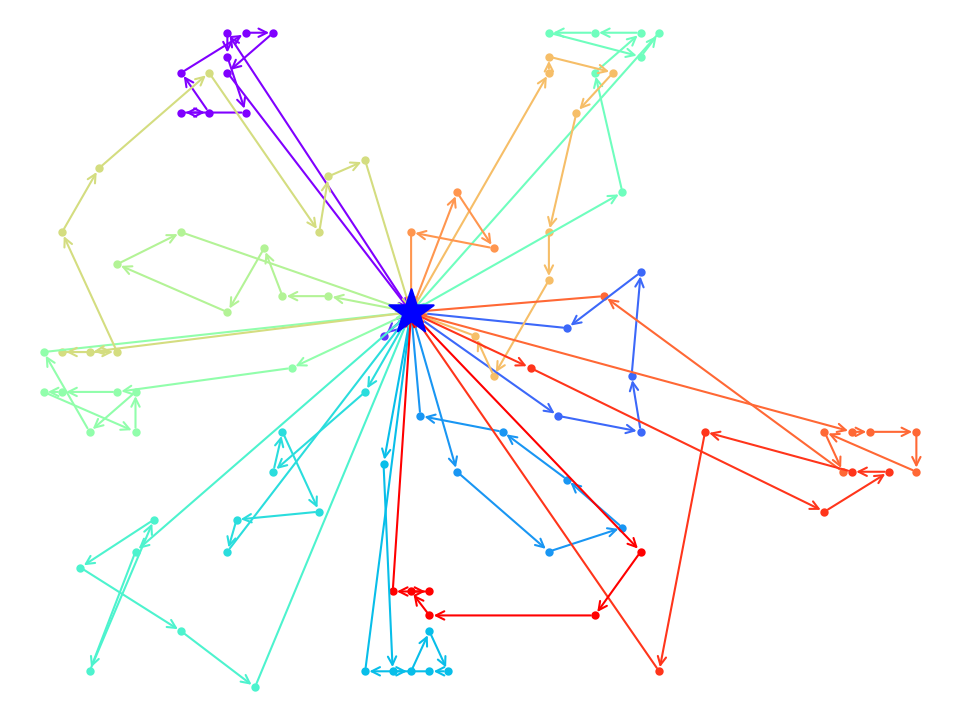
\includegraphics[width=1\linewidth]{figures/routes_rc101.png}
		\caption{RC-class}
		\label{fig:route_rc}
	\end{subfigure}
	\caption{Minh họa lời giải cho các lớp cấu hình}
\end{figure}

Tất cả các thí nghiệm được chạy trên CPU Intel(R) Xeon(R) CPU E5-2680 v4 @ 2.40GHz với Ubuntu 22.04.1 LTS. Mã nguồn được viết bằng ngôn ngữ C++ và được biên dịch bằng GCC 11.4.0 với các tùy chọn tối ưu hóa -O3.

\section{Chất lượng nghiệm}

Trong phần này, tác giả đưa ra các số liệu thực nghiệm về giá trị hàm mục tiêu khi áp dụng ALNS giải VRPTW. Do thuật toán sử dụng rất nhiều tham số ngẫu nhiên nên chúng ta không tiến hành chạy một lần mà chạy nhiều lần để thu được kết quả tốt nhất cũng như kết quả trung bình và đánh giá độ ổn định của thuật toán. Độ ổn định được đánh giá bằng độ lệch chuẩn của các kết quả đo giá trị hàm mục tiêu. Thực tế số lần chạy không quá lớn do thời gian chạy mỗi cấu hình là khá lâu nhưng tác giả vẫn cố gắng đưa vào độ đo độ lệch chuẩn để phần nào đánh giá được độ ổn định của thuật toán. Về mặt thống kê, điều này chưa hẳn là đúng đắn tuy nhiên ta vẫn thấy được một phần sự ổn định của ALNS qua các kết quả đo được. Số xe được sử dụng cũng được tác giả chỉ ra. Ta biết rằng số xe sử dụng ảnh hưởng rất nhiều đến hàm mục tiêu. Về cơ bản, khi có quá nhiều xe được sử dụng thì chất lượng nghiệm là tệ. Lâu dài, khi hàm mục tiêu "gần" hơn với giá trị tối ưu thì số xe cũng ổn định ở một mức nào đó và nhìn chung là giảm so với nghiệm ban đầu (được khởi tạo). Các kết quả sau đó được so sánh với nghiệm tốt nhất đã biết được lấy từ trang CVRPLIB (\href{http://vrp.galgos.inf.puc-rio.br/index.php/en/}{http://vrp.galgos.inf.puc-rio.br/index.php/en/}). Sintef (\href{https://www.sintef.no/}{https://www.sintef.no/}) cũng là một nguồn được sử dụng khá rộng rãi trong các bài báo khoa học nhưng nghiệm được báo cáo có chất lượng không tốt bằng CVRPLIB. 

\subsection{Số lượng yêu cầu liệu nhỏ}
\label{sec:exp_small}

Trước tiên, chúng ta bắt đầu với tập dữ liệu Solomon (1987) được đưa ra bởi Solomon (1987) \cite{solomon1987algorithms}. Solomon (1987) là một tập dữ liệu nổi tiếng được sử dụng để đánh giá chất lượng trong hầu hết các nghiên cứu về VRP. Các cấu hình và nghiệm được định dạng tiêu chuẩn bao gồm tên cấu hình, số xe tối đa dược sử dụng, tải trọng mỗi xe, ID của yêu cầu, tọa độ của các yêu cầu, nhu cầu (về tải) của mỗi yêu cầu, khung thời gian và thời gian phục vụ tại mỗi yêu cầu. Thông tin về kho được cho bởi ID 0. Với các cấu hình theo tiêu chuẩn định dạng Solomon (kể cả các cấu hình khác ngoài Solomon (1987)), tốc độ của xe được hiểu là 1 đơn vị; nói cách khác, thời gian di chuyển giữa các yêu cầu bằng với khoảng các giữa chúng. 

Tập dữ liệu được chia thành 3 lớp C, R và RC. Solomon sinh hai tập loại 1 và loại 2. Quy tắc đặt tên \code{\{class\}\{type\}\{num\}} với \code{class} là lớp C, R hoặc RC, \code{type} là loại 1 hoặc 2, \code{num} là số thứ tự của cấu hình. Mỗi lớp có từ $8$ đến $12$ cấu hình. Các cấu hình cũng được chia thành ba nhóm với $25$, $50$ và $100$ yêu cầu. Trong luận văn này, tác giả chỉ đưa ra các kết quả cho các tập $100$ yêu cầu do các cấu hình $25$ hay $50$ yêu cầu là khá nhỏ và ta không thấy rõ sự khác biệt do hầu hết các thuật toán đều cho kết quả rất tốt.

\begin{table}[caption={Kết quả đo với tập Solomon C}, label=exp:solomonC]
  \begin{adjustbox}{width=1\textwidth}
  \small
  \begin{tabularx}{\textwidth}{|XXXXXX|XXXXXX|}
  \hline
  ins & cost & nv & bkcost & bknv & gap & ins & cost & nv & bkcost & bknv & gap \\ \hline
  c101 & 828.94 & 10 & 827.30 & 10 & 0.20 & c201 & 591.56 & 3 & 589.10 & 3 & 0.42 \\ \hline
  c102 & 828.94 & 10 & 827.30 & 10 & 0.20 & c202 & 591.56 & 3 & 589.10 & 3 & 0.42 \\ \hline
  c103 & 828.06 & 10 & 826.30 & 10 & 0.21 & c203 & 591.17 & 3 & 588.70 & 3 & 0.42 \\ \hline
  c104 & 824.78 & 10 & 822.90 & 10 & 0.23 & c204 & 590.60 & 3 & 588.10 & 3 & 0.42 \\ \hline
  c105 & 828.94 & 10 & 827.30 & 10 & 0.20 & c205 & 588.88 & 3 & 586.40 & 3 & 0.42 \\ \hline
  c106 & 828.94 & 10 & 827.30 & 10 & 0.20 & c206 & 588.49 & 3 & 586.00 & 3 & 0.43 \\ \hline
  c107 & 828.94 & 10 & 827.30 & 10 & 0.20 & c207 & 588.29 & 3 & 585.80 & 3 & 0.42 \\ \hline
  c108 & 828.94 & 10 & 827.30 & 10 & 0.20 & c208 & 588.32 & 3 & 585.80 & 3 & 0.43 \\ \hline
  c109 & 828.94 & 10 & 827.30 & 10 & 0.20 &  &  &  &  &  &  \\ \hline
  avg & & & & & 0.20 &  &  &  &  & & 0.42 \\ \hline
  \end{tabularx}
  \end{adjustbox}
  \end{table}

  \textit{ Trong đó
    \begin{itemize}
      \item[-] ins: cấu hình
      \item[-] cost: chi phí thu được với ALNS
      \item[-] nv: số xe được sử dụng
      \item[-] bkcost: chi phí tốt nhất đã biết
      \item[-] bknv: số xe tốt nhất đã biết
      \item[-] gap (\%): khoảng cách so với nghiệm tốt nhất đã biết
      \item[-] avg: trung bình cộng các giá trị theo cột tương ứng
    \end{itemize}
  }

  Với các cấu hình loại C, ALNS cho nghiệm cách nghiệm tốt nhất đã biết trung bình $0.20\%$ và $0.42\%$ cho C1 và C2. Trong thực tế, đối với các doanh nghiệp giao vận nhỏ, hoặc một nhóm người giao hàng thì số lượng yêu cầu như vậy là bình thường. Các nhóm giao hàng nhỏ thường nhận các yêu cầu được phân cụm một cách tương đối (theo khu vực địa lý) như vậy. 

  Thí nghiệm được thiết lập có thời gian timeout một phút, chạy năm lần và lấy kết quả tốt nhất. Tập C1 và C2 tương đối nhỏ và đã phân cụm nên trong thực tế thuật toán chạy rất nhanh để ra được nghiệm tốt và không có sự khác biệt giữa các lần chạy, trên CPU được thí nghiệm, ALNS mất dưới 1 giây để tìm ra nghiệm kém hơn nghiệm tốt nhất đã biết dưới $1\%$.

  \begin{table}[caption={Kết quả đo với tập Solomon R1}, label=exp:solomonR1]
    % \begin{adjustbox}{width=1\textwidth}
    \small
    \centering
    \begin{tabular}{lrrrll}
    \hline
    instance & alns best & nv & bkcost & bknv & gap (\%) \\ \hline
    r101 & 1,642.88 & 20 & 1,637.70 & 20 & 0.32 \\ \hline
    r102 & 1,472.81 & 18 & 1,466.60 & 18 & 0.42 \\ \hline
    r103 & 1,213.62 & 15 & 1,208.70 & 14 & 0.41 \\ \hline
    r104 & 976.61 & 11 & 971.50 & 11 & 0.53 \\ \hline
    r105 & 1,360.78 & 15 & 1,355.30 & 15 & 0.40 \\ \hline
    r106 & 1,239.37 & 13 & 1,234.60 & 13 & 0.39 \\ \hline
    r107 & 1,073.60 & 12 & 1,064.60 & 11 & 0.85 \\ \hline
    r108 & 944.44 & 10 & 932.10 & 10 & 1.32 \\ \hline
    r109 & 1,152.38 & 13 & 1,146.90 & 13 & 0.48 \\ \hline
    r110 & 1,078.59 & 12 & 1,068.00 & 12 & 0.99 \\ \hline
    r111 & 1,053.50 & 12 & 1,048.70 & 12 & 0.46 \\ \hline
    r112 & \text{955.68} & 10 & \text{948.60} & \text{10} & \text{0.75} \\ \hline
    avg &  &  &  &  & 0.61 \\ \hline
    \end{tabular}
    % \end{adjustbox}
  \end{table}

  Tập R1 và R2 có các yêu cầu được tạo hoàn toàn ngẫu nhiên thế nên cũng có nhiều nghiệm chấp nhận được và thuật toán cũng khó bị bẫy ở một nghiệm tối ưu địa phương. Tuy nhiên, thuật toán cũng mất nhiều thời gian để tìm nghiệm tối ưu hơn do có nhiều nghiệm thỏa mãn các ràng buộc. Riêng với tập R2, ALNS đã tìm ra nghiệm với số xe ít hơn nghiệm tốt nhất đã biết mà tổng khoảng cách chỉ chênh lệch nhỏ. Lớp R có thể được sử dụng để mô phỏng các yêu cầu ở những vùng thưa dân cư như nông thôn chẳng hạn. Các yêu cầu thưa thớt hơn ở thành phố và khoảng cách giữa các yêu cầu cũng không gần nhau (các yêu cầu không tập trung thành các cụm rõ rệt). Việc đặt số lượng lớn các bưu cục ở vùng nông thôn là không khả thi về mặt chi phí vận hành cho các doanh nghiệp. Như vậy, sử dụng một thuật toán tối ưu nào đó là tiết kiệm chi phí (quãng đường) rất nhiều so với việc giao hàng một cách ngẫu nhiên hay theo quy tắc "tham lam". 

  \begin{table}[caption={Kết quả đo với tập Solomon R2}, label=exp:solomonR2, placement=h]
    % \begin{adjustbox}{width=1\textwidth}
    \small
    \centering
    \begin{tabular}{lrrrll}
    \hline
    instance & alns best & nv & bkcost & bknv & gap (\%) \\ \hline
    r201 & 1,152.96 & \textbf{7} & 1,143.20 & 8 & 0.32 \\ \hline
    r202 & 1,035.32 & \textbf{7} & 1,029.60 & 8 & 0.42 \\ \hline
    r203 & 880.90 & 6 & 870.80 & 6 & 0.41 \\ \hline
    r204 & 743.91 & \textbf{4} & 731.30 & 5 & 0.53 \\ \hline
    r205 & 958.81 & 5 & 949.80 & 5 & 0.40 \\ \hline
    r206 & 883.92 & 5 & 875.90 & 5 & 0.39 \\ \hline
    r207 & 806.31 & 5 & 794.00 & 4 & 0.85 \\ \hline
    r208 & 948.57 & 4 & 701.00 & 4 & 1.77 \\ \hline
    r209 & 717.53 & 5 & 854.80 & 5 & 0.48 \\ \hline
    r210 & 909.32 & \textbf{5} & 900.50 & 6 & 0.99 \\ \hline
    r211 & 1,053.50 & 5 & 746.70 & 4 & 0.46 \\ \hline
    avg &  &  &  &  & 1.38 \\ \hline
    \end{tabular}
    % \end{adjustbox}
  \end{table}

  \begin{table}[caption={Kết quả đo với tập Solomon RC1}, label=exp:solomonRC1, placement=h]
    % \begin{adjustbox}{width=1\textwidth}
    \small
    \centering
    \begin{tabular}{rrrrrr}
    \hline
    instance & alns best & nv & bkcost & bknv & gap (\%) \\ \hline
    rc101 & 1,623.58 & 16 & 1,619.80 & 15 & 0.23 \\ \hline
    rc102 & 1,461.23 & 14 & 1,457.40 & 14 & 0.26 \\ \hline
    rc103 & 1,266.62 & 11 & 1,258.00 & 11 & 0.69 \\ \hline
    rc104 & 1,136.91 & 10 & 1,132.30 & 10 & 0.41 \\ \hline
    rc105 & 1,518.58 & 16 & 1,513.70 & 15 & 0.32 \\ \hline
    rc106 & 1,376.99 & 13 & 1,372.70 & 12 & 0.31 \\ \hline
    rc107 & 1,211.11 & 12 & 1,207.80 & 12 & 0.27 \\ \hline
    rc108 & 1,118.13 & 11 & 1,114.20 & 11 & 0.35 \\ \hline
    avg &  &  &  &  & 0.36 \\ \hline
    \end{tabular}
    % \end{adjustbox}
  \end{table}

  \begin{table}[caption={Kết quả đo với tập Solomon RC2}, label=exp:solomonRC2, placement=h]
    % \begin{adjustbox}{width=1\textwidth}
    \small
    \centering
    \begin{tabular}{rrrrrr}
    \hline
    instance & alns best & nv & bkcost & bknv & gap (\%) \\ \hline
    rc201 & 1,274.61 & \textbf{8} & 1,261.80 & 9 & 1.02 \\ \hline
    rc202 & 1,099.54 & \textbf{6} & 1,092.30 & 8 & 0.66 \\ \hline
    rc203 & 931.16 & 5 & 923.70 & 5 & 0.81 \\ \hline
    rc204 & 788.66 & 4 & 783.50 & 4 & 0.66 \\ \hline
    rc205 & 1,157.66 & 7 & 1,154.00 & 7 & 0.32 \\ \hline
    rc206 & 1,060.50 & \textbf{6} & 1,051.10 & 7 & 0.89 \\ \hline
    rc207 & 966.08 & 6 & 962.90 & 6 & 0.33 \\ \hline
    rc208 & 785.73 & 4 & 776.10 & 4 & 1.24 \\ \hline
    avg &  &  &  &  & 0.74 \\ \hline
    \end{tabular}
    % \end{adjustbox}
  \end{table}

  Tương tự như lớp R, ALNS vẫn thể hiện rất tốt cho cấu hình lớp RC khi cho khoảng cách trung bình so với nghiệm tốt nhất đã biết là $0.36\%$ và $0.74\%$ cho RC1 và RC2. Với một số cầu hình \code{rc201}, \code{rc202} và \code{rc206}, ALNS cũng tìm được nghiệm với số xe ít hơn so với nghiệm tốt nhất đã biết. Việc tiết kiệm được số xe về tổng thể là rất có ý nghĩa trong thực tế  bởi chi phí thuê hay mua xe, trả lương cho tài xế và vận hành... là lớn hơn nhiều so với khi tiết kiệm được một vài phần trăm về quãng đường. Tuy nhiên, với một số cấu hình \code{rc1}, ALNS sử dụng nhiều xe hơn.

  Nhìn chung, với tập dữ liệu dưới $100$ yêu cầu, ALNS luôn cho kết quả tốt với số xe cần sử dụng ít. Trong quá trình thực nhiệm, tác giả cũng nhận thấy các kết quả chênh lệch nhau rất ít giữa các lần chạy (dưới $1\%$). Như vậy, ta có thể đưa ra một nhận xét sớm rằng ALNS đáp ứng tốt cho các cấu hình VRPTW với số lượng yêu cầu nhỏ (dưới $100$ yêu cầu). Điều này gợi ý sử dụng ALNS cho các bài toán thực tế của doanh nghiệp nhỏ hoặc ít nhất là cho các bưu cục (ở các khu vực khác nhau) của các doanh nghiệp lớn.
  
  % Ngoài ra, ALNS chứng tỏ được sự ổn định và có hiệu năng đủ tốt (sẽ được trình bày ở phần \ref{sec:performance}) ngay cả với các cấu hình với số lượng yêu cầu rất lớn. Điều này gợi ý sử dụng ALNS cho các bài toán thực tế của doanh nghiệp nhỏ hoặc ít nhất là cho các bưu cục (ở các khu vực khác nhau) của các doanh nghiệp lớn. Mặc dù đã được đề xuất từ khá lâu (1987), nhưng tập Solomon (1987) vẫn chứng tỏ được giá trị của nó đối với các bài thí nghiệm hiện đại và có tính ứng dụng cao trong thực tế. Tác giả không đưa vào các kết quả trung bình của các lần chạy thuật toán và độ lệch chuẩn do tập dữ liệu khá nhỏ. Các độ đo này sẽ được trình bày trong phần tiếp theo với số lượng yêu cầu từ trung bình ($200$, $400$), lớn ($400$, $600$) và rất lớn ($800$, $1000$).

  \subsection{Số lượng yêu cầu lớn và rất lớn}
  \label{sec:exp_large}
  
  Trong phần này, tác giả tiến hành thực nghiệm ALNS với tập dữ liệu lớn hơn với số lượng yêu cầu từ $200$ lên tới $1000$. Về con số $1000$ so với $100$ không làm chúng ta cảm thấy sự khác biệt, nhưng lưu ý rằng, độ phức tạp của bài toán là giai thừa, $O(1000!)$ là một con số lớn khủng khiếp! Tập dữ liệu được sử dụng được sinh trong Gehring, Hermann, Homberger (1999) \cite{gehring1999parallel} (sau đây tác giả gọi là tập HG cho ngắn gọn). Các cấu hình được ghi theo tiêu chuẩn Solomon đã được trình bày trong phần \ref{sec:exp_small}. Quy tắc đặt tên được quy ước như sau \code{\{class\}\{type\}\_\{size\}\_\{num\}} với \code{class} là lớp cấu hình C, R hay RC; \code{type} là loại $1$ hoặc $2$ (tương tự như tập Solomon (1987), HG cũng được sinh 2 bộ dữ liệu); \code{size} là kích thước cấu hình (ví dụ $2$ là $200$ yêu cầu, $8$ là $800$ yêu cầu); \code{num} là số thứ tự của cấu hình.

  Với số lượng yêu cầu là 200, ALNS vẫn tỏ ra hiệu quả với thời gian timeout một phút. ALNS cho chênh lệch trung bình $0.23\%$, $1.60\%$ và $1.73\%$ lần lượt cho các lớp C, R, RC so với nghiệm tốt nhất đã biết. Ngoài ra, ALNS tỏ ra ổn định khi độ lệch chuẩn giữa các lần chạy là rất nhỏ khi so sánh với giá trị hàm mục tiêu. Số xe sử dụng cũng không có sự khác biệt so với nghiệm tốt nhất đã biết.

  Đối với tập 400 yêu cầu, ALNS cho kết quả không tốt như với các tập có số lượng yêu cầu nhỏ với thời gian timeout một phút. Độ chênh lệch trung bình lần lượt là $1.99\%$, $4.35\%$ và $5.78\%$ cho lớp C, R và RC khi so sánh với nghiệm tốt nhất đã biết. Ta có thể thấy rằng, đối với lớp khó như RC, ALNS không còn duy trì được hiệu quả như khi giải bài toán lớp C và R. Tuy nhiên, ALNS vẫn ổn định khi độ lệch chuẩn giữa các lần đo vẫn rất nhỏ so với giá trị hàm mục tiêu. 

  Dưới đây là các kết quả đo cho các cấu hình 200, 400, 600, 800 và 1000 yêu cầu cho 3 lớp C, R và RC. 

  \textit{Trong đó
  \begin{itemize}
    \item[-] ins: tên cấu hình
    \item[-] alns best: giá trị hàm mục tiêu tốt nhất đạt được bởi ALNS
    \item[-] alns avg: giá trị hàm mục tiêu trung bình (với 5 lần đo) đạt được bởi ALNS
    \item[-] alns std: độ lệch chuẩn của giá trị hàm mục tiêu (với 5 lần đo) đạt được bởi ALNS
    \item[-] nv: số xe được sử dụng bởi ALNS
    \item[-] bkcost: giá trị hàm mục tiêu tốt nhất đã biết
    \item[-] bknv: số xe được sử dụng bởi nghiệm tốt nhất đã biết
    \item[-] gap (\%): chênh lệch giữa giá trị hàm mục tiêu tốt nhất đạt được bởi ALNS và giá trị hàm mục tiêu tốt nhất đã biết
  \end{itemize}
  Thời gian timeout là một phút.
  }

  Nếu cho rằng việc chênh lệch chất lượng nghiệm so với nghiệm tốt nhất đã biết không vượt quá $10\%$ là đủ thì ALNS thể hiện tốt đối với các cấu hình từ $600$ yêu cầu trở xuống. Đối với các cấu hình có số lượng yêu cầu rất lớn như $800$ và $1000$ yêu cầu, ALNS cho nghiệm còn cách nghiệm tốt nhất đã biết khá xa (lớn hơn $10\%$ cho tập $1000$ yêu cầu) với timeout một phút. Con số một phút được lựa chọn để phù hợp với yêu cầu thực tế khi mà ta không thể chờ quá lâu để nhận được kết quả. Một chiến thuật khác là ta có thể lên lịch cho các xe vào ngày hôm trước để có các tuyến đường cho ngày hôm sau chẳng hạn (cho chương trình chạy "qua đêm", hay chạy với thời gian chờ lâu có thể là vài tiếng đồng hồ). Tác giả đã thử nghiệm và nhận thấy rằng, với thời gian chạy lâu hơn nữa (timeout mười phút) ALNS cho kết quả tốt hơn nhưng tốc độ giảm nghiệm là chậm (kéo khoảng cách với nghiệm tốt nhất đã biết giảm $1$ đến $2$ phần trăm), do càng gần với nghiệm tối ưu thì các tuyến đường khá khó để thay đổi nhất là đối với các cấu hình có số lượng yêu cầu quá lớn như vậy.
  
  \begin{table}[caption={Kết quả đo với tập HG\_C\_1\_2 200 yêu cầu}, label=exp:HGC12]
    % \begin{adjustbox}{width=1\textwidth}
      \small
      \centering
      \begin{tabular}{rrrrrrrr}
        \hline
        ins & alns best & alns avg & alns std & nv & bkcost & bknv & gap (\%) \\ \hline
        C1\_2\_1 & 2,704.57 & 2,704.57 & 0 & 20 & 2,698.6 & 20 & 0.22 \\ \hline
        C1\_2\_2 & 2,700.65 & 2,700.65 & 0 & 20 & 2,694.3 & 20 & 0.24 \\ \hline
        C1\_2\_3 & 2,682.18 & 2,711.28 & 45.2 & 20 & 2,675.8 & 20 & 0.24 \\ \hline
        C1\_2\_4 & 2,631.89 & 2,647.68 & 17.2 & 19 & 2,625.6 & 19 & 0.24 \\ \hline
        C1\_2\_5 & 2,702.05 & 2,711.04 & 17.99 & 20 & 2,694.9 & 20 & 0.27 \\ \hline
        C1\_2\_6 & 2,701.04 & 2,701.04 & 0 & 20 & 2,694.9 & 20 & 0.23 \\ \hline
        C1\_2\_7 & 2,701.04 & 2,701.04 & 0 & 20 & 2,694.9 & 20 & 0.23 \\ \hline
        C1\_2\_8 & 2,690.27 & 2,690.27 & 0 & 20 & 2,684 & 20 & 0.23 \\ \hline
        C1\_2\_9 & 2,645.47 & 2,650.42 & 9.9 & 19 & 2,639.6 & 19 & 0.22 \\ \hline
        C1\_2\_10 & 2,630.95 & 2,651.39 & 24.08 & 19 & 2,624.7 & 19 & 0.24 \\ \hline
        avg & 2,679.01 & 2,686.94 & 11.44 & & 2,672.73 & & 0.23 \\ \hline
      \end{tabular}
      % \end{adjustbox}
  \end{table}
    
  \begin{table}[caption={Kết quả đo với tập HG\_R\_1\_2 200 yêu cầu}, label=exp:HGR12]
    % \begin{adjustbox}{width=1\textwidth}
      \small
      \centering
      \begin{tabular}{rrrrrrrr}
        \hline
        ins & alns best & alns avg & alns std & nv & bkcost & bknv & gap (\%) \\ \hline
        R1\_2\_1 & 4,708.02 & 4,720.47 & 13.83 & 23 & 4,667.2 & 23 & 0.87 \\ \hline
        R1\_2\_2 & 4,011.45 & 4,029.16 & 12.06 & 20 & 3,919.9 & 20 & 2.34 \\ \hline
        R1\_2\_3 & 3,416.04 & 3,444.85 & 19.13 & 19 & 3,373.9 & 18 & 1.25 \\ \hline
        R1\_2\_4 & 3,121.85 & 3,146.43 & 15.45 & 19 & 3,047.6 & 18 & 2.44 \\ \hline
        R1\_2\_5 & 4,096.03 & 4,128.44 & 17.06 & 20 & 4,053.2 & 20 & 1.06 \\ \hline
        R1\_2\_6 & 3,588.31 & 3,626.85 & 22.15 & 20 & 3,559.1 & 19 & 0.82 \\ \hline
        R1\_2\_7 & 3,199.57 & 3,240.56 & 24.57 & 18 & 3,141.9 & 18 & 1.84 \\ \hline
        R1\_2\_8 & 2,973.75 & 3,006.53 & 18.22 & 18 & 2,938.4 & 18 & 1.2 \\ \hline
        R1\_2\_9 & 3,784.88 & 3,816.64 & 31.13 & 20 & 3,734.7 & 19 & 1.34 \\ \hline
        R1\_2\_10 & 3,385.86 & 3,416.78 & 29.63 & 19 & 3,293.1 & 18 & 2.82 \\ \hline
        avg & 3,628.58 & 3,657.67 & 20.33 & & 3,572.90 & & 1.60 \\ \hline
      \end{tabular}
      % \end{adjustbox}
  \end{table}
      
  \begin{table}[caption={Kết quả đo với tập HG\_RC\_1\_2 200 yêu cầu}, label=exp:HGRC12]
    % \begin{adjustbox}{width=1\textwidth}
    \small
    \centering
    \begin{tabular}{rrrrrrrr}
    \hline
    ins & alns best & alns avg & alns std & nv & bkcost & bknv & gap (\%) \\ \hline
    RC1\_2\_1 & 3536.71 & 3565.66 & 20.7 & 20 & 3516.9 & 20 & 0.56 \\ \hline
    RC1\_2\_2 & 3253.94 & 3273.73 & 21.67 & 19 & 3221.6 & 19 & 1 \\ \hline
    RC1\_2\_3 & 3034.11 & 3073.05 & 38.72 & 19 & 3001.4 & 18 & 1.09 \\ \hline
    RC1\_2\_4 & 2903.03 & 2944.38 & 33.08 & 19 & 2845.2 & 18 & 2.03 \\ \hline
    RC1\_2\_5 & 3388.43 & 3430.72 & 48.65 & 19 & 3325.6 & 19 & 1.89 \\ \hline
    RC1\_2\_6 & 3369.85 & 3406.8 & 24 & 19 & 3300.7 & 19 & 2.1 \\ \hline
    RC1\_2\_7 & 3240.26 & 3264.27 & 16.71 & 19 & 3177.8 & 19 & 1.97 \\ \hline
    RC1\_2\_8 & 3142.02 & 3176.37 & 22.88 & 19 & 3060 & 19 & 2.68 \\ \hline
    RC1\_2\_9 & 3123.98 & 3136.91 & 7.07 & 19 & 3073.3 & 19 & 1.65 \\ \hline
    RC1\_2\_10 & 3060.09 & 3080.15 & 19.51 & 19 & 2990.5 & 19 & 2.33 \\ \hline
    avg & 3,205.24 & 3,235.20 & 25.30 & & 3,151.30 & & 1.73 \\ \hline
    \end{tabular}
    % \end{adjustbox}
  \end{table}

  \begin{table}[caption={Kết quả đo với tập HG\_C\_1\_4 400 yêu cầu}, label=exp:HGC14]
    % \begin{adjustbox}{width=1\textwidth}
    \small
    \centering
    \begin{tabular}{rrrrrrrr}
    \hline
    ins & alns best & alns avg & alns std & nv & bkcost & bknv & gap (\%) \\ \hline
    C1\_4\_1 & 7,152.06 & 7,155.8 & 7.49 & 40 & 7,138.8 & 40 & 0.19 \\ \hline
    C1\_4\_2 & 7,127.29 & 7,167.34 & 78.96 & 40 & 7,113.3 & 40 & 0.2 \\ \hline
    C1\_4\_3 & 7,160.22 & 7,279.36 & 128.8 & 39 & 6,929.9 & 38 & 3.32 \\ \hline
    C1\_4\_4 & 7,111.32 & 7,160.06 & 52.95 & 37 & 6,777.7 & 37 & 4.92 \\ \hline
    C1\_4\_5 & 7,152.06 & 7,172.31 & 31.98 & 40 & 7,138.8 & 40 & 0.19 \\ \hline
    C1\_4\_6 & 7,153.45 & 7,157.2 & 7.49 & 40 & 7,140.1 & 40 & 0.19 \\ \hline
    C1\_4\_7 & 7,149.43 & 7,185.08 & 71.22 & 40 & 7,136.2 & 40 & 0.19 \\ \hline
    C1\_4\_8 & 7,179.2 & 7,360.85 & 98.82 & 40 & 7,083 & 39 & 1.36 \\ \hline
    C1\_4\_9 & 7,170.61 & 7,240.77 & 71.64 & 38 & 6,927.8 & 37 & 3.5 \\ \hline
    C1\_4\_10 & 7,225.71 & 7,288.42 & 36.02 & 38 & 6,825.4 & 37 & 5.86 \\ \hline
    avg & 7,158.13 & 7,216.72 & 58.54 & & 7,021.10 & & 1.99 \\ \hline
    \end{tabular}
    % \end{adjustbox}
  \end{table}

  \begin{table}[caption={Kết quả đo với tập HG\_R\_1\_4 400 yêu cầu}, label=exp:HGR14]
    % \begin{adjustbox}{width=1\textwidth}
    \small
    \centering
    \begin{tabular}{rrrrrrrr}
    \hline
    ins & alns best & alns avg & alns std & nv & bkcost & bknv & gap (\%) \\ \hline
    R1\_4\_1 & 10,688.08 & 10,709.24 & 17.6 & 41 & 10,305.8 & 41 & 3.71 \\ \hline
    R1\_4\_2 & 9,149.2 & 9,221.35 & 56.53 & 39 & 8,873.2 & 37 & 3.11 \\ \hline
    R1\_4\_3 & 8,132.17 & 8,226.37 & 105.28 & 37 & 7,781.6 & 37 & 4.51 \\ \hline
    R1\_4\_4 & 7,690.06 & 7,766.42 & 65.65 & 36 & 7,266.2 & 36 & 5.83 \\ \hline
    R1\_4\_5 & 9,508.73 & 9,624.12 & 68.39 & 39 & 9,184.6 & 37 & 3.53 \\ \hline
    R1\_4\_6 & 8,621.57 & 8,753.94 & 70.05 & 37 & 8,340.4 & 36 & 3.37 \\ \hline
    R1\_4\_7 & 7,946.67 & 7,993.13 & 43.45 & 37 & 7,599.8 & 36 & 4.56 \\ \hline
    R1\_4\_8 & 7,594.01 & 7,679.99 & 46.64 & 37 & 7,240.5 & 36 & 4.88 \\ \hline
    R1\_4\_9 & 9,104.48 & 9,182.77 & 55.57 & 38 & 8,673.8 & 37 & 4.97 \\ \hline
    R1\_4\_10 & 8,482.36 & 8,520.08 & 34.86 & 37 & 8,077.8 & 36 & 5.01 \\ \hline
    avg & 8,691.74 & 8,767.74 & 56.40 & & 8,334.37 & & 4.35 \\ \hline
    \end{tabular}
    % \end{adjustbox}
  \end{table}

  \begin{table}[caption={Kết quả đo với tập HG\_RC\_1\_4 400 yêu cầu}, label=exp:HGRC14]
    % \begin{adjustbox}{width=1\textwidth}
    \small
    \centering
    \begin{tabular}{rrrrrrrr}
    \hline
    ins & alns best & alns avg & alns std & nv & bkcost & bknv & gap (\%) \\ \hline
    RC1\_4\_1 & 8,969.66 & 9,054.11 & 67.58 & 39 & 8,522.9 & 37 & 5.24 \\ \hline
    RC1\_4\_2 & 8,360.36 & 8,422.77 & 63.37 & 38 & 7,878.2 & 36 & 6.12 \\ \hline
    RC1\_4\_3 & 7,969.51 & 8,027.17 & 35.9 & 37 & 7,516.9 & 37 & 6.02 \\ \hline
    RC1\_4\_4 & 7,651.64 & 7,694.7 & 53.93 & 37 & 7,292.9 & 36 & 4.92 \\ \hline
    RC1\_4\_5 & 8,635.31 & 8,707.26 & 58.6 & 38 & 8,152.3 & 37 & 5.92 \\ \hline
    RC1\_4\_6 & 8,636.92 & 8,715.55 & 67.04 & 38 & 8,148 & 37 & 6 \\ \hline
    RC1\_4\_7 & 8,449.56 & 8,527.71 & 57.43 & 37 & 7,932.5 & 37 & 6.52 \\ \hline
    RC1\_4\_8 & 8,201.97 & 8,326.8 & 67.88 & 38 & 7,757.2 & 36 & 5.73 \\ \hline
    RC1\_4\_9 & 8,188.35 & 8,243.74 & 62.3 & 37 & 7,717.7 & 36 & 6.1 \\ \hline
    RC1\_4\_10 & 7,979.06 & 8,080.82 & 69.84 & 37 & 7,581.2 & 36 & 5.25 \\ \hline
    avg & 8,304.23 & 8,380.06 & 60.39 & & 7,849.98 & & 5.78 \\ \hline
    \end{tabular}
    % \end{adjustbox}
  \end{table}

  \begin{table}[caption={Kết quả đo với tập HG\_C\_1\_6 600 yêu cầu}, label=exp:HGC16]
    % \begin{adjustbox}{width=1\textwidth}
    \small
    \centering
    \begin{tabular}{rrrrrrrr}
    \hline
    ins & alns best & alns avg & alns std & nv & bkcost & bknv & gap (\%) \\ \hline
    C1\_6\_1 & 14,095.64 & 14,095.64 & 0 & 60 & 14,076.6 & 60 & 0.14 \\ \hline
    C1\_6\_2 & 14,137.09 & 14,382.74 & 134.48 & 59 & 13,948.3 & 58 & 1.35 \\ \hline
    C1\_6\_3 & 15,123.71 & 15,277.54 & 100.57 & 57 & 13,756.5 & 57 & 9.94 \\ \hline
    C1\_6\_4 & 14,698.3 & 14,952.4 & 172.99 & 56 & 13,538.6 & 56 & 8.57 \\ \hline
    C1\_6\_5 & 14,085.72 & 14,207.91 & 183.08 & 60 & 14,066.8 & 60 & 0.13 \\ \hline
    C1\_6\_6 & 14,118.06 & 14,405.1 & 248.54 & 60 & 14,070.9 & 60 & 0.34 \\ \hline
    C1\_6\_7 & 14,614.07 & 14,905.21 & 276.97 & 61 & 14,066.8 & 60 & 3.89 \\ \hline
    C1\_6\_8 & 15,014.29 & 15,470.25 & 373.38 & 61 & 13,991.2 & 58 & 7.31 \\ \hline
    C1\_6\_9 & 15,213.84 & 15,362.78 & 225.23 & 59 & 13,664.5 & 56 & 11.34 \\ \hline
    C1\_6\_10 & 15,168.81 & 15,611.42 & 311.86 & 58 & 13,617.5 & 56 & 11.39 \\ \hline
    avg & 14,626.95 & 14,867.10 & 202.71 & & 13,879.77 & & 5.44 \\ \hline
    \end{tabular}
    % \end{adjustbox}
  \end{table}

  \begin{table}[caption={Kết quả đo với tập HG\_R\_1\_6 600 yêu cầu}, label=exp:HGR16]
    % \begin{adjustbox}{width=1\textwidth}
    \small
    \centering
    \begin{tabular}{rrrrrrrr}
    \hline
    ins & alns best & alns avg & alns std & nv & bkcost & bknv & gap (\%) \\ \hline
    R1\_6\_1 & 22,534.32 & 22,810.62 & 165.87 & 63 & 21,274.2 & 58 & 5.92 \\ \hline
    R1\_6\_2 & 19,751.55 & 19,960.87 & 115.13 & 57 & 18,519.8 & 56 & 6.65 \\ \hline
    R1\_6\_3 & 18,268.88 & 18,398.55 & 87.36 & 55 & 16,874.9 & 54 & 8.26 \\ \hline
    R1\_6\_4 & 16,863.99 & 16,997.55 & 99.47 & 55 & 15,720.8 & 54 & 7.27 \\ \hline
    R1\_6\_5 & 20,818.89 & 20,944.12 & 85.35 & 58 & 19,294.9 & 55 & 7.9 \\ \hline
    R1\_6\_6 & 19,168.72 & 19,293.47 & 88.32 & 56 & 17,763.7 & 54 & 7.91 \\ \hline
    R1\_6\_7 & 17,959.3 & 181,00.5 & 129.91 & 56 & 16,496.2 & 54 & 8.87 \\ \hline
    R1\_6\_8 & 16,650.4 & 167,75.82 & 92.25 & 55 & 15,584.3 & 54 & 6.84 \\ \hline
    R1\_6\_9 & 19,882.68 & 20,099.04 & 183 & 57 & 18,474.1 & 55 & 7.62 \\ \hline
    R1\_6\_10 & 18,899.08 & 18,967.51 & 48.97 & 56 & 17,583.7 & 54 & 7.48 \\ \hline
    avg & 19,079.78 & 19,234.81 & 109.56 & & 17,758.66 & & 7.47 \\ \hline
    \end{tabular}
    % \end{adjustbox}
  \end{table}

  \begin{table}[caption={Kết quả đo với tập HG\_RC\_1\_6 600 yêu cầu}, label=exp:HGRC16]
    % \begin{adjustbox}{width=1\textwidth}
    \small
    \centering
    \begin{tabular}{rrrrrrrr}
    \hline
    ins & alns best & alns avg & alns std & nv & bkcost & bknv & gap (\%) \\ \hline
    RC1\_6\_1 & 18048.91 & 18228.51 & 134.64 & 57 & 16944.2 & 56 & 6.52 \\ \hline
    RC1\_6\_2 & 17003.23 & 17059.88 & 50.84 & 56 & 15890.6 & 55 & 7 \\ \hline
    RC1\_6\_3 & 16476.72 & 16561.34 & 116.14 & 57 & 15181.3 & 55 & 8.53 \\ \hline
    RC1\_6\_4 & 15956.21 & 16102.1 & 106.26 & 56 & 14753.2 & 55 & 8.15 \\ \hline
    RC1\_6\_5 & 17819.13 & 17948.16 & 93.89 & 57 & 16536.3 & 55 & 7.76 \\ \hline
    RC1\_6\_6 & 17718.49 & 17855.99 & 97.8 & 57 & 16473.3 & 55 & 7.56 \\ \hline
    RC1\_6\_7 & 17360.14 & 17516.52 & 154.79 & 56 & 16055.3 & 55 & 8.13 \\ \hline
    RC1\_6\_8 & 17257.21 & 17338.39 & 60.79 & 56 & 15891.8 & 55 & 8.59 \\ \hline
    RC1\_6\_9 & 17278.83 & 17423.02 & 122.84 & 56 & 15803.5 & 55 & 9.34 \\ \hline
    RC1\_6\_10 & 16938.62 & 17186.96 & 190.67 & 56 & 15651.3 & 55 & 8.22 \\ \hline
    avg & 17,185.75 & 17,322.09 & 112.87 & & 15,918.08 & & 7.98 \\ \hline
    \end{tabular}
    % \end{adjustbox}
  \end{table}

  \begin{table}[caption={Kết quả đo với tập HG\_C\_1\_8 800 yêu cầu}, label=exp:HGC18]
    % \begin{adjustbox}{width=1\textwidth}
    \small
    \centering
    \begin{tabular}{rrrrrrrr}
    \hline
    ins & alns best & alns avg & alns std & nv & bkcost & bknv & gap (\%) \\ \hline
    C1\_8\_1 & 25,550.61 & 25,834.96 & 332.72 & 81 & 25,156.9 & 80 & 1.57 \\ \hline
    C1\_8\_2 & 26,698.48 & 26,923.41 & 247.14 & 80 & 24,974.1 & 78 & 6.9 \\ \hline
    C1\_8\_3 & 26,912.55 & 27,224.07 & 248.94 & 75 & 24,156.1 & 73 & 11.41 \\ \hline
    C1\_8\_4 & 26,295.21 & 27,023.75 & 487.76 & 73 & 23,797.3 & 72 & 10.5 \\ \hline
    C1\_8\_5 & 26,172.88 & 27,155.03 & 747.1 & 82 & 25,138.6 & 80 & 4.11 \\ \hline
    C1\_8\_6 & 27,929.18 & 28,304.47 & 313.55 & 85 & 25,133.3 & 80 & 11.12 \\ \hline
    C1\_8\_7 & 28,011.92 & 28,502.49 & 470.66 & 84 & 25,127.3 & 80 & 11.48 \\ \hline
    C1\_8\_8 & 28,368.69 & 28,716.28 & 208.72 & 83 & 24,809.7 & 76 & 14.35 \\ \hline
    C1\_8\_9 & 27,663.78 & 28,370.25 & 486.05 & 78 & 24,200.4 & 74 & 14.31 \\ \hline
    C1\_8\_10 & 27,710.71 & 28,278.32 & 392.63 & 76 & 24,026.7 & 73 & 15.33 \\ \hline
    avg & 27,131.40 & 27,633.31 & 393.53 & & 24,652.04 & & 10.11 \\ \hline
    \end{tabular}
    % \end{adjustbox}
  \end{table}

  \begin{table}[caption={Kết quả đo với tập HG\_R\_1\_8 800 yêu cầu}, label=exp:HGR18]
    % \begin{adjustbox}{width=1\textwidth}
    \small
    \centering
    \begin{tabular}{rrrrrrrr}
    \hline
    ins & alns best & alns avg & alns std & nv & bkcost & bknv & gap (\%) \\ \hline
    R1\_8\_1 & 39,957.46 & 40,399.61 & 312.62 & 85 & 36,345 & 80 & 9.94 \\ \hline
    R1\_8\_2 & 35,708.47 & 36,107.65 & 215.79 & 76 & 32,277.6 & 72 & 10.63 \\ \hline
    R1\_8\_3 & 32,405.25 & 32,804.12 & 284 & 74 & 29,301.2 & 72 & 10.59 \\ \hline
    R1\_8\_4 & 30,538.49 & 30,847.3 & 183.56 & 73 & 27,734.7 & 72 & 10.11 \\ \hline
    R1\_8\_5 & 37,304.47 & 37,473.07 & 182.18 & 76 & 33,494 & 72 & 11.38 \\ \hline
    R1\_8\_6 & 34,447.73 & 34,694.32 & 166.39 & 74 & 30,872.4 & 72 & 11.58 \\ \hline
    R1\_8\_7 & 32,102.03 & 32,443.81 & 191.64 & 73 & 28,789 & 72 & 11.51 \\ \hline
    R1\_8\_8 & 30,172.06 & 30,459.2 & 311.32 & 73 & 27,609.4 & 72 & 9.28 \\ \hline
    R1\_8\_9 & 35,753.09 & 36,114.12 & 242.75 & 76 & 32,257.3 & 72 & 10.84 \\ \hline
    R1\_8\_10 & 34,338.56 & 34,614.73 & 211.16 & 75 & 30,918.3 & 72 & 11.06 \\ \hline
    avg & 34,272.76 & 34,595.79 & 230.14 & & 30,959.89 & & 10.69 \\ \hline
    \end{tabular}
    % \end{adjustbox}
  \end{table}

  \begin{table}[caption={Kết quả đo với tập HG\_RC\_1\_8 800 yêu cầu}, label=exp:HGRC18]
    % \begin{adjustbox}{width=1\textwidth}
    \small
    \centering
    \begin{tabular}{rrrrrrrr}
    \hline
    ins & alns best & alns avg & alns std & nv & bkcost & bknv & gap (\%) \\ \hline
    RC1\_8\_1 & 32,845.93 & 32,945.3 & 75.88 & 77 & 29,952.8 & 74 & 9.66 \\ \hline
    RC1\_8\_2 & 31,055.24 & 31,295.32 & 209.05 & 75 & 28,290.1 & 74 & 9.77 \\ \hline
    RC1\_8\_3 & 30,059.19 & 30,435.63 & 196.98 & 74 & 27,447.7 & 73 & 9.51 \\ \hline
    RC1\_8\_4 & 28,711.26 & 28,997.17 & 192.21 & 74 & 26,557.2 & 73 & 8.11 \\ \hline
    RC1\_8\_5 & 32,178.34 & 32,350.29 & 122.35 & 75 & 29,219.9 & 74 & 10.12 \\ \hline
    RC1\_8\_6 & 32,314.8 & 32,447.26 & 110.15 & 75 & 29,148.7 & 73 & 10.86 \\ \hline
    RC1\_8\_7 & 31,509.08 & 31,795.07 & 286.75 & 75 & 28,734 & 73 & 9.66 \\ \hline
    RC1\_8\_8 & 31,359.46 & 31,618.27 & 199.77 & 74 & 28,390 & 73 & 10.46 \\ \hline
    RC1\_8\_9 & 31,387.83 & 31,709.16 & 234.78 & 74 & 28,331.6 & 73 & 10.79 \\ \hline
    RC1\_8\_10 & 31,031.65 & 31,323.19 & 285.86 & 74 & 28,168.5 & 73 & 10.16 \\ \hline
    avg & 31,245.28 & 31,491.67 & 191.38 & & 28,424.05 & & 9.91 \\ \hline
    \end{tabular}
    % \end{adjustbox}
  \end{table}

  \begin{table}[caption={Kết quả đo với tập HG\_C\_1\_10 1000 yêu cầu}, label=exp:HGC110]
    % \begin{adjustbox}{width=1\textwidth}
    \small
    \centering
    \begin{tabular}{rrrrrrrr}
    \hline
    ins & alns best & alns avg & alns std & nv & bkcost & bknv & gap (\%) \\ \hline
    C1\_10\_1 & 44,214.75 & 45,678.8 & 1,113.93 & 104 & 42,444.8 & 100 & 4.17 \\ \hline
    C1\_10\_2 & 45,238.08 & 46,051.56 & 589.11 & 101 & 41,337.8 & 94 & 9.44 \\ \hline
    C1\_10\_3 & 45,272.64 & 46,070.45 & 529.64 & 94 & 40,060 & 91 & 13.01 \\ \hline
    C1\_10\_4 & 45,747.3 & 46,000.23 & 159.43 & 92 & 39,434.1 & 90 & 16.01 \\ \hline
    C1\_10\_5 & 48,159.25 & 48,680.45 & 472.71 & 109 & 42,434.8 & 100 & 13.49 \\ \hline
    C1\_10\_6 & 48,562.93 & 49,888.23 & 868.44 & 109 & 42,437 & 100 & 14.44 \\ \hline
    C1\_10\_7 & 48,053.69 & 49,347.02 & 809.02 & 106 & 42,420.4 & 100 & 13.28 \\ \hline
    C1\_10\_8 & 49,702.64 & 50,228.59 & 575.78 & 106 & 41,648 & 95 & 19.34 \\ \hline
    C1\_10\_9 & 47,972.91 & 48,869.52 & 537.98 & 100 & 40,288.4 & 90 & 19.07 \\ \hline
    C1\_10\_10 & 47,131.75 & 48,231.19 & 670.04 & 97 & 39,816.8 & 90 & 18.37 \\ \hline
    avg & 47,005.59 & 47,904.60 & 632.61 & & 41,232.21 & & 14.06 \\ \hline
    \end{tabular}
    % \end{adjustbox}
  \end{table}

  \begin{table}[caption={Kết quả đo với tập HG\_R\_1\_10 1000 yêu cầu}, label=exp:HGR110]
    % \begin{adjustbox}{width=1\textwidth}
    \small
    \centering
    \begin{tabular}{rrrrrrrr}
    \hline
    ins & alns best & alns avg & alns std & nv & bkcost & bknv & gap (\%) \\ \hline
    R1\_10\_1 & 60,581.8 & 60,995.25 & 273.58 & 103 & 53,026.1 & 95 & 14.25 \\ \hline
    R1\_10\_2 & 56,255.34 & 56,723.58 & 472.21 & 95 & 48,261.6 & 91 & 16.56 \\ \hline
    R1\_10\_3 & 52,795.73 & 53,081.74 & 225.01 & 93 & 44,673.3 & 91 & 18.18 \\ \hline
    R1\_10\_4 & 48,386.45 & 49,079.46 & 466.74 & 92 & 42,440.7 & 91 & 14.01 \\ \hline
    R1\_10\_5 & 56,925.27 & 57,977.91 & 811.43 & 95 & 50,406.7 & 91 & 12.93 \\ \hline
    R1\_10\_6 & 54,800.49 & 55,053.29 & 259.44 & 93 & 46,928.2 & 91 & 16.78 \\ \hline
    R1\_10\_7 & 51,441.07 & 52,184.01 & 459.41 & 93 & 43,997.4 & 91 & 16.92 \\ \hline
    R1\_10\_8 & 48,616.89 & 48,852.4 & 220.02 & 92 & 42,279.3 & 91 & 14.99 \\ \hline
    R1\_10\_9 & 56,403.15 & 57,143.03 & 413.89 & 93 & 49,162.8 & 91 & 14.73 \\ \hline
    R1\_10\_10 & 55,043.99 & 55,274.53 & 166.75 & 94 & 47,364.6 & 91 & 16.21 \\ \hline
    avg & 54,125.02 & 54,636.52 & 376.85 & & 46,854.07 & & 15.56 \\ \hline
    \end{tabular}
    % \end{adjustbox}
  \end{table}

  \begin{table}[caption={Kết quả đo với tập HG\_RC\_1\_10 1000 yêu cầu}, label=exp:HGRC110]
    % \begin{adjustbox}{width=1\textwidth}
    \small
    \centering
    \begin{tabular}{rrrrrrrr}
    \hline
    ins & alns best & alns avg & alns std & nv & bkcost & bknv & gap (\%) \\ \hline
    RC1\_10\_1 & 51,798.33 & 52,030.75 & 185.35 & 96 & 45,790.7 & 90 & 13.12 \\ \hline
    RC1\_10\_2 & 49,501.03 & 49,828.93 & 285.98 & 92 & 43,678.3 & 90 & 13.33 \\ \hline
    RC1\_10\_3 & 47,870 & 48,389.62 & 452.14 & 91 & 42,121.9 & 90 & 13.65 \\ \hline
    RC1\_10\_4 & 46,208.46 & 46,561.7 & 228.08 & 91 & 41,357.4 & 90 & 11.73 \\ \hline
    RC1\_10\_5 & 51,256.07 & 51,556.27 & 196.57 & 94 & 45,028.1 & 90 & 13.83 \\ \hline
    RC1\_10\_6 & 51,328.39 & 51,602.46 & 368.44 & 92 & 44,898.2 & 90 & 14.32 \\ \hline
    RC1\_10\_7 & 50,404.57 & 50,890.2 & 394.46 & 92 & 44,409 & 90 & 13.5 \\ \hline
    RC1\_10\_8 & 49,827.15 & 50,261.65 & 263.19 & 92 & 43,916.5 & 90 & 13.46 \\ \hline
    RC1\_10\_9 & 49,170.31 & 49,728.92 & 447.75 & 92 & 43,858 & 90 & 12.11 \\ \hline
    RC1\_10\_10 & 48,966.51 & 49,653.21 & 389.99 & 91 & 43,533.7 & 90 & 12.48 \\ \hline
    avg & 49,633.08 & 50,050.37 & 321.19 & & 43859.18 & & 13.15 \\ \hline
    \end{tabular}
    % \end{adjustbox}
  \end{table}
\section{Hiệu năng thuật toán}
\label{sec:performance}
Trong phần này chúng ta sẽ xem xét hiệu năng của ALNS. Để thấy rõ sự khác biệt, các đồ thị được trình bày dưới đây là kết quả cho cấu hình với số lượng yêu cầu rất lớn ($1000$ yêu cầu) và số lượng yêu cầu trung bình ($400$ yêu cầu). Ngoài ra, để tránh dài dòng, các đồ thị được thể hiện cho 3 cầu hình C1\_x\_1, R1\_x\_1, RC1\_x\_1 ($x = 10$ cho tập $1000$ yêu cầu, và $x=4$ cho tập $400$ yêu cầu). Hiệu năng của các thuật toán đối với các cấu hình khác là tương tự. Chúng ta sẽ so sánh hiệu năng của ALNS nguyên bản, B-ALNS và một framework rất nổi tiếng trong cộng đồng là \code{Google OR-Tools}. Hiệu năng được so sánh cho cả phiên bản đơn luồng và đa luồng của ALNS.

\subsection{Giá trị hàm mục tiêu}

Trước hết, ta xem xét giá trị hàm mục tiêu theo thời gian. Các đồ thị dưới đây cho thấy giá trị hàm mục tiêu theo thời gian khi chạy thuật toán với thời gian chạy 60 giây và được phóng đại để nhìn rõ hơn sự khác biệt trong 10 giây đầu tiên đối với các cấu hình $1000$ và lần lượt là 10 giây và 1 giây đối với cấu hình $400$ yêu cầu. Đồ thị được chia làm 3 phần tương ứng với 3 lớp cấu hình khác nhau là C, R và RC. Không có thuật toán nào được sừ dụng tốt hơn các thuật toán còn lại ở mọi mặt, chúng đều có sự đánh đổi. Chúng ta sẽ cùng phân tích điểm mạnh và điểm yếu của từng chiến thuật trong các giai đoạn và mục đích khác nhau. Từ đó ta có thể đưa ra gợi ý về việc sử dụng thuật toán nào cho mục đích cụ thể.

\begin{figure}[H] % places figure environment here   
  \label{fig:perf_ct_c1_10}
  \begin{subfigure}{.5\textwidth}
    \centering
    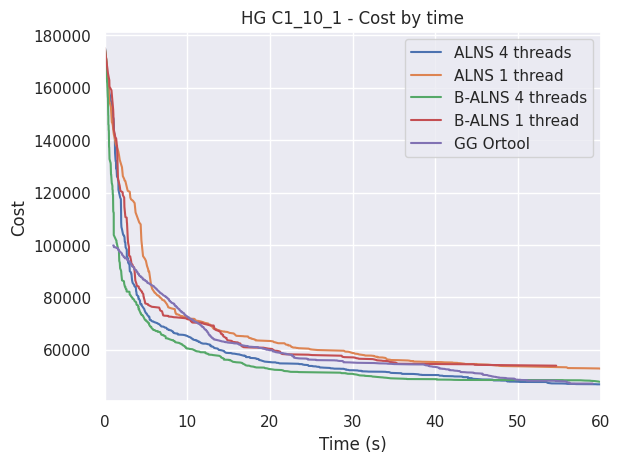
\includegraphics[width=1\linewidth]{figures/cost_time_60s_C1_10_1.png}
    \caption{60s}
    \label{fig:perf_ct_c1_10_60s}
  \end{subfigure}%
  \begin{subfigure}{.5\textwidth}
    \centering
    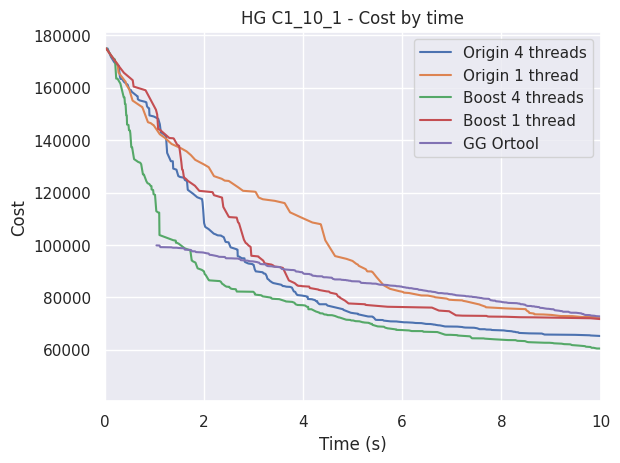
\includegraphics[width=1\linewidth]{figures/cost_time_10s_C1_10_1.png}
    \caption{10s}
    \label{fig:perf_ct_c1_10_10s}
  \end{subfigure}
  \caption{Giá trị hàm mục tiêu theo thời gian, cấu hình C1\_10\_1}
\end{figure}

\begin{figure}[H] % places figure environment here   
  \label{fig:perf_ct_r1_10}
  \begin{subfigure}{.5\textwidth}
    \centering
    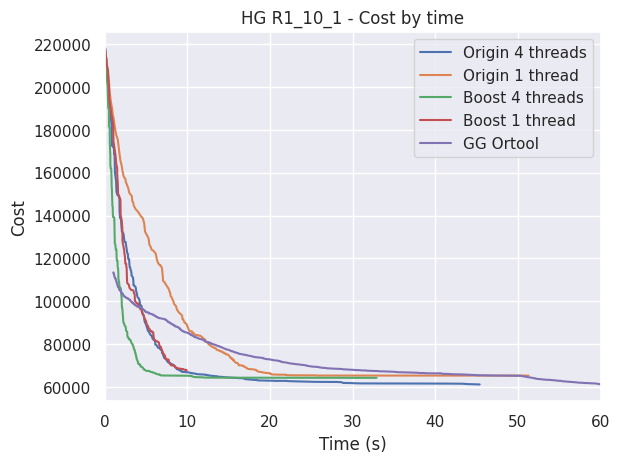
\includegraphics[width=1\linewidth]{figures/cost_time_60s_R1_10_1.png}
    \caption{60s}
    \label{fig:perf_ct_r1_10_60s}
  \end{subfigure}%
  \begin{subfigure}{.5\textwidth}
    \centering
    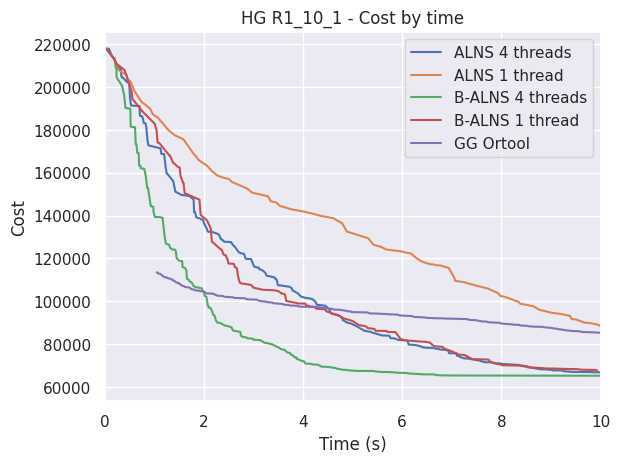
\includegraphics[width=1\linewidth]{figures/cost_time_10s_R1_10_1.png}
    \caption{10s}
    \label{fig:perf_ct_r1_10_10s}
  \end{subfigure}
  \caption{Giá trị hàm mục tiêu theo thời gian, cấu hình R1\_10\_1}
\end{figure}

\begin{figure}[H] % places figure environment here   
  \label{fig:perf_ct_rc1_10}
  \begin{subfigure}{.5\textwidth}
    \centering
    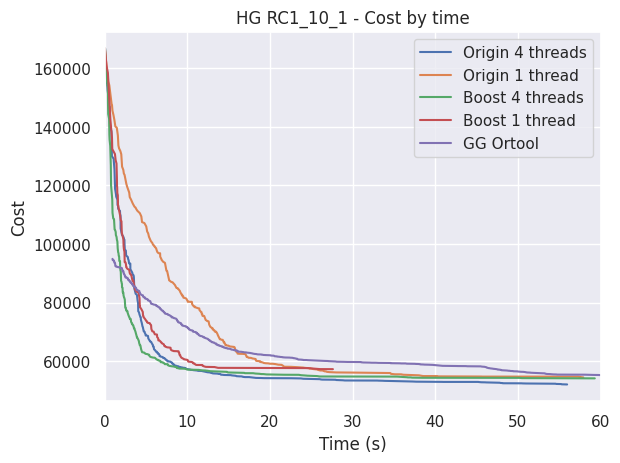
\includegraphics[width=1\linewidth]{figures/cost_time_60s_RC1_10_1.png}
    \caption{60s}
    \label{fig:perf_ct_rc1_10_60s}
  \end{subfigure}%
  \begin{subfigure}{.5\textwidth}
    \centering
    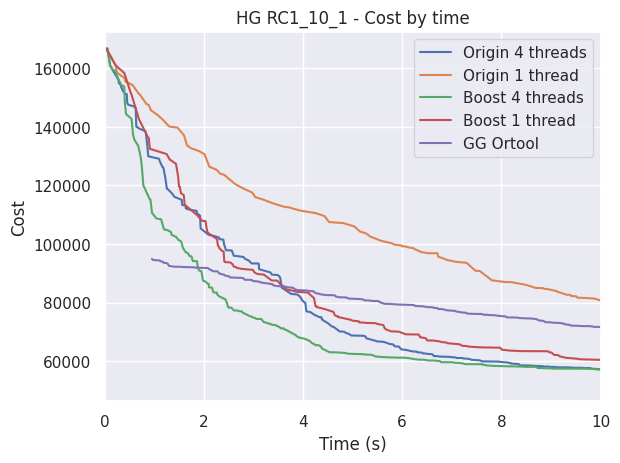
\includegraphics[width=1\linewidth]{figures/cost_time_10s_RC1_10_1.png}
    \caption{10s}
    \label{fig:perf_ct_rc1_10_10s}
  \end{subfigure}
  \caption{Giá trị hàm mục tiêu theo thời gian, cấu hình RC1\_10\_1}
\end{figure}

\begin{figure}[H] % places figure environment here   
  \label{fig:perf_ct_c1_4}
  \begin{subfigure}{.5\textwidth}
    \centering
    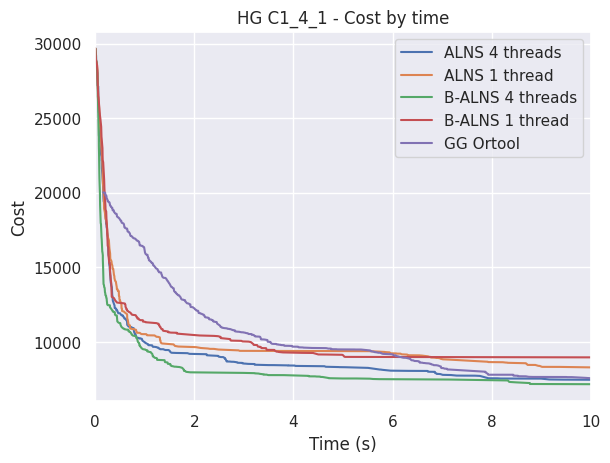
\includegraphics[width=1\linewidth]{figures/cost_time_10s_C1_4_1.png}
    \caption{10s}
    \label{fig:perf_ct_c1_4_10s}
  \end{subfigure}%
  \begin{subfigure}{.5\textwidth}
    \centering
    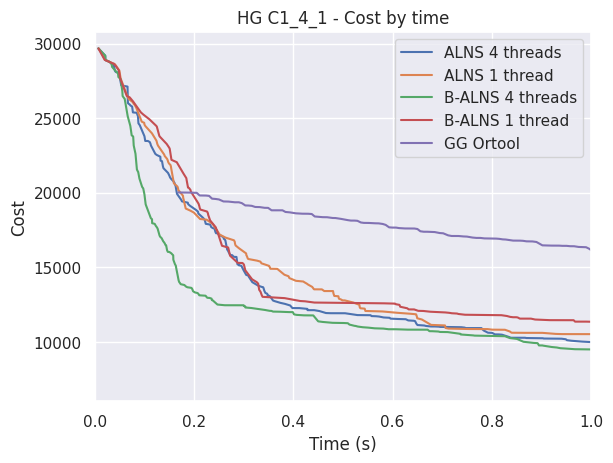
\includegraphics[width=1\linewidth]{figures/cost_time_1s_C1_4_1.png}
    \caption{1s}
    \label{fig:perf_ct_c1_4_1s}
  \end{subfigure}
  \caption{Giá trị hàm mục tiêu theo thời gian, cấu hình C1\_4\_1}
\end{figure}

\begin{figure}[H] % places figure environment here   
  \label{fig:perf_ct_r1}
  \begin{subfigure}{.5\textwidth}
    \centering
    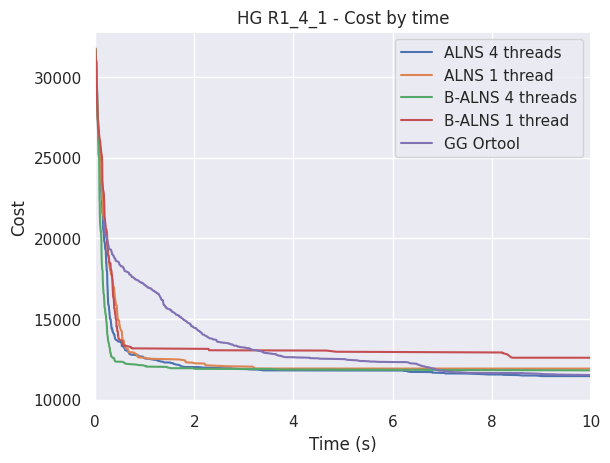
\includegraphics[width=1\linewidth]{figures/cost_time_10s_R1_4_1.png}
    \caption{10s}
    \label{fig:perf_ct_r1_60s}
  \end{subfigure}%
  \begin{subfigure}{.5\textwidth}
    \centering
    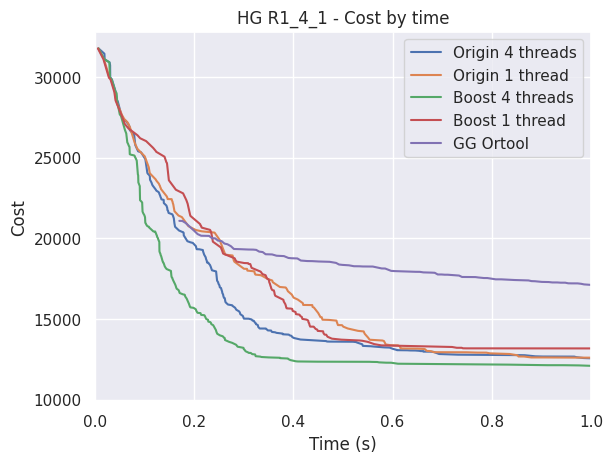
\includegraphics[width=1\linewidth]{figures/cost_time_1s_R1_4_1.png}
    \caption{1s}
    \label{fig:perf_ct_r1_10s}
  \end{subfigure}
  \caption{Giá trị hàm mục tiêu theo thời gian, cấu hình R1\_4\_1}
\end{figure}

\begin{figure}[H] % places figure environment here   
  \label{fig:perf_ct_rc1_4}
  \begin{subfigure}{.5\textwidth}
    \centering
    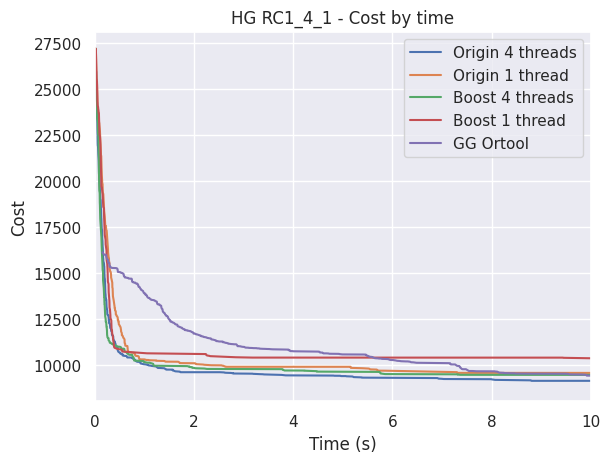
\includegraphics[width=1\linewidth]{figures/cost_time_10s_RC1_4_1.png}
    \caption{10s}
    \label{fig:perf_ct_rc1_4_10s}
  \end{subfigure}%
  \begin{subfigure}{.5\textwidth}
    \centering
    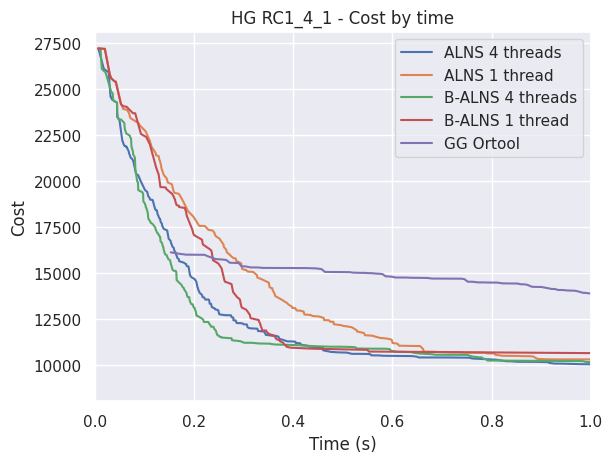
\includegraphics[width=1\linewidth]{figures/cost_time_1s_RC1_4_1.png}
    \caption{1s}
    \label{fig:perf_ct_rc1_4_1s}
  \end{subfigure}
  \caption{Giá trị hàm mục tiêu theo thời gian, cấu hình RC1\_4\_1}
\end{figure}

Với thời gian chạy lâu, các thuật toán đều chững lại bởi khi đó các tuyến đường đã khá chật chội, việc "sửa chữa" là khó khăn hơn giai đoạn đầu rất nhiều. Nói cách khác, thuật toán bị bẫy trong nghiệm tối ưu cục bộ. Khi chạy thuật toán với thời gian lâu hơn (timeout 10 phút), tác giả nhận thấy hàm mục tiêu không giảm đáng kể nữa. Chính vì thế, thời gian chạy 60 giây được lựa chọn để vừa phù hợp với thực tế và tránh việc chạy quá lâu.

Ta thấy một xu hướng rõ ràng, trong giai đoạn đầu, B-ALNS tăng tốc hiệu năng của ALNS một cách đáng kể. Với tập dữ liệu $1000$ yêu cầu, thời gian chạy dưới 10 giây, B-ALNS đơn luồng cho hiệu năng gần như tương đương với ALNS với 4 luồng. Nghĩa là, B-ALNS tiết kiệm khoảng $75\%$ tài nguyên CPU để đạt kết quả tương đương với ALNS trong thời gian chạy dưới 10 giây. Chưa kể, bộ nhớ cũng được tiết kiệm một cách đáng kể khi B-ALNS sử dụng 1 luồng thay vì 4 luồng. Khi so sánh với ALNS đơn luồng, B-ALNS đơn luồng cho hiệu năng vượt trội. Đối với tập dữ liệu có số lượng yêu cầu trung bình ($400$ yêu cầu), B-ALNS đơn luồng không có lợi thế so với ALNS đơn luồng, tuy nhiên hiệu năng đa luồng vẫn tốt hơn ALNS. Điều này cho thấy, B-ALNS có thể được sử dụng để giải quyết các bài toán lớn với tài nguyên hạn chế. Với cấu hình $400$ yêu cầu, B-ALNS đa luồng cho hiệu năng bỏ xa ALNS với thời gian chạy dưới $0.2$ giây và luôn tốt hơn trong thời gian chạy dưới $1$ giây.

Khi so sánh với \code{Google OR-Tools}, ta thấy rằng, \code{Google OR-Tools} cho hiệu năng tốt trong thời gian chạy từ 2 đến 4 giây đầy tiên (tập $1000$ yêu cầu). Tuy nhiên với thời gian chạy dưới 1 giây, \code{Google OR-Tools} không thể cho ra kết quả. Với thời gian chạy lâu hơn, \code{Google OR-Tools} cho hiệu năng không tốt bằng ALNS hay B-ALNS. Với cấu hình $400$ yêu cầu, nhìn chung hiệu năng của B-ALNS cũng như ALNS bỏ xa \code{Google OR-Tools}.

Như vậy đối với các nghiệp vụ yêu cầu một kết quả tốt trong thời gian ngắn, B-ALNS là lựa chọn tốt nhất. Khi tiến hành đo đạc với thời gian chạy dài (timeout lớn hơn 1 phút), tác giả nhận thấy rằng, ALNS là tốt nhất trong các thuật toán được đề cập ở đây. Tuy nhiên chất lượng nghiệm tốt hơn B-ALNS thường không quá $1\%$. Các kết quả được chỉ ra trong phần trước là giá trị hàm mục tiêu khi sử dụng ALNS nguyên bản.

\subsection{Số xe}

Chúng ta cũng nhận thấy một xu hướng tương tự như khi so sánh hiệu năng của các thuật toán khi sử dụng độ đo là giá trị hàm mục tiêu. B-ALNS cho hiệu năng vượt trội trong giai đoạn đầu. B-ALNS đơn luồng cho hiệu năng tương đương với ALNS với 4 luồng. Với cấu hình lớp R ($1000$ yêu cầu), B-ALNS tiết kiệm được khoảng $30\%$ số xe so với ALNS trong thời gian chạy từ 2 tới 4 giây! Tương tự, với cấu hình $400$ yêu cầu, B-ALNS giảm số xe nhanh hơn đáng kể so với ALNS trong thời gian chạy ngắn (dưới $0.2$ giây).  Việc tiết kiệm hàng trăm xe có ý nghĩa rất lớn trong thực tế. Thường thì chi phí cho một xe (thuê, hoặc mua, nhiên liệu, chi phí cho tài xế, ...) là rất lớn. Việc tiết kiệm số xe sẽ giúp giảm chi phí vận hành của doanh nghiệp một cách đáng kể. 

Với thời gian chạy lâu hơn, đương nhiên chúng ta rất khó để giảm được số xe nữa, vì hầu hết các tuyến đường đến lúc này đã chật chội hơn đáng kể so với giai đoạn đầu.

\begin{figure}[H] % places figure environment here   
  \label{fig:perf_ct_c1_10}
  \begin{subfigure}{.5\textwidth}
    \centering
    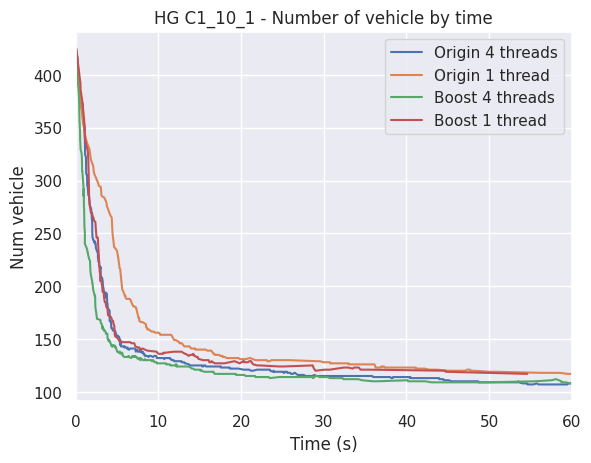
\includegraphics[width=0.9\linewidth]{figures/nv_time_60s_C1_10_1.png}
    \caption{60s}
    \label{fig:perf_ct_c1_10_60s}
  \end{subfigure}%
  \begin{subfigure}{.5\textwidth}
    \centering
    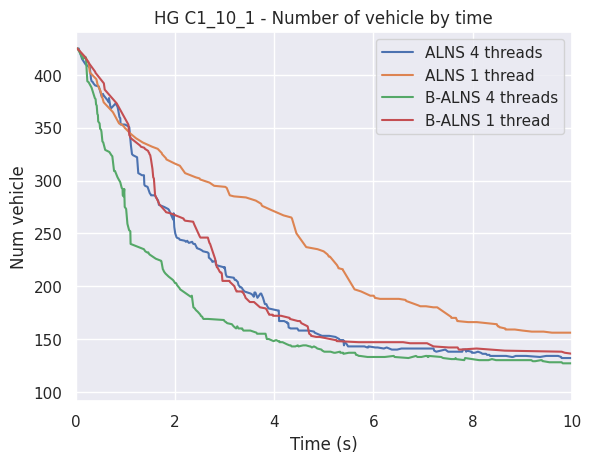
\includegraphics[width=0.9\linewidth]{figures/nv_time_10s_C1_10_1.png}
    \caption{10s}
    \label{fig:perf_ct_c1_10_10s}
  \end{subfigure}
  \caption{Số xe sử dụng theo thời gian, cấu hình C1\_10\_1}
\end{figure}

\begin{figure}[H] % places figure environment here   
  \label{fig:perf_ct_r1_10}
  \begin{subfigure}{.5\textwidth}
    \centering
    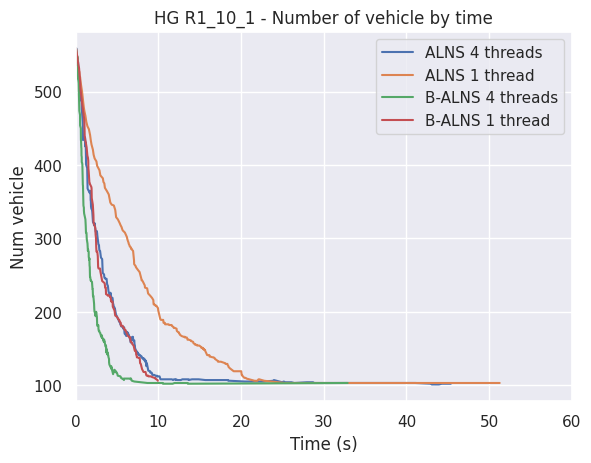
\includegraphics[width=0.9\linewidth]{figures/nv_time_60s_R1_10_1.png}
    \caption{60s}
    \label{fig:perf_ct_r1_10_60s}
  \end{subfigure}%
  \begin{subfigure}{.5\textwidth}
    \centering
    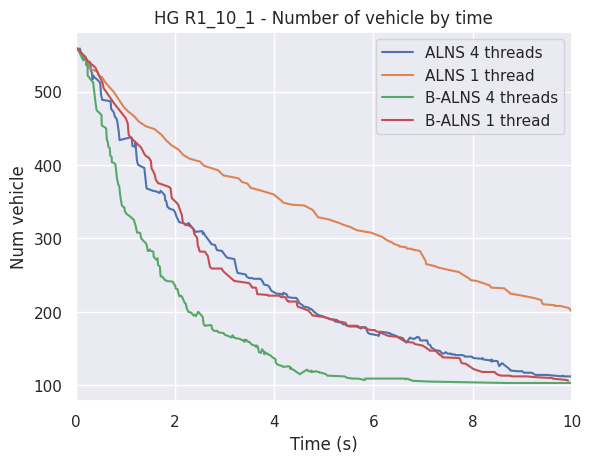
\includegraphics[width=0.9\linewidth]{figures/nv_time_10s_R1_10_1.png}
    \caption{10s}
    \label{fig:perf_ct_r1_10_10s}
  \end{subfigure}
  \caption{Số xe sử dụng theo thời gian, cấu hình R1\_10\_1}
\end{figure}

\begin{figure}[H] % places figure environment here   
  \label{fig:perf_ct_rc1}
  \begin{subfigure}{.5\textwidth}
    \centering
    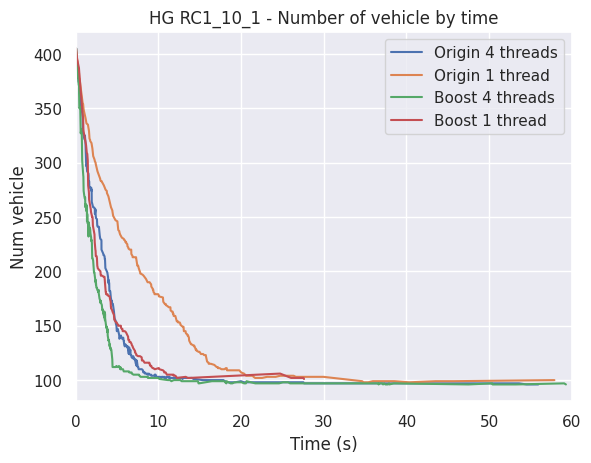
\includegraphics[width=0.9\linewidth]{figures/nv_time_60s_RC1_10_1.png}
    \caption{60s}
    \label{fig:perf_ct_rc1_60s}
  \end{subfigure}%
  \begin{subfigure}{.5\textwidth}
    \centering
    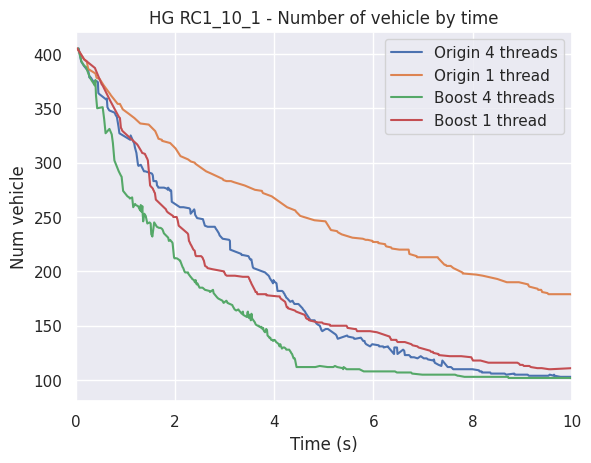
\includegraphics[width=0.9\linewidth]{figures/nv_time_10s_RC1_10_1.png}
    \caption{10s}
    \label{fig:perf_ct_rc1_10s}
  \end{subfigure}
  \caption{Số xe sử dụng theo thời gian, cấu hình RC1\_10\_1}
\end{figure}

\begin{figure}[H] % places figure environment here   
  \label{fig:perf_ct_c1_4}
  \begin{subfigure}{.5\textwidth}
    \centering
    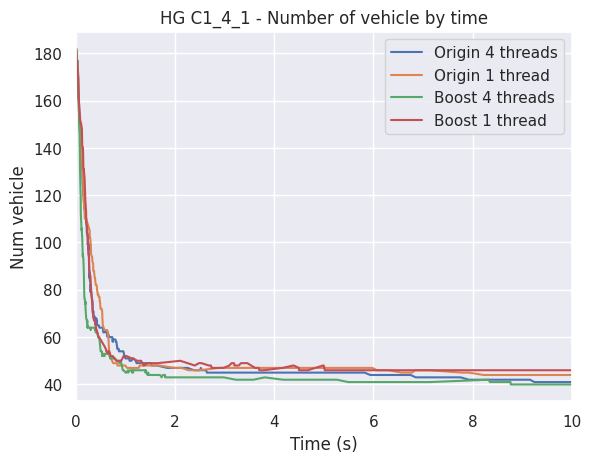
\includegraphics[width=0.9\linewidth]{figures/nv_time_10s_C1_4_1.png}
    \caption{10s}
    \label{fig:perf_ct_c1_4_10s}
  \end{subfigure}%
  \begin{subfigure}{.5\textwidth}
    \centering
    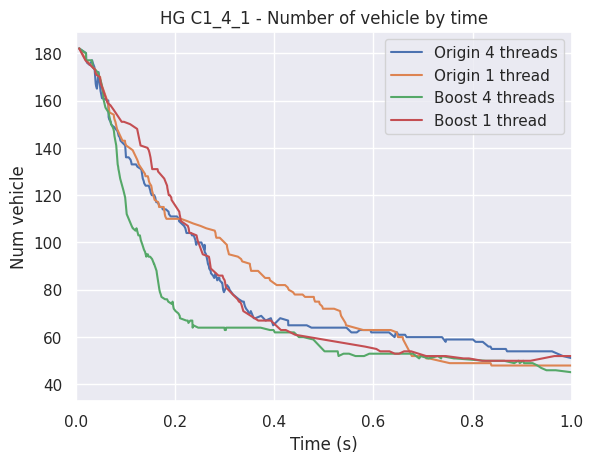
\includegraphics[width=0.9\linewidth]{figures/nv_time_1s_C1_4_1.png}
    \caption{1s}
    \label{fig:perf_ct_c1_4_1s}
  \end{subfigure}
  \caption{Số xe sử dụng theo thời gian, cấu hình C1\_4\_1}
\end{figure}

\begin{figure}[H] % places figure environment here   
  \label{fig:perf_ct_r1_4}
  \begin{subfigure}{.5\textwidth}
    \centering
    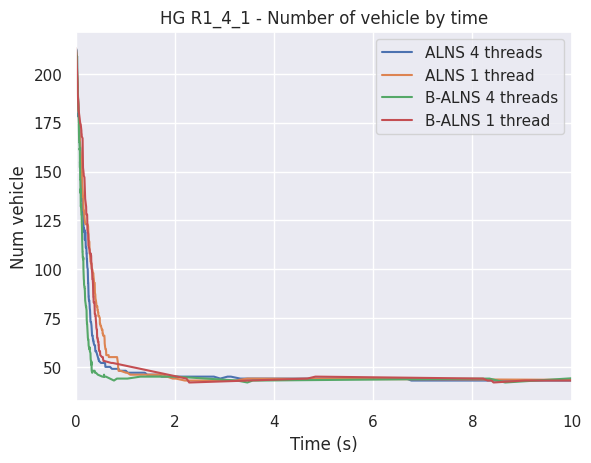
\includegraphics[width=0.9\linewidth]{figures/nv_time_10s_R1_4_1.png}
    \caption{10s}
    \label{fig:perf_ct_r1_4_10s}
  \end{subfigure}%
  \begin{subfigure}{.5\textwidth}
    \centering
    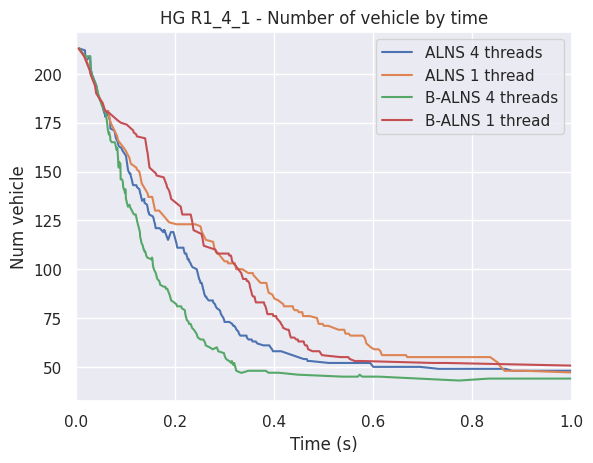
\includegraphics[width=0.9\linewidth]{figures/nv_time_1s_R1_4_1.png}
    \caption{1s}
    \label{fig:perf_ct_r1_4_1s}
  \end{subfigure}
  \caption{Số xe sử dụng theo thời gian, cấu hình R1\_4\_1}
\end{figure}

\begin{figure}[H] % places figure environment here   
  \label{fig:perf_ct_rc1}
  \begin{subfigure}{.5\textwidth}
    \centering
    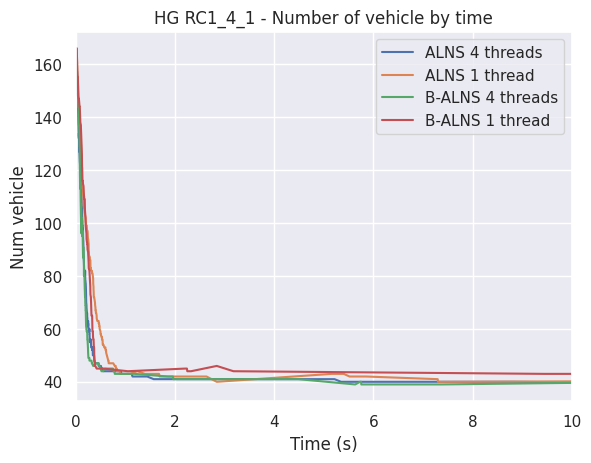
\includegraphics[width=0.9\linewidth]{figures/nv_time_10s_RC1_4_1.png}
    \caption{10s}
    \label{fig:perf_ct_rc1_4_10s}
  \end{subfigure}%
  \begin{subfigure}{.5\textwidth}
    \centering
    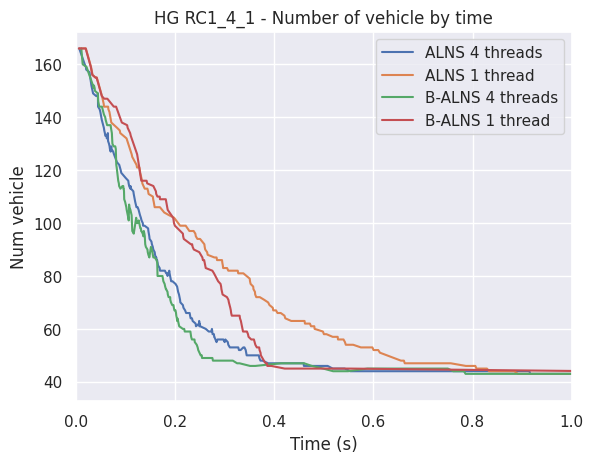
\includegraphics[width=0.9\linewidth]{figures/nv_time_1s_RC1_4_1.png}
    \caption{1s}
    \label{fig:perf_ct_rc1_4_1s}
  \end{subfigure}
  \caption{Số xe sử dụng theo thời gian, cấu hình RC1\_4\_1}
\end{figure}
        \chapter{Kết luận}
\label{chap:conclusion}

Trong luận văn này, tác giả đã nghiên cứu mô hình toán học, các thuật toán giải lớp các bài toán định tuyến xe, đi sâu vào phương pháp tìm kiếm lân cận rộng. Thuật toán \textit{Tìm kiếm lân cận rộng thích ứng - ALNS} được sử dụng để giải bài toán \textit{Định tuyến xe với ràng buộc tải trọng và khung thời gian - VRPTW}. Tác giả đã đề xuất một hiệu chỉnh giúp tăng hiệu năng của ALNS một cách đáng kể được chỉ ra trong kết quả thực nghiệm. Thuật toán được đặt tên là B-ALNS (\textit{Boosted - Adaptive Large Neighborhood Search - Tìm kiếm lân cận rộng thích ứng tăng tốc}). B-ALNS được đánh giá trên các tập dữ liệu thực tế với số lượng yêu cầu (khách hàng) từ trung bình tới rất lớn cho hiệu năng vượt xa ALNS gốc cũng như bộ thư viện phổ biến \code{Google OR-Tools}. Điều này gợi ý sử dụng B-ALNS cho các bài toán thực tế yêu cầu chất lượng nghiệm tốt trong thời gian ngắn. Ngoài ra B-ALNS cũng tiết kiệm tài nguyên tính toán (CPU, bộ nhớ) đáng kể so với ALNS gốc.

Tác giả cũng đã đưa ra gợi ý áp dụng B-ALNS cho tình huống thực tế khi ta cần một phương án định tuyến tốt trong thời gian ngắn. Về lâu dài, nếu mục đích cao nhất là giảm chi phí mà không cần quan tâm tới thời gian chạy, ta nên sử dụng ALNS gốc để đạt được chất lượng nghiệm tốt hơn. Một gợi ý khác là ta có thể sử dụng B-ALNS ở giai đoạn đầu giúp giảm nhanh hàm mục tiêu, sau đó áp dụng ALNS cho giai đoạn sau để tìm nghiệm tốt hơn. Thời điểm chuyển đổi từ B-ALNS sang ALNS có thể là khi hàm mục tiêu giảm không đủ nhiều theo thời gian hay số vòng lặp nữa (theo một ngưỡng nào đó). ALNS cũng như B-ALNS thể hiện tốt về cả chất lượng nghiệm, số xe sử dụng cũng như hiệu năng và độ ổn định khi giải VRPTW với các cấu hình có số lượng yêu cầu không quá lớn (từ $600$ yêu cầu trở xuống). Với các cấu hình mà số lượng yêu cầu là rất lớn (trên $600$ yêu cầu), B-ALNS và ALNS cho chất lượng nghiệm chấp nhận được trong khoảng thời gian chạy ngắn (timeout dưới một phút).

Mở rộng nghiên cứu, tác giả sẽ tiếp tục cải tiến hiệu chỉnh B-ALNS để thu được nghiệm chất lượng hơn cũng như hiệu năng cao hơn nữa. Các tham số khác ngoài số vòng lặp có thể được đưa vào nhiễu hiệu chỉnh trọng số lựa chọn thuật toán. Thời điểm chuyển đổi B-ALNS và ALNS như đã trình bày ở trên cũng sẽ được nghiên cứu tiếp để đưa ra một chiến thuật thích ứng hợp lý để thuật toán vừa chạy nhanh mà vẫn thu được nghiệm tốt. Thêm vào đó, tác giả tiếp tục nghiên cứu cơ chế thích ứng để "bỏ đi" và "thêm lại" yêu cầu với số lượng hợp lý theo trạng thái của hệ nhằm cải thiện chất lượng nghiệm cũng như tăng hiệu năng.


    \end{content}
    
    \pagenumbering{Roman}
    \setcounter{page}{\numexpr\value{savepage}}

    % References
    \references{}

    
    % Appendix
    %  \begin{appendix}
    %     % In the appendices, use \section{} instead of \chapter{}
    %      \section{Some Appendix Section}
\label{sec:appendix01}
Appendices provide only two structural levels, viz., \texttt{\textbackslash section}, and \texttt{\textbackslash subsection}.

The numbering of figures, listings, tables, and footnotes is not reset. Thus, it continues as usual in the appendix.

\subsection{Some Appendix Subsection}

\lipsum[10]
    %  \end{appendix}




    % Declaration of authorship
    % \authorshipstatement[pagenumbering=false]
    % \authorshipstatement[pagenumbering=true]
    % \authorshipstatement[pagenumbering=only]
    
    % Consent form for use of plagiarism detection software
    % Not yet required
    % \consentform[pagenumbering=false]
    % \consentform[pagenumbering=true]
    % \consentform[pagenumbering=only]
    
    % Bonus: Wordcount
    % cd %FOLDER WHERE THE .tex FILES ARE IN %
    % clear
    % texcount -total -q -col -sum *.tex
    
\end{document}
